%!!!!!!!! add patient numbers?
%% since this is going in before the paper pub, we need to say that 
% we are going to do the arps as well.
% aim1: how does MCHAT correlate with arps risk. Does this relationship vary with other parameters . Are there confounders that we can eliminate. We can do continuous evaluation which cannot be done for MCHAT (absense of recoirds oia slso informative)

% aim2: Head to head comparison Mchat, other protocols vs ars. Is there reduction in waittimes and falsle positives. Is there boost in sensitivy?

% aim2a: combined operation: feasibility and efficacy design issues, dependence on location of facility. Is this universal. To what degree do we need to retrain as we move from clinic to next?

% aim3: demographic dependence, diverse population. How much impact is there using arps?


% aim4: chracrerization of heterogeneity


%interaction with screening tools (Primarily M-CHAT)
%minorities and sub-populations
%separate ASD from other conditions (cerebral palsy, non-ASD developmental delay) - with different causal pathways

%combined performance -> when you trigger what actually happens
%test combined performance


%when we talk about the intended benefits, we need to be clear on whether reduced wait time is fewer false positives clogging the system vs earlier identification (or both). Just need to be clear that it wont be because our team administering ADOS sees people
%faster..


%Those mentioned were
%Gastroinstestinal (esp. Constirpation)
%Allergies
%Prematurity (basically 765.X ICD9s)
%Infections (different categories of them)
%Abrupt development worsening (after ~ 12 to 18 months)

\documentclass[onecolumn, compsoc,11pt]{IEEEtran}
\usepackage{enumitem}
\usepackage{etex}
\usepackage{amssymb,amsfonts,amsmath,amsthm}
\usepackage{graphicx}
\usepackage[usenames,x11names, dvipsnames, svgnames]{xcolor}
\usepackage{amsmath,amssymb}
\usepackage{dsfont}
\usepackage{amsfonts}
\usepackage{mathrsfs}
\usepackage{texshade}
\usepackage{multirow}
\usepackage{hyperref}
\hypersetup{
  colorlinks=true,
  linkcolor=black,
  citecolor=black,
  filecolor=black,
  urlcolor=DodgerBlue4,
  breaklinks=false,
  % linkbordercolor=red,% hyperlink borders will be red
  % pdfborderstyle={/S/U/W 1}% border style will be underline of width 1pt
}
\usepackage{array}
\usepackage{xr}
\usepackage{verbatim}
% \usepackage{multirow}    
% \usepackage[T1,euler-digits]{eulervm}
% \usepackage{times}
% \usepackage{pxfonts}
\usepackage{tikz}
\usepackage{pgfplots}
\usetikzlibrary{shapes,calc,shadows,fadings,arrows,decorations.pathreplacing,automata,positioning}
\usetikzlibrary{external}
\usetikzlibrary{decorations.text}
\usepgfplotslibrary{colorbrewer} 

\tikzexternalize[prefix=./Figures/External/]% activate externalization!
\tikzexternaldisable
% \addtolength{\voffset}{.1in}  
\usepackage{geometry}
\geometry{a4paper, left=.65in,right=.65in,top=.8in,bottom=0.7in}

\addtolength{\textwidth}{-.1in}    
\addtolength{\hoffset}{.05in}    
\addtolength{\textheight}{0in}    
\addtolength{\footskip}{0in}    
\usepackage{rotating}
\definecolor{nodecol}{RGB}{240,240,220}
\definecolor{nodeedge}{RGB}{240,240,225}
\definecolor{edgecol}{RGB}{130,130,130}
\tikzset{%
  fshadow/.style={      preaction={
      fill=black,opacity=.3,
      path fading=circle with fuzzy edge 20 percent,
      transform canvas={xshift=1mm,yshift=-1mm}
    }} 
}
\usetikzlibrary{pgfplots.dateplot}
\usetikzlibrary{patterns}
\usetikzlibrary{decorations.markings}
\usepackage{fancyhdr}
\usepackage{mathtools}
\usepackage{datetime}
\usepackage{comment}
%% ## Equation Space Control---------------------------
\def\EQSP{3pt}
\newcommand{\mltlne}[2][\EQSP]{\begingroup\setlength\abovedisplayskip{#1}\setlength\belowdisplayskip{#1}\begin{equation}\begin{multlined} #2 \end{multlined}\end{equation}\endgroup\noindent}
\newcommand{\cgather}[2][\EQSP]{\begingroup\setlength\abovedisplayskip{#1}\setlength\belowdisplayskip{#1}\begin{gather} #2 \end{gather}\endgroup\noindent}
\newcommand{\cgathers}[2][\EQSP]{\begingroup\setlength\abovedisplayskip{#1}\setlength\belowdisplayskip{#1}\begin{gather*} #2 \end{gather*}\endgroup\noindent}
\newcommand{\calign}[2][\EQSP]{\begingroup\setlength\abovedisplayskip{#1}\setlength\belowdisplayskip{#1}\begin{align} #2 \end{align}\endgroup\noindent}
\newcommand{\caligns}[2][\EQSP]{\begingroup\setlength\abovedisplayskip{#1}\setlength\belowdisplayskip{#1}\begin{align*} #2 \end{align*}\endgroup\noindent}
\newcommand{\mnp}[2]{\begin{minipage}{#1}#2\end{minipage}} 
%% COLOR DEFS------------------------------------------
\newtheorem{thm}{Theorem}
\newtheorem{cor}{Corollary}
\newtheorem{lem}{Lemma}
\newtheorem{prop}{Proposition}
\newtheorem{defn}{Definition}
\newtheorem{exmpl}{Example}
\newtheorem{rem}{Remark}
\newtheorem{notn}{Notation}
%% ------------PROOF INCLUSION -----------------
\def\NOPROOF{Proof omitted.}
\newif\ifproof
\prooffalse % or \draftfalse
\newcommand{\Proof}[1]{
  \ifproof
  \begin{IEEEproof}
    #1\end{IEEEproof}
  \else
  \NOPROOF
  \fi
}
%% ------------ -----------------
\newcommand{\DETAILS}[1]{#1}
%% ------------ -----------------
% color commands------------------------
\newcommand{\etal}{\textit{et} \mspace{3mu} \textit{al.}}
% \renewcommand{\algorithmiccomment}[1]{$/** $ #1 $ **/$}
\newcommand{\vect}[1]{\textbf{\textit{#1}}}
\newcommand{\figfont}{\fontsize{8}{8}\selectfont\strut}
\newcommand{\hlt}{ \bf \sffamily \itshape\color[rgb]{.1,.2,.45}}
\newcommand{\pitilde}{\widetilde{\pi}}
\newcommand{\Pitilde}{\widetilde{\Pi}}
\newcommand{\bvec}{\vartheta}
\newcommand{\algo}{\textrm{\bf\texttt{GenESeSS}}\xspace}
\newcommand{\xalgo}{\textrm{\bf\texttt{xGenESeSS}}\xspace}
\newcommand{\FNTST}{\bf }
\newcommand{\FNTED}{\color{darkgray} \scriptsize $\phantom{.}$}
\renewcommand{\baselinestretch}{.95}
\newcommand{\sync}{\otimes}
\newcommand{\psync}{\hspace{3pt}\overrightarrow{\hspace{-3pt}\sync}}
% \newcommand{\psync}{\raisebox{-4pt}{\begin{tikzpicture}\node[anchor=south] (A) {$\sync$};
%   \draw [->,>=stealth] ([yshift=-2pt, xshift=2pt]A.north west) -- ([yshift=-2pt]A.north east); %\end{tikzpicture}}}
\newcommand{\base}[1]{\llbracket #1 \rrbracket}
\newcommand{\nst}{\textrm{\sffamily\textsc{Numstates}}}
\newcommand{\HA}{\boldsymbol{\mathds{H}}}
\newcommand{\eqp}{ \vartheta }
\newcommand{\entropy}[1]{\boldsymbol{h}\left ( #1 \right )}
\newcommand{\norm}[1]{\left\lVert #1 \right\rVert}%
\newcommand{\abs}[1]{\left\lvert #1 \right\rvert}%
\newcommand{\absB}[1]{\big\lvert #1 \big\rvert}%
% #############################################################
% #############################################################
% PREAMBLE ####################################################
% #############################################################
% #############################################################
% \usepackage{pnastwoF}      
\DeclareMathOperator*{\argmax}{argmax}
\DeclareMathOperator*{\argmin}{arg\,min}
\DeclareMathOperator*{\expect}{\mathbf{E}}
\DeclareMathOperator*{\var}{\mathbf{Var}}

\newcommand{\ND}{ \mathcal{N}  }
\usepackage[linesnumbered,ruled,vlined,noend]{algorithm2e}
\newcommand{\captionN}[1]{\caption{\color{darkgray} \sffamily \fontsize{9}{11}\selectfont #1  }}
\newcommand{\btl}{\ \textbf{\small\sffamily bits/letter}}
\usepackage{txfonts}
% \usepackage{ccfonts}
%%% save defaults
\renewcommand{\rmdefault}{phv} % Arial
\renewcommand{\sfdefault}{phv} % Arial
\edef\keptrmdefault{\rmdefault}
\edef\keptsfdefault{\sfdefault}
\edef\keptttdefault{\ttdefault}

% \usepackage{kerkis}
\usepackage[OT1]{fontenc}
\usepackage{concmath}
% \usepackage[T1]{eulervm} 
% \usepackage[OT1]{fontenc}
%%% restore defaults
\edef\rmdefault{\keptrmdefault}
\edef\sfdefault{\keptsfdefault}
\edef\ttdefault{\keptttdefault}
\tikzexternalenable
% ##########################################################
\tikzfading[name=fade out,
inner color=transparent!0,
outer color=transparent!100]
% ###################################
\newcommand{\xtitaut}[2]{
  \noindent\mnp{\textwidth}{
    \mnp{\textwidth}{\raggedright\Huge \bf \sffamily #1}

    \vskip 1em

    {\bf \sffamily #2}
  }
  \vskip 2em
}
% ###################################
% ###################################
\tikzset{wiggle/.style={decorate, decoration={random steps, amplitude=10pt}}}
\usetikzlibrary{decorations.pathmorphing}
\pgfdeclaredecoration{Snake}{initial}
{
  \state{initial}[switch if less than=+.625\pgfdecorationsegmentlength to final,
  width=+.3125\pgfdecorationsegmentlength,
  next state=down]{
    \pgfpathmoveto{\pgfqpoint{0pt}{\pgfdecorationsegmentamplitude}}
  }
  \state{down}[switch if less than=+.8125\pgfdecorationsegmentlength to end down,
  width=+.5\pgfdecorationsegmentlength,
  next state=up]{
    \pgfpathcosine{\pgfqpoint{.25\pgfdecorationsegmentlength}{-1\pgfdecorationsegmentamplitude}}
    \pgfpathsine{\pgfqpoint{.25\pgfdecorationsegmentlength}{-1\pgfdecorationsegmentamplitude}}
  }
  \state{up}[switch if less than=+.8125\pgfdecorationsegmentlength to end up,
  width=+.5\pgfdecorationsegmentlength,
  next state=down]{
    \pgfpathcosine{\pgfqpoint{.25\pgfdecorationsegmentlength}{\pgfdecorationsegmentamplitude}}
    \pgfpathsine{\pgfqpoint{.25\pgfdecorationsegmentlength}{\pgfdecorationsegmentamplitude}}
  }
  \state{end down}[width=+.3125\pgfdecorationsegmentlength,
  next state=final]{
    \pgfpathcosine{\pgfqpoint{.15625\pgfdecorationsegmentlength}{-.5\pgfdecorationsegmentamplitude}}
    \pgfpathsine{\pgfqpoint{.15625\pgfdecorationsegmentlength}{-.5\pgfdecorationsegmentamplitude}}
  }
  \state{end up}[width=+.3125\pgfdecorationsegmentlength,
  next state=final]{
    \pgfpathcosine{\pgfqpoint{.15625\pgfdecorationsegmentlength}{.5\pgfdecorationsegmentamplitude}}
    \pgfpathsine{\pgfqpoint{.15625\pgfdecorationsegmentlength}{.5\pgfdecorationsegmentamplitude}}
  }
  \state{final}{\pgfpathlineto{\pgfpointdecoratedpathlast}}
}
% ###################################
% ###################################
\newcolumntype{L}[1]{>{\rule{0pt}{2ex}\raggedright\let\newline\\\arraybackslash\hspace{0pt}}m{#1}}
\newcolumntype{C}[1]{>{\rule{0pt}{2ex}\centering\let\newline\\\arraybackslash\hspace{0pt}}m{#1}}
\newcolumntype{R}[1]{>{\rule{0pt}{2ex}\raggedleft\let\newline\\\arraybackslash\hspace{0pt}}m{#1}}




\newcommand{\drhh}[8]{
  \begin{axis}[semithick,
    font=\bf \sffamily \fontsize{7}{7}\selectfont,
    name=H2,
    at=(#4), anchor=#5,
    xshift=.3in,
    yshift=-.3in,
    width=\WDT, 
    height=\HGT, 
    title={{\LARGE G } ROC area distribution (Out-of-sample)}, 
    title style={align=right, },legend cell align=left,
    legend style={ xshift=3.5in, yshift=-.6in, draw=white, fill= gray, fill opacity=0.2, 
      text opacity=1,},
    axis line style={black!80, opacity=0,   thick,,ultra thin, rounded corners=0pt},
    axis on top=false, 
    xlabel={ROC area},
    ylabel={probability},
    ylabel style={yshift=-.25in},
    xlabel style={yshift=.1in},
    grid style={dashed, gray!50},
    % grid,
    axis background/.style={top color=gray!1,bottom color=gray!2},
    enlargelimits=false, 
    scale only axis=true,
    ymin=0,
    % xmin=.7,xmax=1.0,
    ylabel style={yshift=.05in},
    major tick length=0pt,yticklabel style={/pgf/number format/fixed,/pgf/number format/precision=2},xticklabel style={/pgf/number format/fixed,/pgf/number format/precision=2},
    #7,
    ]
    \addplot [
    fill=#8,
    thick,
    draw=white,
    opacity=1,
    hist={density,bins=10},
    ] table [y index=#3] {#1};
    % \addlegendentry{$\Delta$ ROC};
    \addplot [very thick, Red2,, opacity=.95] gnuplot [raw gnuplot] {plot '#1' u #2:(1./#6.) smooth kdensity};
    % 
    % \draw[thin,black ] (axis cs:.89291,\pgfkeysvalueof{/pgfplots/ymin}) -- (axis cs:.89291,\pgfkeysvalueof{/pgfplots/ymax}) node [midway,right, pos=0.2] {89.3\%};
    % \addlegendentry{kde};
  \end{axis}
}


\newcommand{\erhh}[6]{
  \begin{axis}[semithick,
    font=\bf \sffamily \fontsize{7}{7}\selectfont,
    name=H2,
    at=(#3), anchor=#4,
    xshift=.3in,
    yshift=-.3in,
    width=\WDT, 
    height=\HGT, 
    title style={align=center, },legend cell align=left,
    legend style={ xshift=3.5in, yshift=-.6in, draw=white, fill= gray, fill opacity=0.2, 
      text opacity=1,},
    axis line style={black!80, opacity=0,   thick,,ultra thin, rounded corners=0pt},
    axis on top=false, 
    xlabel={ROC area},
    ylabel={probability},
    ylabel style={yshift=-.25in},
    xlabel style={yshift=.1in},
    grid style={dashed, gray!50},
    % grid,
    axis background/.style={top color=gray!1,bottom color=gray!2},
    enlargelimits=false, 
    scale only axis=true,
    % ymin=0, 
    % xmin=.7,xmax=1.0,
    ylabel style={yshift=.05in},
    major tick length=0pt,yticklabel style={/pgf/number format/fixed,/pgf/number format/precision=2},xticklabel style={/pgf/number format/fixed,/pgf/number format/precision=2},
    #5,
    ]
    \addplot[semithick, #6]
    table[x expr=(\coordindex+1),y expr=(\thisrowno{#2})] {#1};
    % \addlegendentry{Cullman, Alabama};
  \end{axis}
}
% ################################################
% ################################################
% ################################################
% ################################################
\def\DISCLOSURE#1{\def\disclosure{#1}}
\DISCLOSURE{\raisebox{15pt}{$\phantom{XxxX}$This sheet contains proprietary information 
    not to be released to third parties except for the explicit purpose of evaluation.}
}
% ####################################
\newcommand{\set}[1]{\left\{ #1 \right\}}
\newcommand{\paren}[1]{\left( #1 \right)}
\newcommand{\bracket}[1]{\left[ #1 \right]}
% \newcommand{\norm}[1]{\left\Vert #1 \right\Vert}
\newcommand{\nrm}[1]{\left\llbracket{#1}\right\rrbracket}
\newcommand{\parenBar}[2]{\paren{#1\,{\left\Vert\,#2\right.}}}
\newcommand{\parenBarl}[2]{\paren{\left.#1\,\right\Vert\,#2}}
\newcommand{\ie}{$i.e.$\xspace}
\newcommand{\addcitation}{\textcolor{black!50!red}{\textbf{ADD CITATION}}}
\newcommand{\subtochange}[1]{{\color{black!50!green}{#1}}}
\newcommand{\tobecompleted}{{\color{black!50!red}TO BE COMPLETED.}}


\newcommand{\pIn}{\mathscr{P}_{\textrm{in}}}
\newcommand{\pOut}{\mathscr{P}_{\textrm{out}}}
\newcommand{\aIn}[1][\Sigma]{#1_{\textrm{in}}}
\newcommand{\aOut}[1][\Sigma]{#1_{\textrm{out}}}
\newcommand{\xin}[1]{#1_{\textrm{in}}}
\newcommand{\xout}[1]{#1_{\textrm{out}}}

\newcommand{\R}{\mathbb{R}} % Set of real numbers
\newcommand{\F}[1][]{\mathcal{F}_{#1}}
\newcommand{\SR}{\mathcal{S}} % Semiring of sets
\newcommand{\RR}{\mathcal{R}} % Ring of sets
\newcommand{\N}{\mathbb{N}} % Set of natural numbers (0 included)


\newcommand{\Pp}[1][n]{\mathscr{P}^+_{#1}}
\renewcommand{\entropy}[1]{\boldsymbol{h}\left ( #1 \right )}



\makeatletter
\pgfdeclarepatternformonly[\hatchdistance,\hatchthickness]{flexible hatch}
{\pgfqpoint{0pt}{0pt}}
{\pgfqpoint{\hatchdistance}{\hatchdistance}}
{\pgfpoint{\hatchdistance-1pt}{\hatchdistance-1pt}}%
{
  \pgfsetcolor{\tikz@pattern@color}
  \pgfsetlinewidth{\hatchthickness}
  \pgfpathmoveto{\pgfqpoint{0pt}{0pt}}
  \pgfpathlineto{\pgfqpoint{\hatchdistance}{\hatchdistance}}
  \pgfusepath{stroke}
}
\makeatother

\pgfdeclarepatternformonly{north east lines wide}%
{\pgfqpoint{-1pt}{-1pt}}%
{\pgfqpoint{10pt}{10pt}}%
{\pgfqpoint{9pt}{9pt}}%
{
  \pgfsetlinewidth{0.7pt}
  \pgfpathmoveto{\pgfqpoint{0pt}{0pt}}
  \pgfpathlineto{\pgfqpoint{9.1pt}{9.1pt}}
  \pgfusepath{stroke}
}

\pgfdeclarepatternformonly{north west lines wide}%
{\pgfqpoint{-1pt}{-1pt}}%
{\pgfqpoint{10pt}{10pt}}%
{\pgfqpoint{9pt}{9pt}}%
{
  \pgfsetlinewidth{0.7pt}
  \pgfpathmoveto{\pgfqpoint{0pt}{9pt}}
  \pgfpathlineto{\pgfqpoint{9.1pt}{-0.1pt}}
  \pgfusepath{stroke}
}
\makeatletter

\pgfdeclarepatternformonly[\hatchdistance,\hatchthickness]{flexible hatchB}
{\pgfqpoint{0pt}{\hatchdistance}}
{\pgfqpoint{\hatchdistance}{0pt}}
{\pgfpoint{1pt}{\hatchdistance-1pt}}%
{
  \pgfsetcolor{\tikz@pattern@color}
  \pgfsetlinewidth{\hatchthickness}
  \pgfpathmoveto{\pgfqpoint{0pt}{\hatchdistance}}
  \pgfpathlineto{\pgfqpoint{\hatchdistance}{0pt}}
  \pgfusepath{stroke}
}    \makeatother


\def\TPR{\textrm{TPR}\xspace}
\def\TNR{\textrm{TNR}\xspace}
\def\FPR{\textrm{FPR}\xspace}
\def\PPV{\textrm{PPV}\xspace}

\usetikzlibrary{arrows.meta}
\usetikzlibrary{decorations.pathreplacing,shapes.misc}
\usepgfplotslibrary{fillbetween}
%\usepackage{tikz-network}
\usetikzlibrary{shapes.geometric}
\usetikzlibrary{math}
\usepgfplotslibrary{colorbrewer} 

\usepackage{textcomp}
\usepackage{colortbl}
\usepackage{array}
\usepackage{courier} 
\usepackage{wrapfig}
\usepackage{pifont}
\usetikzlibrary{chains,backgrounds}
\usetikzlibrary{intersections}
\usetikzlibrary{pgfplots.groupplots}
\usepgfplotslibrary{fillbetween} 
\usetikzlibrary{arrows.meta}
\usepackage{pgfplotstable}
%\usepackage[super,compress,sort,comma]{natbib}
\usepackage{setspace}
\usetikzlibrary{math}
\usetikzlibrary{matrix}
\usepackage{xstring}
\usepackage{xspace}
\usepackage{flushend}
\makeatletter
\renewcommand\section{\@startsection {section}{1}{\z@}%
  {-2ex \@plus -1ex \@minus -.2ex}%
  {1ex \@plus.1ex}%
  {\Large\bfseries\scshape}}
\renewcommand\subsection{\@startsection {section}{1}{\z@}%
  {-2ex \@plus -.25ex \@minus -.2ex}%
  {0.1ex \@plus.0ex}%
  {\fontsize{11}{10}\selectfont\bfseries\sffamily\color{black}}}
\renewcommand\subsubsection{\@startsection {section}{1}{\z@}%
  {0ex \@plus -.5ex \@minus -.2ex}%
  {0.0ex \@plus.5ex}%
  {\fontsize{9}{9}\selectfont\bfseries\itshape\sffamily\color{darkgray}}}
\renewcommand\paragraph{\@startsection {section}{1}{\z@}%
  {-.2ex \@plus -.5ex \@minus -.2ex}%
  {0.0ex \@plus.5ex}%
  {\fontsize{9}{9}\selectfont\itshape\sffamily\color{darkgray}}}
   
 
\makeatother
\makeatletter
\pgfdeclareradialshading[tikz@ball]{ball}{\pgfqpoint{-10bp}{10bp}}{%
  color(0bp)=(tikz@ball!30!white);
  color(9bp)=(tikz@ball!75!white);
  color(18bp)=(tikz@ball!90!black);
  color(25bp)=(tikz@ball!70!black);
  color(50bp)=(black)}
\makeatother
\newcommand{\tball}[1][CadetBlue4]{${\color{#1}\Large\boldsymbol{\blacksquare}}$}
\renewcommand{\baselinestretch}{1}
\renewcommand{\captionN}[1]{\caption{\color{CadetBlue4!50!black} \sffamily \fontsize{9}{10}\selectfont #1  }}
\tikzexternaldisable 
\parskip=6pt
\parindent=0pt
\newcommand{\Mark}[1]{\textsuperscript{#1}}
\pagestyle{fancy}

\newcounter{Dcounter}
\setcounter{Dcounter}{1}
\newcommand{\DQS}[1]{\ifdraftQ
{\marginpar{\tikzexternaldisable \tikz{\node[rounded corners=5pt,draw=none,thick,fill=black!10,font=\sffamily\fontsize{7}{8}\selectfont] {\mnp{.45in} {\color{Red3}\raggedright  \#\theDcounter.~#1}}; }}}\stepcounter{Dcounter}\xspace
\fi}

\newcommand{\qn}[1][i]{\Phi_{#1}}
\newcommand{\D}[1][i]{\mathscr{D}\left ( {\Sigma_#1} \right ) }
\newcommand{\Dx}{\mathscr{D}}
\def\J{\mathds{J}}
\def\M{\omega}
\def\N{\mathds{N}}
\newcommand{\cp}[1][P]{\langle #1 \rangle}
\newcommand{\mem}[1]{\M_{#1}}  
\usepackage{textcomp}
\usepackage{colortbl}
\usepackage{subfigure}
\usepackage{array}
\usepackage{courier}
\usepackage{setspace}
\usepackage{wrapfig}
\usepackage{calligra}
\usepackage{ulem}
\usepackage{multirow}

\usetikzlibrary{chains,backgrounds}
\usetikzlibrary{intersections}
\usepackage[super]{cite} 
\makeatletter \renewcommand{\@citess}[1]{\raisebox{1pt}{\textsuperscript{[#1]}}} \makeatother
\usepackage{xstring}
\usepackage{wasysym}
\usepackage[misc]{ifsym}
\renewcommand{\thesectiondis}{\arabic{section}.}
\renewcommand{\thesubsectiondis}{\arabic{section}.\arabic{subsection}.}

\makeatletter
\renewcommand\section{\@startsection {section}{1}{\z@}%
                                   {-1pt \@plus -30ex \@minus 20ex}%
                                   {.1pt}%
                                   {\large\bfseries\scshape}}
\renewcommand\subsection{\@startsection {subsection}{2}{\z@}%
                                   {0ex \@plus -1.75ex \@minus -1.2ex}%
                                   {0ex \@plus.0ex}%
                                   {\fontsize{11}{11}\selectfont\bfseries\sffamily\color{black}}}
\renewcommand\subsubsection{\@startsection {section}{1}{\z@}%
                                   {-1.5ex \@plus -.5ex \@minus -.2ex}%
                                   {0.0ex \@plus.5ex}%
                                   {\fontsize{9}{9}\selectfont\bfseries\sffamily\color{Red4}}}
\renewcommand\paragraph{\@startsection {section}{1}{\z@}%
                                   {-.1ex \@plus -.5ex \@minus -.2ex}%
                                   {0.0ex \@plus.5ex}%
                                   {\fontsize{11}{10}\selectfont\bfseries\itshape\sffamily\color{black}}}
\makeatother
 
                          
\makeatletter
\pgfdeclareradialshading[tikz@ball]{ball}{\pgfqpoint{-10bp}{10bp}}{%
 color(0bp)=(tikz@ball!30!white);
 color(9bp)=(tikz@ball!75!white);
 color(18bp)=(tikz@ball!90!black);
 color(25bp)=(tikz@ball!70!black);
 color(50bp)=(black)}
\makeatother
\newcommand{\tball}{${\color{CadetBlue3}\Large\boldsymbol{\blacksquare}}$}
\renewcommand{\baselinestretch}{.95}
\newcommand{\VSP}{\vspace{-2pt}}
\renewcommand{\captionN}[1]{\caption{\color{CadetBlue4!80!black} \sffamily \fontsize{9}{10}\selectfont #1  }}
\tikzexternaldisable 
\parskip=6pt
\parindent=0pt
\newcommand{\Mark}[1]{\textsuperscript{#1}}
\lhead{}
\pagestyle{fancy}
\def\COLA{black}
%###################################
\cfoot{\bf\sffamily \scriptsize \color{Maroon!50} I. Chattopadhyay, Department of Medicine, University of Chicago}
\cfoot{}
\rhead{}
%\rhead{\bf\sffamily \scriptsize \color{DodgerBlue4!50} DARPA Young Faculty Award 2017}
%\rhead{\scriptsize\bf\sffamily \href{zed.UChicago.edu}{zed.UChicago.edu}}
%\rfoot{\scriptsize\bf\sffamily\thepage}
\newcommand{\partxt}{\bf\sffamily\itshape}
%############################################################
\newif\iftikzX
\tikzXtrue
\tikzXfalse

\newcommand\guline{\bgroup\markoverwith
{\textcolor{black!30}{\rule[-0.45ex]{2pt}{0.4pt}}}\ULon}
\newcommand\hilit[1]{\textcolor{Red1}{#1}}
\newcommand\hilitx[1]{\guline{#1}}
%############################################################
\addtolength{\voffset}{.1in}
\addtolength{\textwidth}{-.085in}
\addtolength{\hoffset}{.0425in}
\def\PROG{Mallinckrodt\xspace}
\def\ZERO{ACoR\xspace} 
% ############################################################
\def\treatment{positive\xspace}

\begin{document}
  \vskip 5em
  
 \mnp{5in}{ \fontsize{26}{30}\selectfont
   A Pilot Study\\To Evaluate The \\Autism Co-Morbid Risk Score}
 \vskip 2em
 
  {\small 
  Department of Pediatrics, University of Chicago\\
  Department of Medicine, University of Chicago}
 \vskip 2em

\tableofcontents


\vspace{20pt}


\section*{Abbreviations}

\begin{tabular}{R{1in}|L{3in}}
  ASD & Autism Spectrum Disorder\\
  MCHAT-F & Modified Checklist for Autism in Toddlers with Followup\\
  ADOS / ADOS-2 & Autism Diagnostic Observation Schedule \\
  ABA  & Applied Behavior Analysis \\
  ACoR & Autism Comorbid Risk \\
\end{tabular}

\section{Cover Page}
\clearpage
$\phantom{x}$
\vspace{-35pt}  
\section{Specific Aims}
Early diagnosis of Autism Spectrum Disorder (ASD) and the timely  intervention is widely recognized as critical for achieving improved cognitive, behavioral and social outcomes~\cite{hyman2020identification}.
While a diversity of factors are implicated~\cite{kalb2012determinants,bisgaier2011access,fenikile2015barriers,pmid27565363}, the etiology of Autism is still unknown. With no laboratory tests for ASD, and despite advances from widespread adoption of screening with standardized checklists at 18 and 24 months of age, the median age of diagnosis remains over 4 years.  Starting with a positive initial screen, a clinical diagnosis of ASD is  a  frustrating multi-step process spanning 3 months to 1 year, often delaying  time-critical intervention. One obvious source of these delays  is the vast number of false positives encountered in the current initial  screening tools. For example, the  M-CHAT/F, the most widely used  screen~\cite{robins2014validation,hyman2020identification},  produces about   over 85 false positives out of every 100   flagged for  diagnostic evaluation, significantly inflating wait times~\cite{pmid27565363} especially in rural and underserved communities.
Further, current  screening tools are sensitive to language barriers and cultural issues, and are  particularly ineffective for children with milder symptoms  with average or above-average cognitive abilities until about school age~\cite{jashar2016cognitive,hyman2020identification}, often due to a ``wait and see'' approach adopted at the primary care.


In this study, we plan to develop and validate the efficacy of machine inferred \textbf{digital biomarkers} for autism, mined automatically from past medical encounters. Using individual diagnostic codes already present in individual patient files, we plan to engineer a reliable risk estimator ({\bf ASD Co-morbid Risk: \ZERO}) enabled by novel  machine learning algorithms, and comapre its effectiveness againsts existing screening tools such as M-CHAT/F. Our rationale is informed by the extensively documented comorbidities of ASD ranging from dysregulation of immune pathways such as eczema, allergies, asthma, as well as ear and respiratory infections, gastrointestinal problems, developmental issues, severe headaches, migraines, and seizures~\cite{pmid30733689,pmid22511918}. While ASD presentation is highly variable, sophisticated pattern recognition on the longitudinal history of  diagnsotic codes is expected to reveal uncharted associations that allow precise screening for at-risk patients.
Orthogonal to  questionnaire based  detection of behavioral signals, the proposed tool potentially reduces socio-economic, ethnic and demographic biases to elicit more  objective and stable results |  with zero  administrative burden on clinicians and parents. With a team comprising machine learning experts, pediatric clinicians and developmental experts with extensive history of research and servive in the field,
the \ZERO score can significantly improve outcomes by either boosting sensitivity of current screening or slashing false positives by half.

% \hilitx{With a team comprising machine learning experts, pediatric clinicians and developmental experts, we plan to  carry out parallel tests with  M-CHAT/F and \ZERO in the pediatric primary care setting, and patients screening positive under either protocol will receive immediate diagnostic evaluation with Autism Diagnostic
% Observation Schedule, Second Edition (ADOS-2)~\cite{hyman2020identification} to ascertain ASD status.} In addition to direct comparison, we aim to  combine the orthogonal risk estimates to substantially bring down  the current false positive rates. The possibility of   precise prediction  of neuropsychiatric  disorders  from  patterns in individual medical histories is supported by the high co-morbidity levels in children with ASD~\cite{cdc} that span dysregulations of immune pathways such as eczema, allergies, asthma, as well as ear and respiratory infections, gastrointestinal problems, developmental issues, severe headaches, migraines, and seizures~\cite{pmid30733689,pmid22511918}.
Thus, the principal aims  this study are the following:
     
\begin{enumerate} 
[label=$\square$, leftmargin=0pt,
labelindent=0em, topsep=0.1em, labelsep=*, itemsep=.5em,itemindent=1em]
 \item \textbf{Aim 1: Reduce false positives in current screening protocols.} The current high false positive rate exacerbates post screen wait-time, which is often the main source of diagnostic delay. To evaluate the \textit{\guline{hypothesis: \ZERO can cut down upto 50\% of false positives}}, we  plan to track the number of cases in which MCHAT-F triggers a flag, but our tool does not. Our goal here is to evaluate the positive predictive value (PPV) of  \ZERO, under high specificty conditions ($>95\%$). %Additionally, we will evaluate  how much earlier can \ZERO predict a positive M-CHAT/F screen.

% \item \textbf{Aim 1: Evaluate how much earlier can \ZERO pre-empt a  clinical diagnosis.} Post screen wait-time  is often the main source of diagnostic delay. To evaluate the \textit{\guline{hypothesis: \ZERO is   pre-emptive (and not because of the lack of a queue under experimental conditions)}}, we  verify if the diagnostic evaluation is positive when our tool triggers a flag, but MCHAT-F is negative, and/or  there is little  concern from parents. This aim is particularly crucial for the evaluation of   improved detection in borderline and/or high-functioning ASD cases.
  
\item \textbf{Aim 2. Evaluate the statistical relationship between the \ZERO score and M/CHAT-F, and formalize a joint or conditional operational protocol.} We will characterize statistical association, if any,  between the test scores. \textit{\guline{Hypothesis: The uncertainties or errors in the two tests are are statistically independent.}}  Additionally, we will evaluate our  ability to boost performance by  conditioning the sensitivity-specificity trade-offs on the M-CHAT/F score of individual patients. 
%
\item \textbf{Aim 3. Evaluate the effectiveness of \ZERO in a demographically diverse population with a range of socio-economic confounders.} \textit{\guline{Hypothesis: A questionnaire-free approach has the potential to mitigate biases that arise from limitation of language, cultural barriers, and demographic diversity,}} $e.g.$ disproportionately failing  to diagnose children with  average to above-average intelligence in diverse populations~\cite{christensen2019prevalence}, and under-reporting of symptoms by parents or primary care-givers due to cultural differences~\cite{burkett2015african}. 

  \item \textbf{Aim 4. Characterize   heterogeneity of ASD presentation by relating it to patterns in medical history, and predictive co-morbidities.} Heterogeneous presentation  is a key barrier in the mechanistic understanding of ASD pathobiology. \textit{\guline{Hypothesis: We can characterize the distinct classes and/or hierarchies of co-morbidities, by leveraging our ability to disambiguate them  from individual medical histories}}. This will shed light into the potentially intrinsic classes of  the underlying disease processes, and refine/inform intervention design.
  \end{enumerate}
Thus, we are proposing  to exploit observed co-morbidities in children who ultimately meet the criteria for ASD to develop a risk estimation pipeline,  and  predict future clinical  diagnosis  under $2$ years of age. Orthogonal to checklists, we aim to  reduce the median diagnostic age for ASD, by reducing the  long post-screen wait times~\cite{pmid27565363}, by significant boosts in positive predictive value, reduction in false positives, and increased sensitivities at little or no loss of specificity, and \guline{at no additional administrative burden or resource utilization.}


\clearpage

\section{Research Strategy}
\parskip=8pt
\setcounter{page}{1}

\subsection{Significance}
Autism spectrum disorder is a developmental disability associated with significant social, communication, and behavioral challenges.  The prevalence of ASD  has risen dramatically in the United States from 1 in 10,000 in
 1972 to 1 in 59 children in 2014, with males  diagnosed at nearly four times the rate of females~\cite{pmid29701730,cdc}.
There is a current lack of   consensus on whether increased awareness and recent changes in diagnostic practices~\cite{hyman2020identification} can fully explain this  trend~\cite{pmid19737791}. Nevertheless, with   possibly  over 1\% of individuals affected worldwide~\cite{pmid22495912},  ASD is  a human condition with potentially serious negative impacts on individuals, families, and communities. 
Early detection can and does improve outcomes~\cite{hyman2020identification}, and is of paramount importance when designing interventions, and is aligned with the  envisioned goal of this initiative, as supported by the National Advisory Mental Health Council (NAMHC) (\href{https://www.nimh.nih.gov/funding/grant-writing-and-application-process/concept-clearances/2018/early-screening-for-autism-spectrum.shtml}{https://www.nimh.nih.gov/funding/grant-writing-and-application-process/concept-clearances/2018/early-screening-for-autism-spectrum.shtml}).

Even though ASD may be reliably diagnosed as early as the  age of two~\cite{cdc},  children frequently remain undiagnosed  until after the fourth birthday~\cite{pmid24529515}. At this time, there are no laboratory tests for ASD, so a careful review of behavioral history and social interactions is necessary for a clinical diagnosis~\cite{volkmar2014practice,hyman2020identification}.  Starting with being flagged by an  initial screen based on standardized checklists presented to parents at the ages between 1.5 and 2 years, a confirmed ASD diagnosis  is a   multi-step process that very often spans  3 months to 1 year. Most of this time is spent waiting to see qualified providers who can carry out the  evaluation necessary for a clinical diagnosis. This extended wait is stressful to families, and  impacts  patient outcomes by  delaying entry into time-critical intervention programs. While   lengthy evaluations~\cite{kalb2012determinants}, cost of care~\cite{bisgaier2011access},  lack of providers~\cite{fenikile2015barriers}, and lack of comfort in diagnosing ASD by primary care providers~\cite{fenikile2015barriers} are all responsible to varying degrees~\cite{gordon2016whittling}, one  obvious factor responsible is the number of false positives produced in the initial ASD-specific screening tools in use today. For example, the  M-CHAT/F, the most widely used screen~\cite{robins2014validation,hyman2020identification},  produces about   over 85 false positives out of every 100 people flagged for further diagnostic evaluation, contributing to extended  queues~\cite{gordon2016whittling}. 
% @@LATER
The impact from an excessive number of false positives is exacerbated by the current  limited  access to care and sparse availability of  resources  except near urban academic centers~\cite{gordon2016whittling,althouse2006pediatric}.

The standardized questionnaires attempt to measure risk by direct observation of behavioral symptoms, as reported by untrained observers (parents). Hence the current screening  tests are only as good as the ability of the questions to discern and disambiguate behavior in infants and toddlers on casual observation, and on the ability of parents and caregivers to correctly interpret and answer the items without bias.
This has lead to possibility of  under-diagnosis in diverse communities as reflected by the
lower apparent prevalence among African-American and Hispanic children. Also, children with average or higher-than-average cognitive abilities seem to have been under-diagnosed as reported is large scale population studies~\cite{hyman2020identification}. Borderline cases are typically problematic to screen for due to the possibility  of subjective interpretation that is built into questionnaire based risk assessment. Responses to checklists are clearly confounded by a host of socio-economic (SES) variables, potential interpretive biases, and  cultural differences. The heterogeneity of presentation also causes issues, since a potential plurality of symptom classes makes it harder for clinicians  to recognize borderline cases, or on-the-fly combine observed co-morbidities with scores from  standardized screening tools. 

In this study, we operationalize a documented aspect of ASD symptomology in  that it has   a wide range  of co-morbidities occurring at much higher rates than in the general population~\cite{hyman2020identification}.
The \ZERO methodology we propose in this grant can address the aforementioned  complicated  challenges of ASD screening, by distilling incipient predictive patterns of  elevated risk from past medical history of individual  patients, gleaned by machine learning  algorithms from large  de-identified databases of retrospective patient records. Powered by  novel stochastic learning algorithms, we  reverse-engineer sparse noisy uncertain diagnostic code sequences into actionable signatures; in effect giving us  a fundamentally new approach to ASD screening and risk evaluation.

\paragraph*{Potential  Impact  of  \ZERO In Science and Health}
An automated   diagnostic or screening capability that might be administered with little or no specialized training, requires no behavioral observations, and is functionally independent of the current tools  has the potential for  immediate transformative  impact on patient care. 

That such  predictions  of neuropsychiatric  disorders might be possible  from analyzing patterns in individual medical histories   is suggested by the fact  that  parents of children with ASD often notice a diagnosable developmental problem before their child's first birthday; while vision and hearing problems are not uncommon in the first year,  differences in social, communication, and fine motor skills have been reported to be  evident from about 6 months of age~\cite{pmid21410398,herlihy2015parents,chawarska2013decreased}. 

\paragraph*{Parallel Screening in Pediatric Primary Clinic} To achieve the specific goals outlined in the specific aims of this study, we will gather data from both the child and the primary caregiver of all patients in the participating UCM primary pediatric primary care clinic, and test the sensitivity and specificity of \ZERO against the most commonly used screening tool M-CHAT/F, by an ADOS-2 based  (near) gold-standard evaluation of   patients flagged by either tool. Using these data and the inferred statistical dependency (or the lack thereof) properties between the screening tools, \ZERO  can tailor the selection of sensitivity/specificity trade-offs  to the particular informant and to the age of the child, with the view to optimizing global characteristics such as maximizing the PPV or the sensitivity of the screening process. Additionally, the \ZERO algorithm will identify categories of heterogeneity that will lead to mechanistic insights into ASD pathobiology.

Thus, the \ZERO methodology is potentially able to screen instantaneously   every child  in primary care, for whom past medical history is available, with zero administrative and resource burden.
Our results suggest that \ZERO  has superior predictive performance to existing screening tools, along with a host of other advantages that directly relate to the stated specific aims of this study. 


\textbf{Significance of Specific Aim 1:} 
A significant contribution to teh current diagnostic delay arises from families waiting in queue for diagnostic evaluationsr~\cite{gordon2016whittling}. 
We expect \ZERO to be able to cut down the number of false positives significantly, thus reducing the number of children currently flagged for diagnostic evaluation, which potentially cuts down  the wait-time, thereby reducing diagnostic delays.  Under Specific Aim 1, our goal is to track the fraction of cases where \ZERO correctly signals no-risk while MCHAT-F produces a positive flag.

\textbf{Significance of Specific Aim 2:} 
In our preliminary studies, we established that \ZERO outperforms M-CHAT/F by considering the average reported performance of M-CHAT/F in a recent study~\cite{pmid31562252} on a large  cohort with near-universal screening carried out at the Children's Hospital of Philadelphia (CHOP). However, not having observed the \ZERO and the M-CHAT/F scores jointly for individual patients, our preliminary studies lack objective assessment of statistical dependence between the two scores. While the very nature of the methodologies  suggest functional independence, specific Aim 2 will investigate and establish this rigorously. 

Functional independence from existing tools implies  we can   combine the scores; especially leveraging the population stratification induced by the M-CHAT/F scores as reported by the CHOP study to significantly boost combined screening performance. In particular, since patients in the lower M-CHAT/F score bracket have a smaller chance of an ASD diagnosis compared to the high risk upper brackets, we can tailor the sensitivity/specificity trade-offs in the \ZERO to maximize  either the global PPV or the global sensitivity without losing specificity. Our preliminary results suggest that the expected gains are substantial, with the possibility of doubling the PPV, or increasing the sensitivity by over $50\%$ while keeping the specificity above $95\%$. Specific aim 2 will investigate the e viability of the preliminary results in a pediatric primary care setting.

\textbf{Significance of Specific Aim 3:} While still lacking the certainty of a diagnostic blood test,  use of subtle patterns emergent in  the diagnostic history to estimate risk might help reduce the subjective component in questionnaire-based screening tools, resulting in reduced effect of potential language and cultural barriers in diverse populations~\cite{hyman2020identification}. With a significant portion of the  cohort expected to be African Americans and Hispanics in our primary care clinic, our comparative investigations will be able to explicitly answer these questions.

\textbf{Significance of Specific Aim 4:} 
Despite unprecedented  advances in charting the numerous genetic variations~\cite{Satterstrom484113}, and established to be highly heritable~\cite{sandin17}, the etiology of autism is still unclear~\cite{pmid29691724,pmid29307081}.
Despite tremendous recent progress, efforts to  identify  causal biomarkers for ASD have had limited success. Currently,  over one hundred genes have been shown to contribute to autism risk~\cite{pmid26402605,pmid25038753,Satterstrom484113}, and it is  estimated that up to 1000 genes might be involved in ASD pathogenesis~\cite{pmid27891212}. Still, genetic interactions and mechanisms have accounted for a limited number of ASD cases~\cite{pmid18414403}, potentially implicating   environmental triggers that  work alongside genetic predispositions. The plausible sources of  risk are estimated to range from prenatal  factors such as maternal infection and inflammation, diet, and  household chemical exposures,  to autoimmune conditions and localized inflammation of the central nervous system after birth~\cite{pmid30971960,pmid30941018,pmid29691724,pmid29307081,pmid27351598,pmid26793298,pmid30095240,pmid25681541}. The heterogeneity of ASD presentation  admits the possibility of a plurality of   etiologies with converging pathophysiological pathways, making the investigation of the etiology of future risk modulation extremely challenging. Specific Aim 4 will aim to unravel clues to mechanistic drivers by charting and categorizing the heterogeneous presentation by the nature of past diagnostic pattern in individual medical histories.




% \paragraph*{Significance of Specific Aim 1} 
% A  crucial question in this study is the quantification of  the lead time  of our positive predictions   to the actual clinical diagnosis in individual patients: how much earlier can we trigger an intervention? In our preliminary studies, computing the time in weeks from the first time the relative risk crosses the $90\%$ of the  threshold maximizing the $F1$-score, to the week of the actual diagnosis, we found the mean value is greater than $150$ weeks across independent data sets.  This does not necessarily indicate that we are   leading a possible clinical diagnosis by over $3$ years; a significant portion of this delay arises from families waiting in queue for diagnostic evaluations. Nevertheless, given than such delays are estimated to be within  one year~\cite{gordon2016whittling},  we are likely to produce valid red flags significantly earlier than current practice. Specific aim 1 is designed to answer this question on the precise lead time of \ZERO over competing state-of-the-art screening tools. Importantly a corrected lead time in excess of 2 years would imply the potential of bringing down the median diagnostic age by the same amount, with particular impact on borderline cases and children with above average cognitive abilities, and ``high-functioning'' presentation ASD.

% \paragraph*{Significance of Specific Aim 2} A key clinical  contribution of this study is the formalization  of subtle co-morbidity patterns as a reliable screening tool, and potentially  improve waiting-times for diagnostic evaluations by significantly reducing the number of false positives encountered in initial screens in current practice. In our preliminary studies, we established that \ZERO outperforms M-CHAT/F by considering the average reported performance of M-CHAT/F in a recent study~\cite{pmid31562252} on a large  cohort with near-universal screening carried out at the Children's Hospital of Philadelphia (CHOP). However, not having observed the \ZERO and the M-CHAT/F scores jointly for individual patients, our preliminary studies lack objective assessment of statistical dependence between the two scores. While the very nature of the methodologies  suggest functional independence, specific Aim 2 will investigate and establish this rigorously. 

% Functional independence from existing tools implies  we can   combine the scores; especially leveraging the population stratification induced by the M-CHAT/F scores as reported by the CHOP study to significantly boost combined screening performance. In particular, since patients in the lower M-CHAT/F score bracket have a smaller chance of an ASD diagnosis compared to the high risk upper brackets, we can tailor the sensitivity/specificity trade-offs in the \ZERO to maximize  either the global PPV or the global sensitivity without losing specificity. Our preliminary results suggest that the expected gains are substantial, with the possibility of doubling the PPV, or increasing the sensitivity by over $50\%$ while keeping the specificity above $95\%$. Specific aim 2 will investigate the e viability of the preliminary results in a pediatric primary care setting.

% \paragraph*{Significance of Specific Aim 3} While still lacking the certainty of a diagnostic blood test,  use of subtle patterns emergent in  the diagnostic history to estimate risk might help reduce the subjective component in questionnaire-based screening tools, resulting in reduced effect of potential language and cultural barriers in diverse populations~\cite{hyman2020identification}. With a significant portion of the  cohort expected to be African Americans and Hispanics in our primary care clinic, our comparative investigations will be able to explicitly answer these questions.

% \paragraph*{Significance of Specific Aim 4}
% Despite unprecedented  advances in charting the numerous genetic variations~\cite{Satterstrom484113}, and established to be highly heritable~\cite{sandin17}, the etiology of autism is still unclear~\cite{pmid29691724,pmid29307081}.
% Despite tremendous recent progress, efforts to  identify  causal biomarkers for ASD have had limited success. Currently,  over one hundred genes have been shown to contribute to autism risk~\cite{pmid26402605,pmid25038753,Satterstrom484113}, and it is  estimated that up to 1000 genes might be involved in ASD pathogenesis~\cite{pmid27891212}. Still, genetic interactions and mechanisms have accounted for a limited number of ASD cases~\cite{pmid18414403}, potentially implicating   environmental triggers that  work alongside genetic predispositions. The plausible sources of  risk are estimated to range from prenatal  factors such as maternal infection and inflammation, diet, and  household chemical exposures,  to autoimmune conditions and localized inflammation of the central nervous system after birth~\cite{pmid30971960,pmid30941018,pmid29691724,pmid29307081,pmid27351598,pmid26793298,pmid30095240,pmid25681541}. The heterogeneity of ASD presentation  admits the possibility of a plurality of   etiologies with converging pathophysiological pathways, making the investigation of the etiology of future risk modulation extremely challenging. Specific Aim 4 will aim to unravel clues to mechanistic drivers by charting and categorizing the heterogeneous presentation by the nature of past diagnostic pattern in individual medical histories.

% 
In our preliminary investigations  standard machine learning  tools failed to achieve clinically meaningful performance; the available data is too sparse for  off-the-shelf deep learning frameworks~\cite{pmid27185194} to make personalized predictions, and standalone classifiers or regressors fail to exploit the temporal dynamics embedded in the sparse diagnostic histories, requiring us to devise novel machine inference algorithms and feature engineering approaches to distill effective risk predictors.
%
Compared to  attempts at identifying  biomarkers from differential expression  of
 genes~\cite{pmid22917206,pmid25739104,pmid24363828,pmid23227143},
 implicated in  neuroinflammation and other comorbid disorders, our predictive performance in preliminary studies is substantially better, with no extra tests that require drawing blood, and is validated on \treatment cohort sizes at least two orders of magnitude, and control cohorts over three orders of magnitude larger.


 \subsection{Innovation}
\paragraph*{Paradigm Shift in ASD Screening} Despite extensive documentation of co-morbidities,   a risk estimator that makes reliable predictions for  individuals | based purely on co-morbidity patterns |  has never been reported to the best of our knowledge. The sparsity of available diagnostic codes corresponding to 
individual subjects, and the general absence of physiological disorders  that would uniquely signal the eventual emergence of symptoms indicative of a clinical ASD diagnosis, combined with the heterogeneity of ASD presentation,  make such an endeavor challenging. In this study we leverage our preliminary work on  the  formulation of a \textit{first-of-its-kind}  framework to make predictions 
based on models of statistically curated patterns of diagnostic code sequences automatically learned from  sufficiently large databases of electronic health records (EHR), that  achieves an out-of-sample AUC exceeding  $80\%$ for  either gender from just over 2 years of age. The machine learning tools that make this possible are also fundamentally novel, designed to address the specific issues in handling sparse, noisy categorical diagnostic sequences. 
 %###########################################################
%###########################################################
\begin{figure}[t]
  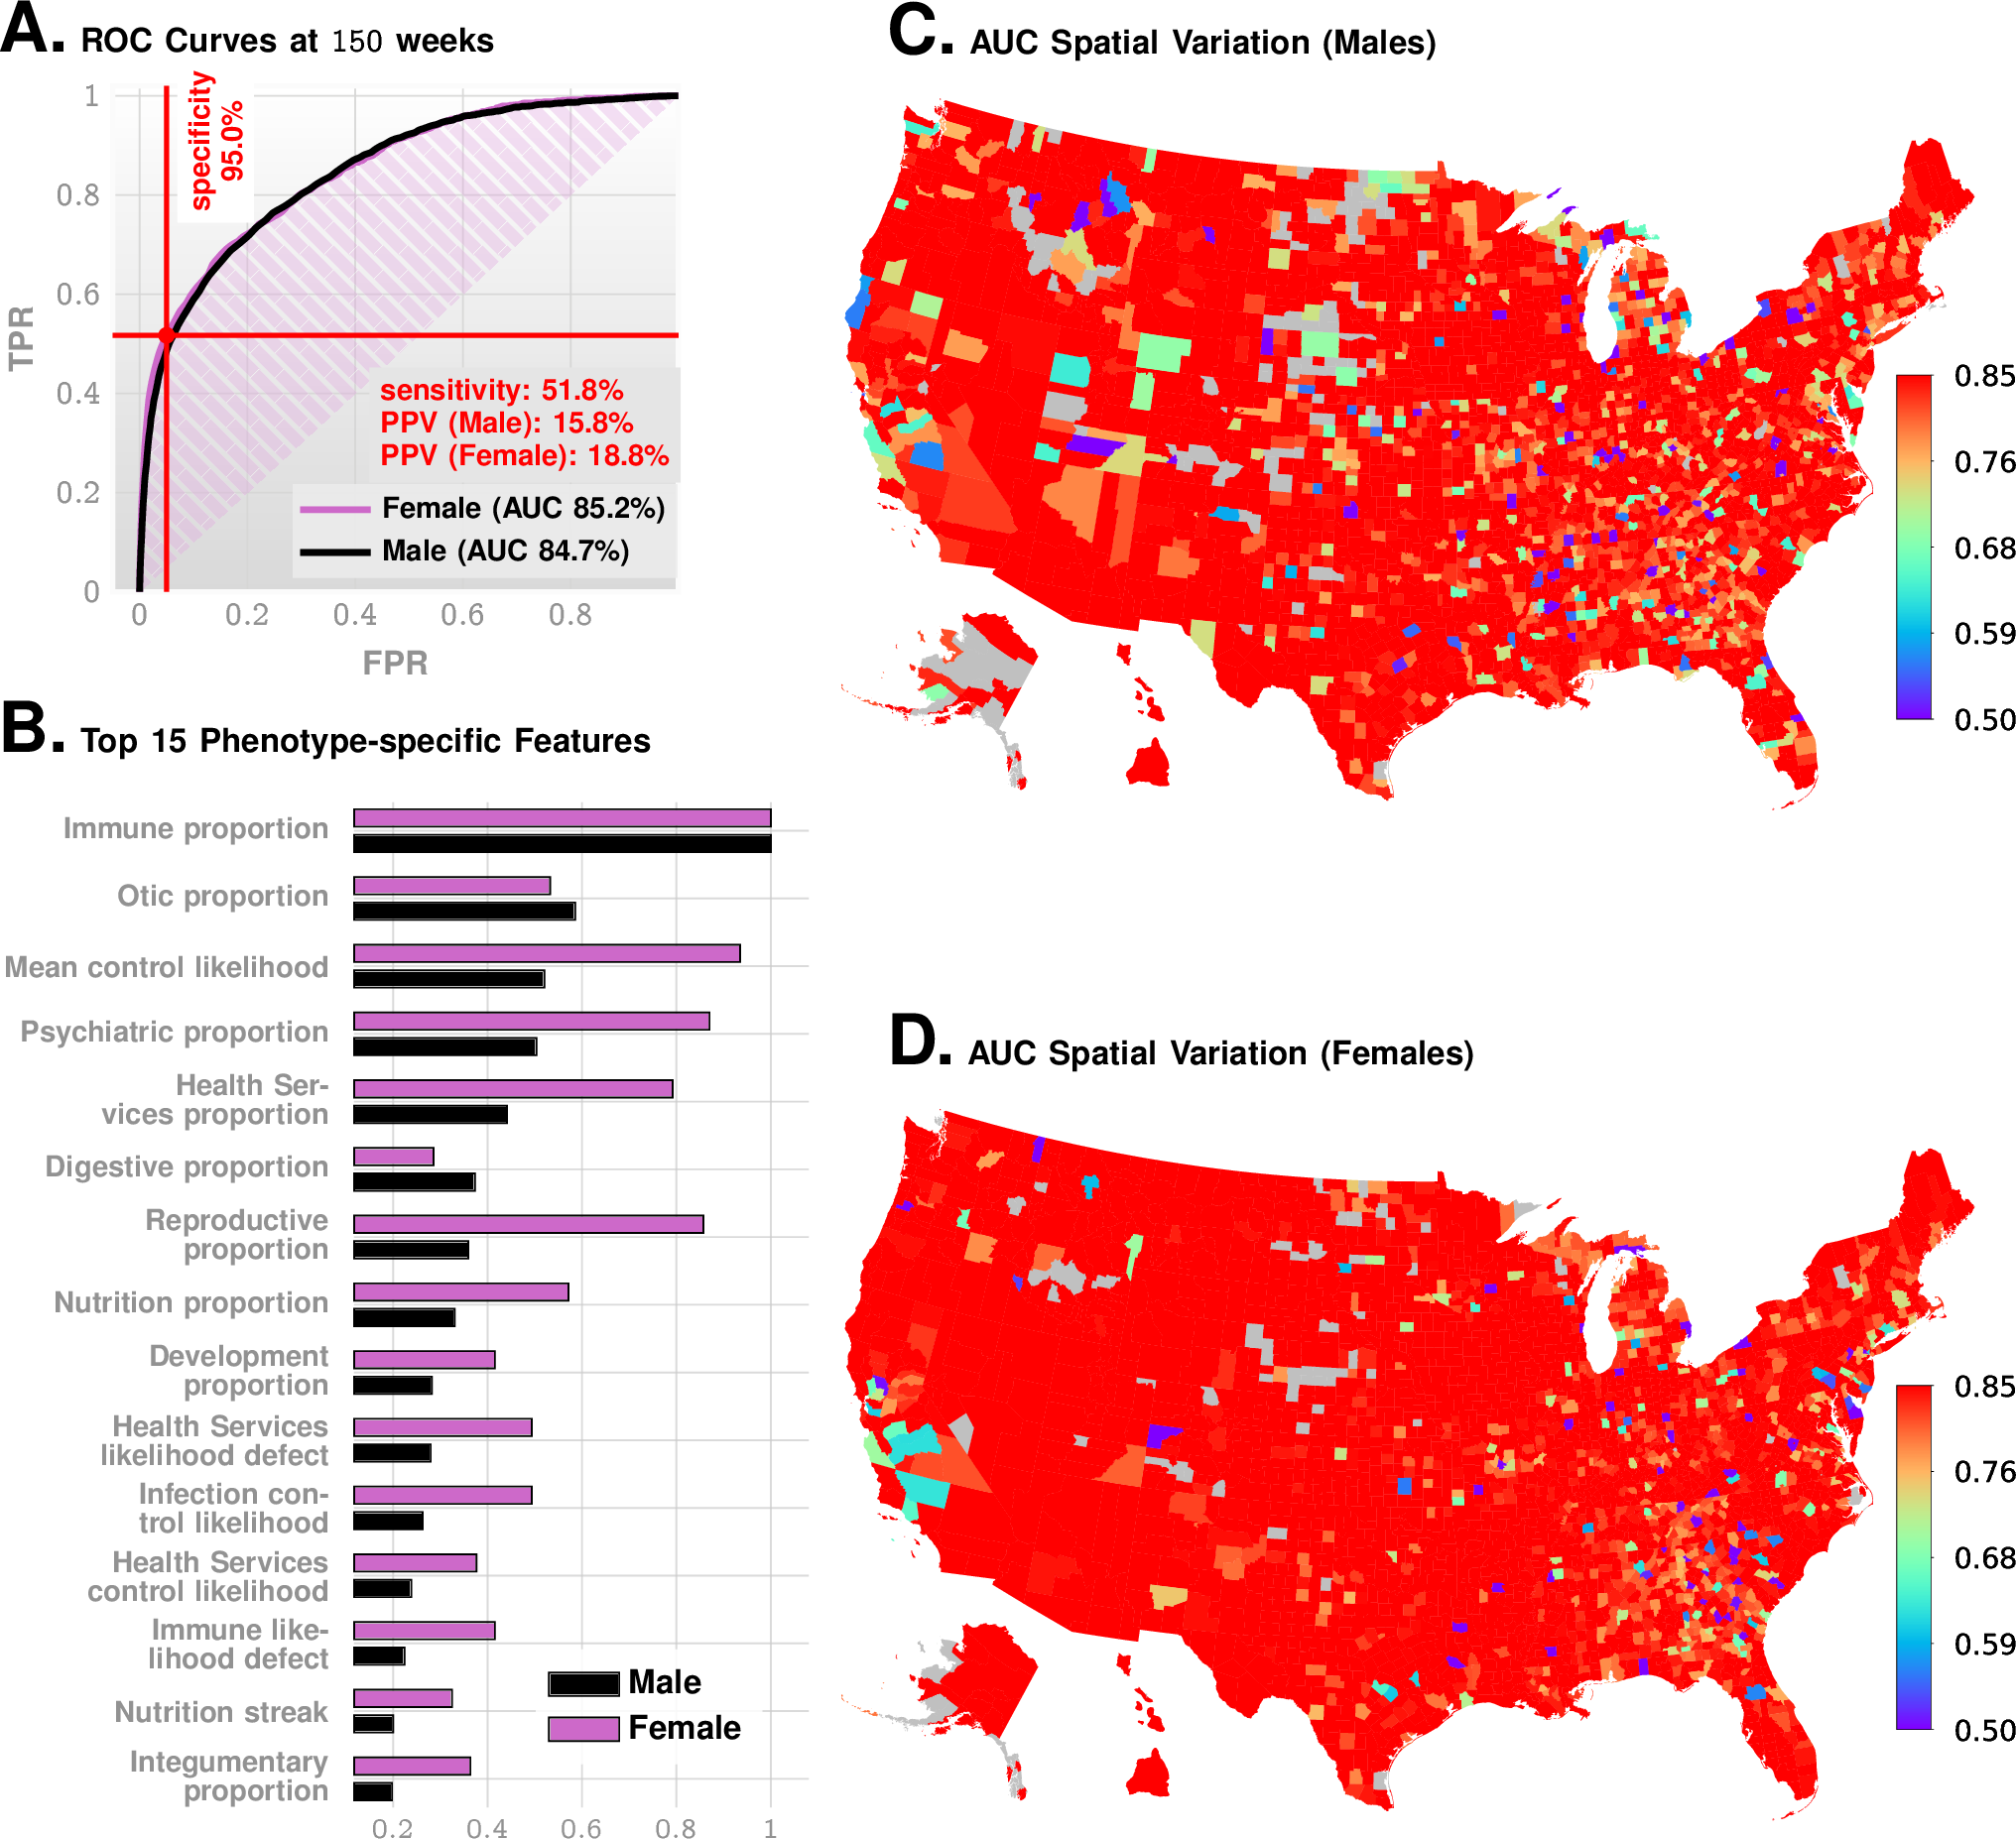
\includegraphics[width=0.9\textwidth]{../results/tex/Figures/External/main2-figure1.pdf}
     \vspace{-15pt}

  \captionN{Predictive Performance. Panel 
       A shows the ROC curves for males and females. Panel B shows the feature importance inferred by our prediction pipeline. The most import feature is related to immunologic disorders, and we note that in addition to features related to individual disease categories, we also have the mean control likelihood (rank 3), which may be interpreted as the average likelihood of the diagnostic patterns correspond to the control category as opposed to the \treatment category. Panels C and D show the spatial variation in the achieved predictive performance at 150 weeks, measured by AUC, for males and females, respectively. Gray areas lack data on either positive or negative cases. Theses county-specific AUC plots show that the performance of the algorithm has  relatively weak geospatial dependence, which is important in the light of current uneven distribution of diagnostic resources.
     }\label{fig1}
        \vspace{-15pt}

\end{figure}
%###########################################################
\subsection{Approach}
The technical approach of this study consists of the development and extension of the \ZERO methodology from our preliminary studies, and application in a primary care setting with view to carrying out objective comparisons between M-CHAT/F and \ZERO. Furthermore, we plan to assess our ability to boost performance from a conditional combination of the two scores.

\paragraph*{Preliminary Studies} We describe the formulation of the \ZERO score, and the underlying principles that distill the estimated risk from EHR databases.
\subsection*{Source of Electronic Patient Records in Preliminary Studies}
Of the two independent sources of clinical incidence data used in our preliminary study,  the primary source used to train our predictive pipeline  is the Truven Health Analytics  MarketScan\textsuperscript{\textregistered} Commercial Claims and Encounters Database for the years 2003 to 2012~\cite{hansen2017truven} (referred to  as the Truven dataset). 
For our analysis, we extracted histories of patients within the age of $0-9$ years, and excluded  patients who do not satisfy the following criteria: 1) At least one code of any available phenotypes is present, 2) Lag between first and last available record for a patient should be at least 15 weeks. These exclusion criteria ensure that we are not considering patients who have too few observations to either train on, or predict outcomes from. 
 For training, we analyzed over 4M children ($n=4.4M$), with 30M diagnostic records (16,649,548 for males and  14,318,303  for females with 9,835 unique diagnostic codes).
%###########################################################
\begin{figure}[!ht]
 % \vspace{-15pt}
  
  \centering 
   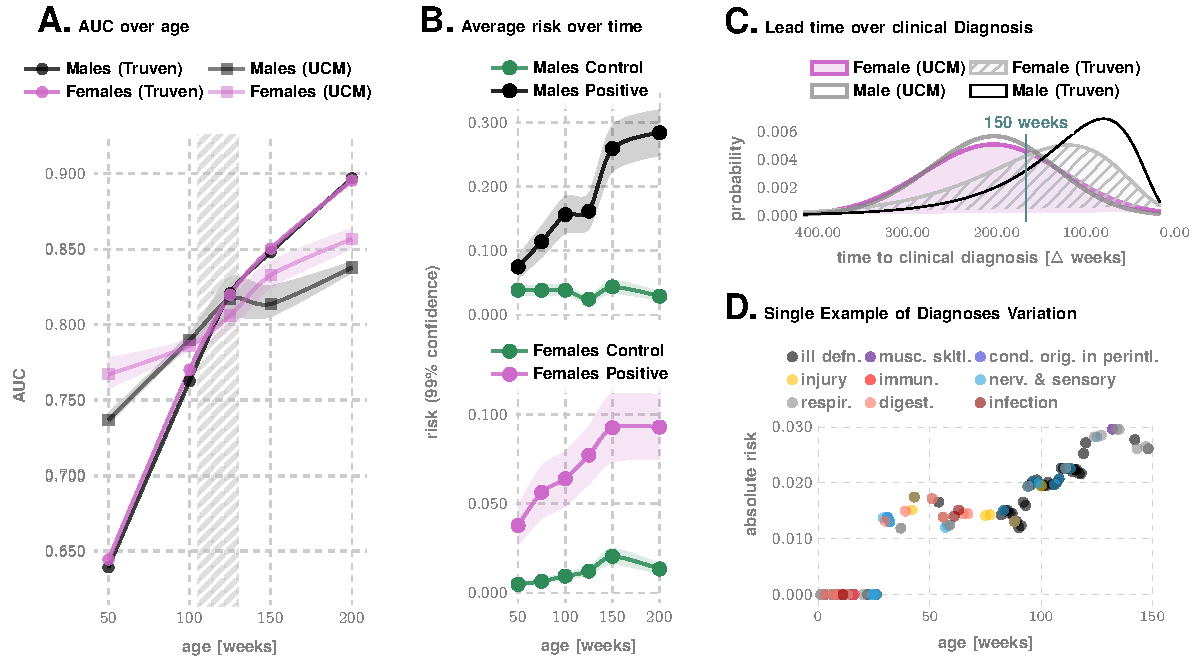
\includegraphics[width=0.9\textwidth]{Figures/test-figure0}
   \vspace{-15pt}

    \captionN{More details on Predictive Performance and Variation of Inferred Risk. Panel A illustrates AUC achieved as a function of
      patient age, for the Truven and UCM datasets. The shaded area outlines the 2 - 2.5  years of age, and  shows that we achieve $>80\%$ AUC for either gender from shortly after 2 years.   Panel B illustrates how the average risk changes with time for the control and the positive cohorts. Panel C shows the distribution of the prediction horizon: the time to a clinical diagnosis after inferred  relative risk crosses $90\%$. Panel d illustrates the risk progression of a specific, ultimately autistic male child in the Truven database. Abbreviations in the legend: ill defn. (Symptoms, Signs, And Ill-Defined Conditions),   musc. skltl. (Diseases Of The Musculoskeletal System And Connective Tissue), cond. orig. in perintl. (Certain Conditions Originating In The Perinatal Period), immun. (Endocrine, Nutritional And Metabolic Diseases, And Immunity Disorders), nerv. \& sensory (Diseases Of The Nervous System And Sense Organs), respir. (Respiratory Disorders), and digest. (Digestive Disorders). %Panel F illustrates  how inferred models differ between the control vs. the \treatment cohorts. On average, models get less complex, implying the exposures get more statistically independent.
    }\label{fig2}
       \vspace{-15pt}

\end{figure}
%###########################################################
\begin{figure*}[t]
  \tikzexternalenable
  \vspace{-10pt}

  \centering
  
  \def\AXISCOL{white}
  \def\TEXTCOL{gray}
   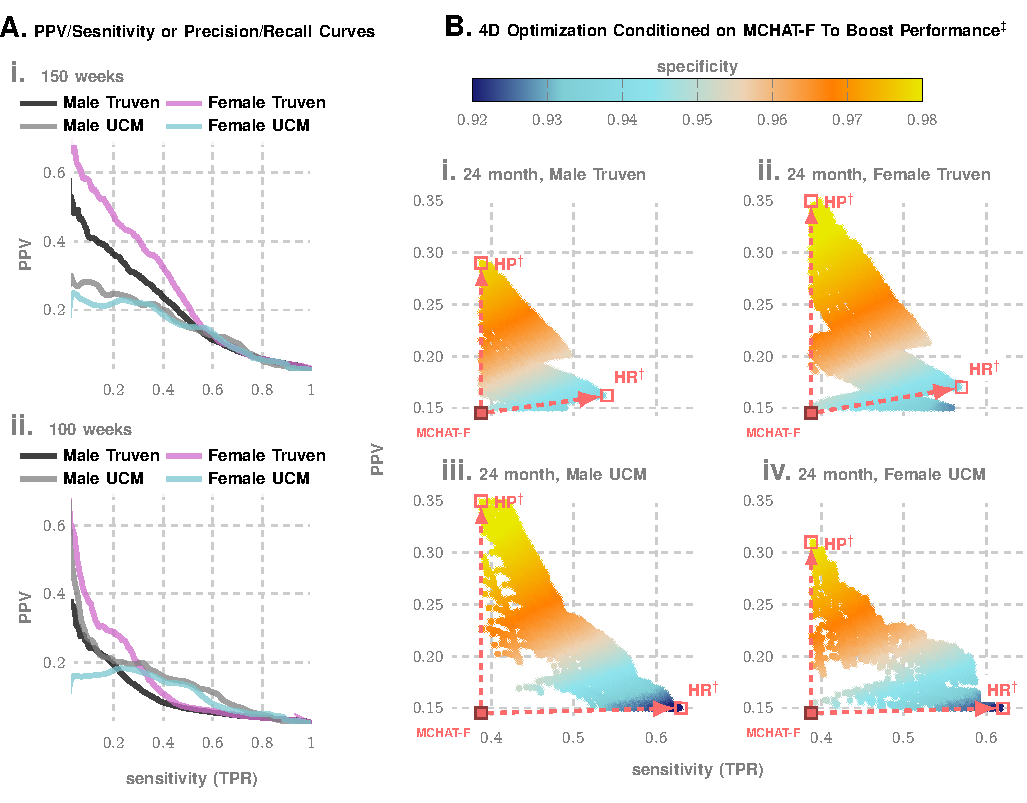
\includegraphics[width=0.8\textwidth]{../results/tex/Figures/External/main2-figure3.pdf}
 % \vspace{0pt}
 %  
\pgfplotsset{
    discard if/.style 2 args={
        x filter/.append code={
            \edef\tempa{\thisrow{#1}}
            \edef\tempb{#2}
            \ifx\tempa\tempb
                \def\pgfmathresult{inf}
            \fi
        }
    },
    discard if not/.style 2 args={
        x filter/.append code={
            \edef\tempa{\thisrow{#1}}
            \edef\tempb{#2}
            \ifx\tempa\tempb
            \else
                \def\pgfmathresult{inf}
            \fi
        }
    }
  }

  \begin{tikzpicture}[font=\bf\sffamily\fontsize{8}{10}\selectfont]
  \def\TEXTCOL{gray}

  \def\DATAPATH{../../revision_results/roc/restricted_neg_len/RAW/}
  \def\datafile{\DATAPATH/thisRFall.csv}


  \def\AXISCOL{white}
  \def\WDTa{1.85in}
  \def\HGTa{2in}
  \def\HGT{1.2in}
  \def\WDT{1.2in}
  \def\MXCOLB{gray}
  \def\FXCOLB{CadetBlue3}
  \def\OPC{.75}
  \def\OPCB{.65}
  \def\LWDT{0.7mm}
  \def\SKIP{4}  
  \def\WDTa{1.75in}
  \def\WDTb{1.25in}
  \def\HGTa{1.65in}
  \def\SKIP{5}
  \def\SKIPB{1}
  \def\LCOL{black}

  \node[] (A0) at (0,0) {};
  \node[anchor=center] (N) at (A0.south)
  {
    \begin{tikzpicture}[text=\TEXTCOL, ]
      \begin{groupplot}
        [name=Agg,
        group style={
          group name=Ag,
          group size=3 by 1,
          xlabels at=edge bottom,
          xticklabels at=edge bottom,
          vertical sep=.75in,
          horizontal sep=.8in,
        },        ,legend cell align={left},
        legend style={anchor=east,at={(-0.12,1.1)},
          inner sep=3pt,
          draw=none,
          fill=white,fill opacity=.850,
          align=left,anchor=west,
          text opacity=1,
          font=\bf\sffamily\fontsize{8}{9}\selectfont,text=black},legend columns=2, 
        name=K,
        clip=true,,
        width=\WDTa,
        height=\HGTa,
        scale only axis=true,
        enlargelimits=false,
        axis on top=false,
        % axis background/.style={
        %   shade,top color=transparent!5,bottom color=transparent!5},
        axis line style={\AXISCOL, opacity=1,ultra  thick, 
          rounded corners=0pt}, 
        grid,
        grid style={thick,dashed, gray!40},
        % xticklabel style={xshift=0.05in,yshift=-.05in},
        xlabel style={yshift=.05in,text=\TEXTCOL},
        ylabel style={align=center,,text=\TEXTCOL,anchor=center,
          yshift=-.15in},
        % tickpos=left,
        ytick align=outside,
        xtick align=outside,
        major tick length=0pt,
        scaled y ticks = false,
        y tick label style={/pgf/number format/fixed,
          /pgf/number format/1000 sep = \thinspace % Optional if you00 separator 
        },
        ylabel={PPV},xlabel={sensitivity (TPR)},point meta=explicit,
        colorbar style={width=.1in,y tick label style={/pgf/number format/fixed,/pgf/number format/precision=2,/pgf/number format/fixed zerofill,
     /pgf/number format/1000 sep = %\thinspace % Optional if you want to replace comma as the 1000 separator 
      },}
        % extra x ticks={1},extra x tick labels={1}
        ]

   \nextgroupplot[colorbar horizontal,xmin=.98,extra x ticks={1},colorbar style={at={(0,1.2)},title={prevalence},title style={yshift=-.1in},
          height=.1in,scaled x ticks=false,
x tick label style={/pgf/number format/fixed,
          /pgf/number format/precision=3,/pgf/number format/fixed zerofill,
          /pgf/number format/1000 sep = %\thinspace % Optional to replace comma as the 1000 separator 
        },
          xticklabel style={yshift=-.025in},},ylabel={MCHAT-F relative wait time},xlabel={MCHAT-F relative sensitivity}]
        \pgfplotsset{
colormap={hot}{color(0cm)=(lightgray!70); color(1cm)=(lightgray!80); color(2cm)=(lightgray!80!Bisque1); color(3cm)=(Bisque1!90!Tomato); color(4cm)=(Tomato); color(5cm)=(Red1)}
}
\addplot [mesh, each nth point=\SKIP, filter discard warning=false, 
        unbounded coords=discard,line width=\LWDT]table [col sep=comma,x=rs,y=tm,meta=rho,
discard if not={gender}{M},
restrict expr to domain={\thisrow{c}}{0.95:1},
restrict expr to domain={\thisrow{rho}}{0.017:0.024},
restrict expr to domain={\thisrow{rs}}{1:1.5},
] {\datafile};   

\node[anchor=west] (x11) at (axis cs:1,0.7) {};
\node[anchor=west] (x12) at (axis cs:1.35,0.525) {};
\node[anchor=west] (xx) at (axis cs:1,0.5) {};


        \nextgroupplot[colorbar,width=\WDTb,xshift=-.2in, title={{\Large i.}  specificity shown by color},colorbar style={xshift=-.1in,,ylabel=specificity,ylabel style={yshift=-.2in}},title style={yshift=.12in,xshift=.15in}]
        \pgfplotsset{
colormap={hot}{color(0cm)=(MidnightBlue); color(1cm)=(CadetBlue2!90!black); color(2cm)=(CadetBlue1!93!black); color(3cm)=(Bisque1!93!black); color(4cm)=(DarkOrange1); color(5cm)=(Yellow2!93!black)}
}

\addplot [mesh, very thick, , each nth point=\SKIPB, filter discard warning=false, 
        unbounded coords=discard
%point meta min=0.92, point meta max=0.98
]table [col sep=comma,x=s,y=p,meta=c,
%discard if not={gender}{M},
restrict expr to domain={\thisrow{c}}{0.966:1},restrict expr to domain={\thisrow{rho}}{0.012:1}] {\datafile};
\node[anchor=west] (x01) at (axis cs:0.5,0.35) {};
\node[anchor=west] (x02) at (axis cs:0.25,0.25) {};

        \nextgroupplot[colorbar,ylabel={},width=\WDTb, title={{\Large ii.}   prevalence shown by color},colorbar style={y tick label style={/pgf/number format/fixed,/pgf/number format/precision=3,/pgf/number format/fixed zerofill,
     /pgf/number format/1000 sep = %\thinspace % Optional if you want to replace comma as the 1000 separator 
      },xshift=-.1in,,ylabel=prevalence,ylabel style={yshift=-.2in}},title style={yshift=.12in,xshift=.15in}]
        \pgfplotsset{
colormap={hot}{color(0cm)=(lightgray!70); color(1cm)=(lightgray!80); color(2cm)=(lightgray!80!Bisque1); color(3cm)=(Bisque1!90!Tomato); color(4cm)=(Tomato); color(5cm)=(Red1)}
}
\addplot [mesh, very thick, each nth point=\SKIPB, filter discard warning=false, 
        unbounded coords=discard]table [col sep=comma,x=s,y=p,meta=rho,
%discard if not={gender}{M},
restrict expr to domain={\thisrow{c}}{0.966:1},restrict expr to domain={\thisrow{rho}}{0.012:1}] {\datafile};

\node[anchor=west] (x1) at (axis cs:0.5,0.35) {};
\node[anchor=west] (x2) at (axis cs:0.25,0.25) {};

      \end{groupplot}
\node[anchor=west, fill=white] (x1) at (x1) {Female};
\node[anchor=center, fill=white] (x2) at (x2) {Male};
\draw[-{Latex},thick,\MXCOL] (x2) -- ($(x2)!.3!(x1)$);
\draw[-{Latex},thick,\FXCOL] (x1) -- ($(x1)!.4!(x2)$);


\node[anchor=west, fill=white] (x01) at (x01) {Female};
\node[anchor=center, fill=white] (x02) at (x02) {Male};
\draw[-{Latex},thick,\MXCOL] (x02) -- ($(x02)!.3!(x01)$);
\draw[-{Latex},thick,\FXCOL] (x01) -- ($(x01)!.4!(x02)$);

\node[anchor=west, fill=white,text=IndianRed1] (x11) at (x11) {CHOP{\color{\TEXTCOL}$^\bigstar$}};
\node[anchor=center, fill=white] (x12) at (x12) {CDC{\color{\TEXTCOL}$^\bigstar$}};
\draw[-{Latex},thick,] (x12) -- ($(x12)!.3!(x11)$);
\draw[-{Latex},thick] (x11) -- ($(x11)!.35!(x12)$);

\draw[-{Latex},very thick,\LCOL]  ($(xx)!1.2in!(xx.north)$) --(xx) node [pos=0,above,right,fill=white,align=center,text=\LCOL,yshift=.1in] {wait-time\\cut in half};

\end{tikzpicture}
  }; 
 \node[anchor=south west] (L1) at ([yshift=-.05in]N.north west) {{\Large C.} Wait time  vs  Recall   (specificity$>97\%$)};
 \node[anchor=south west] (L2) at ([xshift=.4in]L1.south east) {{\Large D.} Pareto fronts for 4D operating point choices wrt prevalence variations};

\node[anchor=north west,align=left,font=\sffamily\fontsize{7}{7}\selectfont] (L3) at (N.south west) {$\ddag$Using population statsitics from CHOP study (See SI-Table~\ref{SI-tabCHOP}). $^\dag$HP: High precision/PPV operating point, HR: High recall/sesitivity operating point \\{\color{\TEXTCOL}$^\bigstar$}CHOP estimates prevalence in its study to be $2.23\%$, while CDC estimates are lower at $1.7\%$};

\end{tikzpicture}

 

 \vspace{-10pt}

 \captionN{\textbf{Metrics relevant to clinical practice: PPV vs Sensitivity trade-offs.} Panel A shows the precision/recall curves, $i.e.$,  the trade-off between PPV and sensitivity. Panel B shows how we can boost performance using population stratification from the distribution of M-CHAT/F scores in the population, as reported by the CHOP study~\cite{pmid31562252}. Panel C illustrates the boosted performance compared to M-CHAT/F alone,
   mesured by the relative percentage increase in sensitivity, and percentage decrease in postive screens. Note that the population prevalence impacts this optimization, and hence  we have  a distinct  curve for each prevalence value ($1.7\%$ is the CDC estimate, while $2.23\%$ is reported by the CHOP study).  The two extreme operating zones marked as High Precision (HP) and High Recall (HR): if we choose to operate in HR, then we do not reduce the number of positive screens by much, but maximize sensitivity, while by operating in HP, we do not increase seinsitivity by much but double the PPV achieved in current practice. Note in all these zones we maintain specificity above $95\%$, which is the current state of art, implying that by doubling the PPV, we can halve the number of positive screens currently reported, thus potentially sharply reducing the queues and wait-times. }\label{figprc}
\end{figure*}
% ###########################################################

While the Truven database is used for both training and out-of-sample cross-validation with held-back patient data, our second independent dataset (referred to as the UCM dataset) consisting of de-identified diagnostic records for children treated at the University of Chicago Medical Center between the years of 2006 to 2018, aids in further cross-validation. We considered children between the ages of $0-5$ years, and  applied the same exclusion criteria as the Truven dataset.

\subsection*{Time-series Modeling of  Diagnostic History}
Individual diagnostic histories  can have long-term memory~\cite{ltgranger80}, implying that the order, frequency, and comorbid interactions between diseases are potentially  important for assessing the future risk of our target phenotype. 
Our  approach to analyzing patient-specific  diagnostic code sequences consists of representing the medical history of each patient as a set of stochastic categorical time-series | one each for a specific group of related disorders |  followed by the inference of stochastic generators  for  these individual data streams. These inferred generators are from a special class of  Hidden Markov Models (HMMs), referred to as Probabilistic Finite State Automata (PFSA)~\cite{CL12g}. The inference algorithm we use is distinct from classical HMM learning, and has important advantages related to the ability to infer structure, and sample complexity. We infer a separate class of models for the \treatment and control cohorts, and then the problem reduces to determining the probability that the short diagnostic history from a  new  patient arises from the \treatment as opposed to the control category of the inferred models. Importantly,  the individual histories are typically short, often have large randomly varying  gaps, and we have no guarantee that model-structural assumptions~\cite{Stoyanov2010,Shumway2000} (linearity, additive noise structure, etc.)  often used in the standard time-series analysis is applicable here. Also, the categorical observations are drawn  from a large alphabet of possible  diagnostic codes, which degrades  statistical power. 

\subsection*{Step 1: Partitioning The Human Disease Spectrum} To address these issues, we begin by partitioning the human disease spectrum into  $17$ non-overlapping  categories, which remain fixed throughout the analysis. Each category is defined by a set of diagnostic codes from the International Classification of Diseases, Ninth Revision (ICD9).
For this study, we considered $9,835$ distinct ICD9 codes (and their ICD10 General Equivalence Mappings (GEMS)~\cite{GEMS} equivalents). We came across 6,089 distinct ICD-9 codes and 11,522 distinct ICD-10 codes in total in the two datasets we analyzed. Transforming the diagnostic histories to report only the broad categories   reduces the number of distinct codes that the pipeline needs to handle, thus improving statistical  power.  The trade-offs for this increased power consist of 1) the loss of distinction between disorders in the same category, and  2) some inherent subjectivity in determining the constituent ICD9 codes that define each category, $e.g.$ an ear infection may be classified either an otic disease or an infectious one.


We do not pre-select the phenotypes; we want our algorithm to seek out the important patterns without any manual curation of the input data. The limitation of the set of phenotypes to $9835$ unique codes arises from excluding patients from the database who have very few and rare codes that will skew the statistical estimates. Next, we process raw diagnostic histories to generate data streams that report only the categories instead of the exact codes. For each patient, his or her  past  medical history is a sequence $(t_1,x_1),\cdots,(t_m,x_m)$, where $t_i$ are timestamps and $x_i$ are ICD9 codes diagnosed at time $t_i$.  We map individual patient history to a three-alphabet  time series $z^k$ corresponding to the disease category $k$,  as follows. For each week $i$,
\cgather{\label{eq1}
  z^k_i =  \left \{ \begin{array}{ll}
                       0 & \textrm{if no diagnosis codes  in week } i\\
                       1 & \textrm{if there exists a diagnosis of category $k$ in week } i\\
                       2 & \textrm{otherwise}
                      \end{array} \right.
                  }The time-series $z^k$ is terminated at a particular week if the patient is diagnosed with ASD the week after. 
In summary, each patient is now represented by $17$ mapped trinary series, which we  use next  to infer population-level PFSA models. 

     

\subsection*{Step 2: Model Inference \& The Sequence Likelihood Defect}
The mapped series, stratified by  gender, disease-category, and ASD diagnosis-status are considered to be independent realizations or sample paths from  relatively invariant stochastic dynamical systems; and we explicitly model these systems as HMMs. We model the \treatment and the control cohorts for each gender, and in  each disease category separately, ending up with a total of $68$ HMMs at the population level ($17$ categories, $2$ genders, $2$ cohort-types: \treatment and control). Each of these inferred models is  a PFSA;  a directed graph with probability-weighted edges, and acts as an optimal generator of the  stochastic process driving the  sequential appearance of the three letters (as defined by Eq.~\eqref{eq1})  corresponding to each gender, disease category, and cohort-type. % These models  are very nearly assumption-free beyond the requirement that  the processes be statistically stationary or slowly varying.  In particular, these models are not  \textit{a priori}  constrained by any structural motifs, complexity, or size, and are   compact representations of  patterns emerging in the mapped time series. Additionally, when learning models for sets of diagnostic histories corresponding to a patient cohort, the histories can be of different lengths.
The modeling objective here is to exploit the relative differences in these  probabilistic  models to reliably infer the cohort-type of a new patient from their  individual sequence  of past diagnostic codes.
%
To that effect, we generalized the well-known notion of Kullbeck-Leibler (KL) divergence~\cite{Cover,kullback1951} between probability distributions to a divergence $\mathcal{D}_{\textrm{KL}}(G \vert \vert H)$ between ergodic stationary categorical stochastic processes~\cite{doob1953stochastic} $G,H$ as:
\cgather{
  \mathcal{D}_{\textrm{KL}}(G \vert \vert H) = \lim_{n\rightarrow \infty} \frac{1}{n}  \sum_{x:|x| = n}p_G(x)\log\frac{p_G(x)}{p_H(x)}  }\noindent
where $\vert x\vert $ is the sequence length, and $p_G(x) ,p_H(x) $ are the probabilities of sequence $x$ being generated by the processes $G,H$ respectively.
Defining the  log-likelihood of  $x$ being generated by a process $G$ as :
\cgather{
    L(x,G)= -\frac{1}{\vert x\vert}\log p_G(x) 
  }\noindent
  The cohort-type for an observed sequence $x$ | which is actually generated by the hidden process $G$ | can be formally inferred from observations based on the following provable relationships:
  \begin{subequations}\label{eqR}\cgather{
    \lim_{\vert x \vert \rightarrow \infty}L(x,G) = \mathcal{H}(G)   \\
    \lim_{\vert x \vert \rightarrow \infty } L(x,H)  =\mathcal{H}(G) +  \mathcal{D}_{\textrm{KL}}(G \vert \vert H)   
    }\end{subequations} where  $\mathcal{H}(\cdot)$ is the entropy rate of a process~\cite{Cover}. Importantly, Eq.~\eqref{eqR} shows that the computed likelihood has an additional non-negative contribution from the divergence term, when we choose the incorrect generative process.  Thus, if a  patient is eventually going to be diagnosed with ASD, then we expect that the disease-specific mapped series corresponding to  her diagnostic history be modeled by the PFSA in the \treatment cohort. Denoting the PFSA corresponding to disease category $j$ for \treatment and control cohorts as $G^{j}_+,G^{j}_0$ respectively, we can compute the \textit{sequence likelihood defect} (SLD, $\Delta^j$) as:
    \cgather{
      \Delta^j \triangleq L(G^{j}_0,x) - L(G^{j}_+,x) \rightarrow \mathcal{D}_{\textrm{KL}}(G^{j}_0 \vert \vert G^{j}_+) \label{eq6}
      }With  the inferred population-level PFSA  models and  the individual diagnostic history, we can now estimate the SLD measure on the  right-hand side of Eqn.~\eqref{eq6}. The higher this likelihood defect, the higher  the similarity of the patient's history  to ones that have an eventual ASD diagnosis with respect to the disease category being considered. SLD is the core novel analytic tool used in this study  to tease out  information relevant to the risk estimator and is key to the design of our risk estimation pipeline.

\subsection*{Step 3: Risk Estimation Pipeline With Semi-supervised \& Supervised Learning Modules}
Ultimately, the risk estimation pipeline operates on patient specific information limited to the
gender and available  diagnostic history from birth, and produces an estimate of the relative risk of ASD diagnosis at a specific age, with an associated  confidence value.
To learn the parameters and associated model structures of  this pipeline, we transform the patient specific data to a set of engineered features, and the feature vectors realized on the
\treatment and control sets are then used to train a gradient-boosting classifier~\cite{gbm02}. Of the set of engineered features, the most important are the  disease-category-specific SLD described above. For example, if $SLD > 0$ for a specific patient for every disease category, then he or she is likely to have an ASD diagnosis eventually. However, not all disease categories are equally important for this decision; parametric  tuning of the classifier allows us to infer the optimal combination weights, as well as compute the relative risk  with associated confidence. In addition to category-specific SLDs, we use a range of other derived quantities as features, including the mean and variance of the defects computed over all disease categories, the occurrence frequency of the different disease groups, etc. 
The top $15$ features used in our pipeline may be ranked in order of their relative importance (See Fig.~\ref{fig1}B), by estimating the loss in performance when dropped out of the analysis, and the importance of  infections and immunologic disorders are clearly evident (See Fig.~\ref{fig1}B).  

% PFSA : TRAIN : TEST ratio ::: [.2, .256, .544]
% [*M*]
% Total size : 2.94M
% Set sizes: 590k, 750k, 1.6M
% [*F*]
% Total size : 2.75M
% Set sizes: 550k, 700k, 1.5M
%\subsection*{Receiver Operating Characteristic \& Relative Risk Calculation}
\subsection*{Calculating Relative Risk}
Our pipeline maps medical histories to a  score, which is interpreted as a raw indicator of 
risk | higher this value, higher the probability of a future diagnosis. However, to make crisp predictions, we must choose  a decision threshold for this raw score. Conceptually identical to the notion of Type 1 and Type 2 errors in classical statistical analyses, the choice of a threshold trades off false positives (Type 1 error) for false negatives (Type 2 error): choosing a small threshold  results in predicting a larger fraction of future diagnoses correctly, $i.e.$ have a high true positive rate (TPR), while simultaneously suffering from a higher false positive rate (FPR), and vice versa.
We choose thresholds for the standalone \ZERO method by  maximizing the $F_1$-score, defined as the harmonic mean of sensitivity and specificity, to make a   balanced trade-off between the two kinds of errors.
%
The \textit{relative risk} is then defined as the ratio of the raw pipeline score to the chosen decision threshold. While the raw score does not give us  actionable information,  the relative risk being close to or greater than 1.0 for a specific child signals the need for intervention.
%
\subsection*{Standalone Predictive Performance}
% %####################################
\def\RCOL{\rowcolor{teal!40}}
%#################################### 
\begin{table}[t]   
\centering 
\captionN{Standalone \ZERO PPV Achieved}\label{tabssp}
\footnotesize
\mnp{\textwidth}{%\vskip .1em
\vspace{-15pt}

\scriptsize (For Comparison M-CHAT/F Performance:  sensitivity=$38.8\%$, specificity=$95\%$, PPV=$14.6\%$ between within 26 months ($\approx$112 weeks))\\
\vskip .1em}
%
%
\begin{tabular}{L{.75in}|L{.75in}|L{.75in}|L{.5in}|L{.5in}|L{.75in}}
\hline
week&spec.&sens.&PPV&sex&dataset\\\hline
100&0.92&0.39&0.14&F&UCM\\\hline
100&0.95&0.39&0.19&M&UCM\\\hline
100&0.93&0.39&0.13&F&Truven\\\hline
100&0.91&0.39&0.10&M&Truven\\\hline
%\RCOL 112&0.94&0.35&0.17&F&UCM\\\hline
\RCOL 112&0.93&0.39&0.16&F&UCM\\\hline
\RCOL 112&0.95&0.39&0.20&M&UCM\\\hline
\RCOL 112&0.96&0.39&0.22&F&Truven\\\hline
\RCOL 112&0.95&0.39&0.17&M&Truven\\\hline
% 150&0.94&0.39&0.19&F&UCM\\\hline
% 150&0.98&0.39&0.34&F&Truven\\\hline
% 150&0.97&0.39&0.26&M&Truven\\\hline
% 150&0.97&0.39&0.26&M&UCM\\\hline

\end{tabular}
\end{table}  
%####################################
% %####################################
The standalone performance of our risk estimator is summarized  in Fig.~\ref{fig1} and Fig.~\ref{fig2}. The task of predicting if a patient has a future ASD diagnosis, at an earlier date compared to the clinical diagnosis,  may be viewed as a binary classification problem.
In our case, we achieve an out-of-sample AUC of $82.3\%$ for males and $82.5\%$ for females at $125$ weeks of age for the Truven dataset. In the UCM dataset, our performance is comparable: $83.1\%$ and $81.3\%$ for males and females respectively at $125$ weeks of age. The good agreement of the out-of-sample performance on these independent datasets lends strong evidence for the claims made in this study. The specificity, sensitivity, PPV trade-offs are shown in Table~\ref{tabssp}.


We enumerate the top $15$ predictive features in Fig.~\ref{fig1}B. 
We also computed the county-specific performance of the risk pipeline for the Truven dataset, and we got nearly uniform performance across the country for both genders, with the exception of  few isolated counties lacking patients in the appropriate age groups (See Fig.~\ref{fig1}, panels C and D) which prevented us from estimating AUC for those counties. Thus the performance of the algorithm is relatively agnostic to the number of local diagnoses, which is import in light of the fact that   crucial diagnostic resources currently have a very uneven distribution (only 7\% of developmental pediatricians practice in rural areas, and some states in US do not even have a developmental pediatrician~\cite{gordon2016whittling,althouse2006pediatric}).


Fig.~\ref{fig2}A illustrates the variation of the  AUC  with increasing age of the subjects plotted with 99\% confidence bounds: the increase is very nearly  linear, with a change of gradient near the $150$ week mark. We suspect that the median diagnosis age in the databases ($\approx 150$ weeks) manifests this inflection. The curves for the smaller UCM dataset are less smooth, probably due to more uncertainty. We find that while the AUC gradients are different in the two datasets, they tend to match up in later ages. The differences in the early ages are possibly due to differences in patient statistics: a larger number of patients in Truven at the earlier ages with a relatively smaller number of observations on average.

We plot the absolute or raw risk over time for males and females for the out-of-sample control and \treatment cohorts in Fig.~\ref{fig2}B. We see that while the risk for the control cohort remains more or less stable,   that for the \treatment cohort rapidly increases. Notably, in these risk plots, averaged over the population,   we see disambiguation  early, right from $50$ weeks. Also, we see a saturation of the risk after $150$ weeks, which corresponds to the median diagnosis age in the database (approx. 150 weeks). Thus, if a child is not diagnosed up to that age, then the  risk  falls, since the probability of a diagnosis in the population starts to go down after this age.

\subsection*{Calculating PPV, Sensitivity \& Specificity Trade-offs \& M-CHAT/F Comparison}
The sensitivity vs PPV plots, also known as the precision-recall curves (See Fig.~\ref{figprc}A) are constructed in a similar fashion as the ROC curves by varying the decision threshold. These curves  allow direct comparison with the  state of the art screening tests,$e.g.$, M-CHAT/F, in a manner that is most relevant to clinical practitioners.
%
Guthrie $\etal$~\cite{pmid31562252} from Children's Hospital of Philadelphia (CHOP) has recently demonstrated that when applied as a nearly universal screening tool, M-CHAT/F has a sensitivity of 38.8\%, specificity of 94.9\% and PPV of 14.6\%, implying that out of every 100 children who in fact ave ASD, the M-CHAT/F flags about 39, and out of every 100 children it flags, about 85 are false positives. The PPV is affected by the prevalence of the disease. This work is the only large-scale study of M-CHAT/F (n=20,375) we are aware of with sufficient follow-up after the age of four years to provide a reasonable degree of confidence in the reported performance values.

Comparing the performance metrics achieved at different age groups across data sets and genders for our pipeline (See Table~\ref{tabssp}), we conclude that our approach produces a strictly superior PPV (exceeding M-CHAT/F PPV by at  $14\%$ (14.1-33.6\%) when sensitivity and specificity are held at comparable values around the age of 26 months ($\approx 112$ weeks). We cannot compare at other operating points due to a lack of M-CHAT/F performance characterization anywhere else.
%###############################################
\begin{table}[t]
  \centering

  \captionN{Population Stratification Results on large M-CHAT/F Study(n=20,375)  reproduced from Guthrie $\etal$~\cite{pmid31562252} }\label{tabCHOP}
\footnotesize
  \begin{tabular}{C{.65in} | L{1.5in}|L{1.5in}|L{1in}|L{1in}||L{.55in}}\hline
 \bf \sffamily   Id &  \bf \sffamily Sub-population & \bf \sffamily Test Result & \bf \sffamily ASD pos. & \bf \sffamily ASD Neg. & \bf \sffamily Total \% \\\hline
   A &  M-CHAT/F $\geqq 8$ & Positive & 0.34\% & 0.64\% & 0.99\% \\\hline
  B &   M-CHAT/F $\in [3,7]$ & Positive (follow-up)& 0.52\% & 4.39\% & 4.91\% \\\hline
 C &    M-CHAT/F $\in [3,7]$ & Negative (follow-up)& 0.14\% & 3.1\% & 3.24\% \\\hline
  D &   M-CHAT/F $\in [0,2] $ & Negative & 1.22\% & 89.63\% & 90.86\% \\\hline\hline
    Total \%& &   &2.23\% & 97.77\% & 100\% \\\hline
    \end{tabular}
\end{table}
%###############################################
\subsection*{Boosting Performance Via Leveraging Population Stratification Induced By M-CHAT/F}
In this study, we leverage the population stratification induced by an existing independent screening test (M-CHAT/F) to improve combined performance. Here a combination  refers to the conditional choice of the sensitivity/specificity trade-offs for our tool in each sub-population such that the overall performance is optimized with respect to whether we wish to maximize the PPV or the sensitivity at a specified minimum level of specificity. Assume that there are $m$ sub-populations such that:
the sensitivities, specificities achieved, and the prevalences in each sub-population are given by $s_i,c_i$ and $\rho_i$ respectively, with $ i \in \{1,\cdots, m\}$. Let $\beta_i$ be the relative size of each sub-population. Then, we can show:
\begin{subequations}\label{eqscpop}
\cgather{
  s= \sum_{i=1}^m s_i \gamma_i  , \textrm{ and } 
  c= \sum_{i=1}^m c_i \gamma_i' %\\PPV = \frac{s}{s+(1-c)(\frac{1}{\rho} -1)}
\textrm{ where we have denoted: }
\gamma_i = \beta_i \frac{\rho_i }{\rho}, \textrm{ and }  \gamma_i'= \beta_i \frac{1-\rho_i}{1-\rho}
  }%
\end{subequations}%
and $s,c,\rho$ are the overall sensitivity, specificity, and prevalence.
Knowing the values of $\gamma_i, \gamma_i'$, we can carry out an $m$-dimensional search to identify the feasible choices of $s_i,c_i$ pairs for each $i$, such that some global constraint is satisfied, $e.g.$ minimum values of specificity, sensitivity, and PPV. We consider  $4$ sub-populations defined by M-CHAT/F score brackets~\cite{pmid31562252}, and if the screen result is considered a positive (high risk, indicating the need for a full diagnostic evaluation) or a negative, $i.e. $, low risk: 1) score   $\leq 2$  screening ASD negative, 2) score $[3-7]$ screening ASD negative on follow-up, 3) score  $[3-7]$ and  screening ASD positive on follow-up, and 4) score  $\geq 8$,  screening ASD positive. (See Table~\ref{tabCHOP}). The ``follow-up'' in the context of M-CHAT/F refers to the re-evaluation of responses by qualified personnel. We use published data on the relative sizes and the prevalence statistics in these sub-populations~\cite{pmid31562252} to   compute the feasible conditional choices of our  operating point  to strictly supersede  M-CHAT/F performance. Two limiting operating conditions are  of special interest here, where we maximize PPV under some minimum specificity and sensitivity (denoted as  the High Precision or the HP operating point), and where we maximize sensitivity under some minimum PPV and specificity (denoted as the High Recall or the HR  operating point). Taking these minimum values of specificity, sensitivity, and PPV to be those reported for  M-CHAT/F, we identify the set feasible set of conditional choices in a four dimensional decision space  that would  outperform M-CHAT/F in universal screening. 

%#################################### 
\begin{table}[t]
\centering
\captionN{Boosted Sensitivity, specificity and PPV Achieved at  26 months Personalized Operation Conditioned on M-CHAT/F Scores}\label{tabboost}
\footnotesize
\begin{tabular} {L{.35in}|L{.35in}|L{.35in}|L{.35in}||L{.35in}|L{.35in}|L{.375in}||L{.375in}|L{.35in}|L{.35in}||L{.6in}}
\hline
\multicolumn{4}{c||}{\cellcolor{lightgray!60}M-CHAT/F Outcome}  & \multicolumn{3}{c||}{\mnp{.9in}{\vskip .2em global performance (Truven)\vskip .2em  } }&\multicolumn{3}{c||}{\mnp{1in}{\vskip .2em global performance\\(UCM)\vskip .2em }} &  \multirow{3}{*}{prevalence$^\star$}\\\cline{0-9}
 0-2  NEG & 3-7  NEG & 3-7  POS & $\geq  8$  POS & \multirow{2}{*}{\mnp{.1in}{speci-ficity}} & \multirow{2}{*}{\mnp{.1in}{sensi-tivity}} &\multirow{2}{*}{PPV}& \multirow{2}{*}{\mnp{.1in}{speci-ficity}} & \multirow{2}{*}{\mnp{.1in}{sensi-tivity}} & \multirow{2}{*}{PPV} & \\\cline{0-3}
\multicolumn{4}{c}{\cellcolor{lightgray} specificity choices}  & & & &&&&\\\hline 
  0.48&0.87&0.97&0.99&0.98&0.432&0.331&0.98&0.355&0.289\\\hline 
0.38&0.54&0.94&0.98&0.95&0.736&0.203&0.95&0.628&0.178\\\hline  
\end{tabular}
\vskip 1em

\flushleft
$^\star$Prevalence reported by CDC is $1.7\%$, while the CHOP study reports a value of $2.23\%$. Results depend on the prevalence estimate.
\end{table}  
%####################################


This ultimately yields an overall performance significantly  superior to  M-CHAT/F alone.
We carry out a four dimensional search at the age of 26 months ($\approx 112$ weeks) to  identify the feasible region with  PPV  $>14.6\%$ and sensitivity  $>38.8\%$ simultaneously while keeping specificity  $>94\%$. These four  dimensions reflect the independent choice of sensitivities in the corresponding sub-populations. For each set of  choices, the associated  specificities are read-off from our fixed pre-computed ROC curve corresponding to $112$ weeks, and then the overall sensitivity, specificity and PPV are calculated using standard relationships.

We get a PPV close to or exceeding $30\%$ at the high precision (HP) operating point across datasets ($>33\%$ fro Truven, $>28\%$ for UCM), or a sensitivity close to or exceeding $50\%$ for the high recall (HR) operating point ($>58\%$ for  Truven, $>50\%$ for UCM), when we restrict specificities to above $95\%$ (See Table~\ref{tabboost}). 
  
It is important to compare these results directly with M-CHAT/F performance, as shown in Fig.~\ref{figprc}, panels C. In panel C, we show that for any stable population prevalence between 
$1.7\%$ and $2.23\%$, the conditional operation can achieve  double the PPV relative to M-CHAT/F alone without losing sensitivity at $>98\%$ specificity, or increase the sensitivity by $\sim 50\%$ without sacrificing PPV and   not letting the  specificity to drop below $94\%$.
%These results are for the Truven dataset, but the UCM results are similar.
%

Importantly, designing  rules for  conditional  operation  only requires average population characteristics, $i.e.$, an  estimate of ASD prevalence in the sub-populations defined by the  relevant brackets of M-CHAT/F scores, and the prevalence of these score brackets in the general population. In particular,   M-CHAT/F scores of individual patients are unnecessary for designing the rules themselves, or evaluating the overall expected performance in the population, provided the stratification statistics (Table~\ref{tabCHOP}) remains invariant. However, in the proposed study, we will be able to compute explicit dependency relationships between M-CHAT/F and \ZERO scores.
%

\subsection*{Inferred Co-morbidity Patterns \& Normalized Prevalence Comparison}
% ###########################################################

\begin{figure*}[t]
  \tikzexternaldisable
  \vspace{-10pt}

  \begin{tikzpicture}[font=\bf\sffamily\fontsize{8}{8}\selectfont,scale=.7]
    \node[label={[yshift=-.5in]90:{\Large A.} Males}] (A) at (0,0) {
      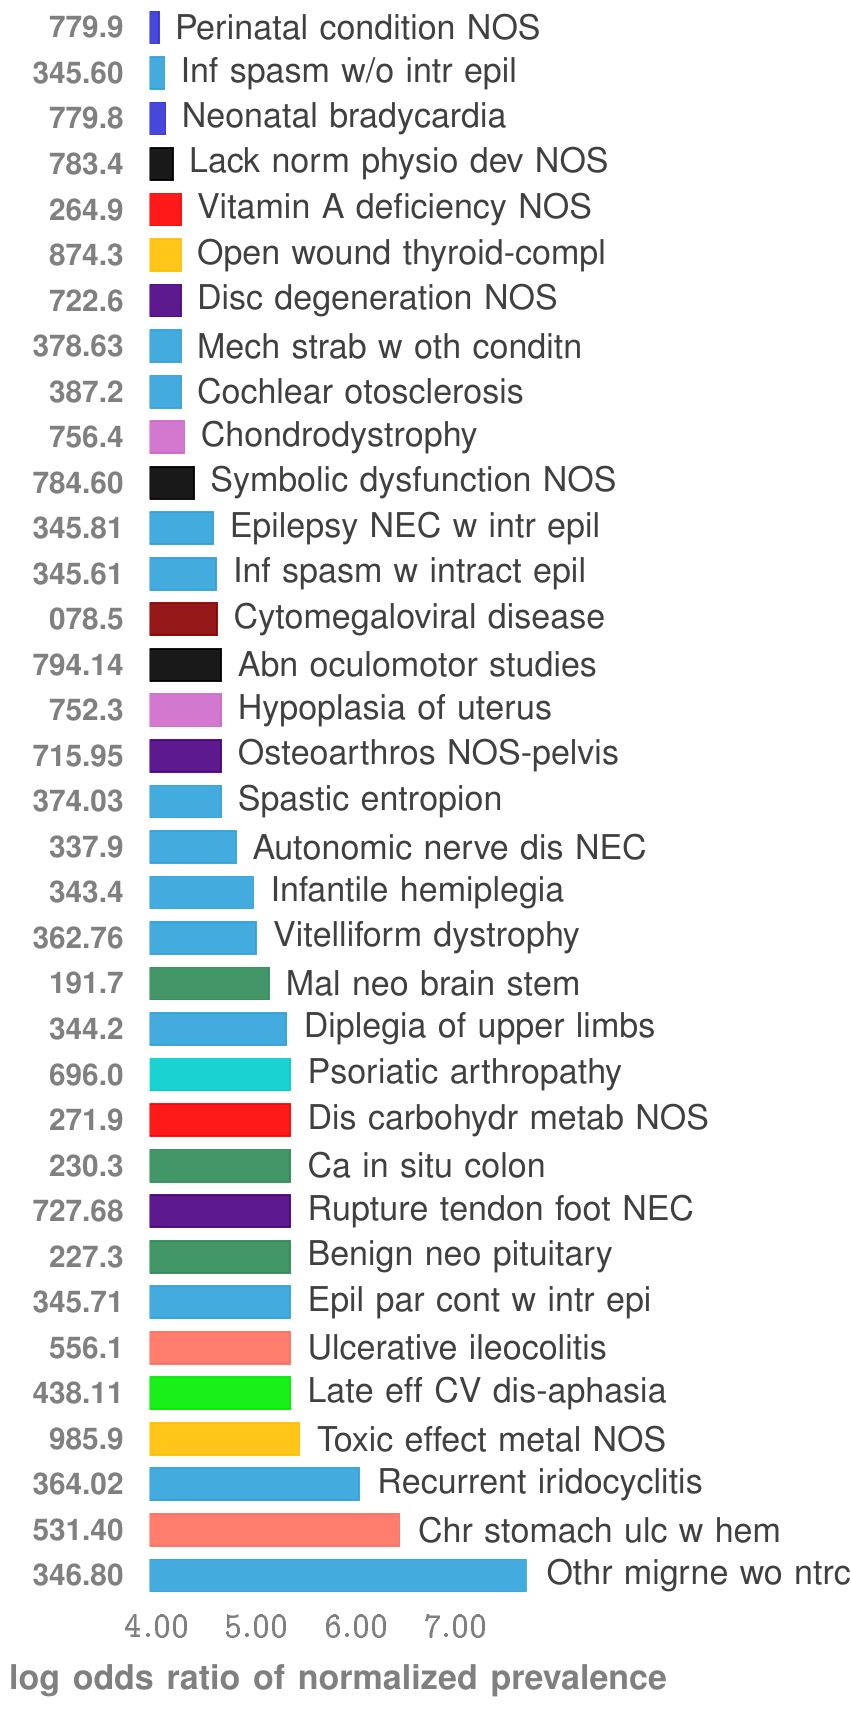
\includegraphics[height=6in,angle=90]{Figures/bars1}};
    \node[anchor=west] (B) at (A.east) {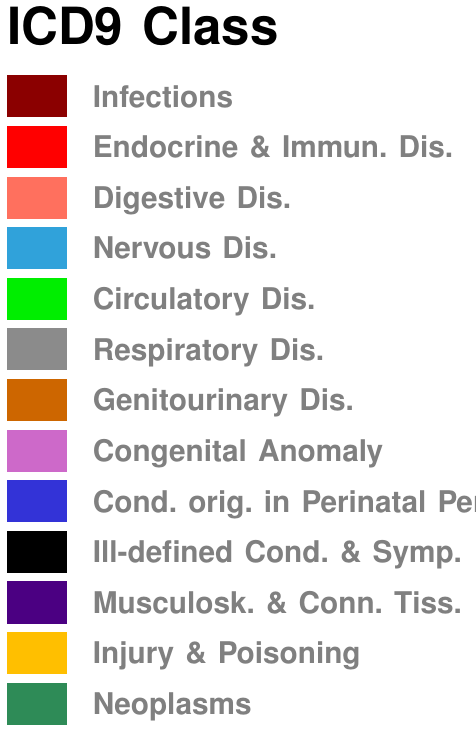
\includegraphics[height=2in,angle=0]{Figures/bars2}};
  \end{tikzpicture}
  \vspace{-10pt}
  
  \captionN{Difference in occurrence frequencies of diagnostic codes between true positive (TP) and true negative (TN) predictions in males. The color coding shows the disease categories of the co-morbidities.}\label{fig3}
\end{figure*}
% ###########################################################
The predictive ability of our pipeline arises from the difference in patterns of co-morbid disorders between the \treatment and the control cohorts: the diagnostic history of individual patients is not random and hides key signatures to future neuropsychiatric outcomes. As an illustrative example, a single random patient from the Truven database is illustrated in Fig.~\ref{fig2}D. Color-coding the diagnoses according to the broad ICD9 disease categories reveals that for this specific individual, infections and immunological disorders are experienced early to a much higher degree compared to other diseases, and diseases of the nervous system and sensory organs, as well as ill-defined symptoms dominate the latter period. This suggests the necessity of a deeper interrogation of the structure of co-morbid patterns, which we carried out in our preliminary investigations, as described next.

While the ASD co-morbidity burden  is reported to be high for nearly the entire spectrum of  physiological disorders, in our preliminary we find novel association patterns in normalized prevalence | the odds of experiencing a specific disorder, particularly in the early years (age~$<3$ years), normalized over all unique disorders experienced in the specified time-frame. Additionally, we only focus on  the true positives in the \treatment cohort and the true negatives in the control cohort. This  allows us to investigate  patterns that correctly disambiguate future ASD status, $i.e.$, strongly favor one outcome over the other at the individual level (as opposed to population-level prevalence rates), as shown in  Fig.~\ref{fig3} for males.

Additionally, we found in our preliminary studies indications of : 1) \textit{negative associations:} there are diseases that are negatively associated with ASD diagnosis with respect to normalized prevalence, $i.e.$, having those codes over-represented relative to other codes in one's diagnostic history favors ending up in the control cohort, 2) \textit{gendered impact:} there are gender-specific differences in the impact of specific disorders which will be further investigated in this study.
%
\subsection*{Effect of Change In Diagnostic Criteria: Inclusion of PDD \&  Asperger's Syndrome}
%
The DSM-5 established a single category of ASD to replace
the subtypes of autistic disorder,
Asperger syndrome, and pervasive
developmental disorder not
otherwise specified in the Diagnostic
and Statistical Manual of Mental
Disorders, Fourth Edition, Text
Revision (DSM-IV-TR)~\cite{hyman2020identification}. This aligns with our use of diagnostic codes from ICD9 299.X as specification of an ASD diagnosis, and use GEMS mapping to 299.X from ICD10 codes when we encounter them.
Importantly, we found that it is  difficult to design a high performing pipeline that recognizes these ASD sub-types separately, even if we so wanted.
%
\subsection*{Disambiguation From Unrelated Psychiatric Phenotypes}
%
 We will investigate  discrimination between ASD and  unrelated psychiatric phenotypes. In our preliminary studies, we  investigated this by restricting the  control  cohort in validation to  patients with at least one non-ASD psychiatric code, annd obtained  high discrimination reaching AUCs over $90\%$ at $100-125$ weeks of age, suggesting that our pipeline is  mostly specific to ASD.
%
\subsection*{Sanity Checks: Uncertainty in EHR Records \& Baseline Approaches in Machine Learning}
Recent changes in diagnostic practice, $e.g.$ increased diagnoses from individual clinicians versus prior eras that only allowed diagnosis from the gold-standard multi-disciplinary teams can  increase observed   prevalence, and  raises the possibility that  some diagnostic codes pertaining to ASD in medical history databases could be arising from less restrictive workflows, and  are susceptible to increased uncertainty.  In our study, we verified that restricting the \treatment cohort to children with at least two  distinct ASD diagnostic codes in their medical histories instead of one, has little impact on  out-of-sample predictive performance.
 
We  verified that class imbalance is not inappropriately  enhancing our performance, by replacing  the  control cohort with a random sample of size equal to that of the \treatment cohort in out-of-sample tests.

We also found that the density of diagnostic codes in a child's medical history by itself is somewhat predictive of a future ASD diagnosis, but not at clinically significant levels.



\begin{figure}[t]
\begin{center}
\tikzexternaldisable
\begin{tikzpicture}
  \def\CGOL{lightgray}
  \def\FCOL{Green1}
  \tikzstyle{ann} = [draw=,fill=\CGOL,text width=.75in,anchor=north,align=center]
  \tikzstyle{mls} = [circle,shading=ball,anchor=center, fill=Red1, draw=black, text width=.15in, align=center,inner sep=0pt, very thick,text=white]


  \node[] (P0) at (0,0) {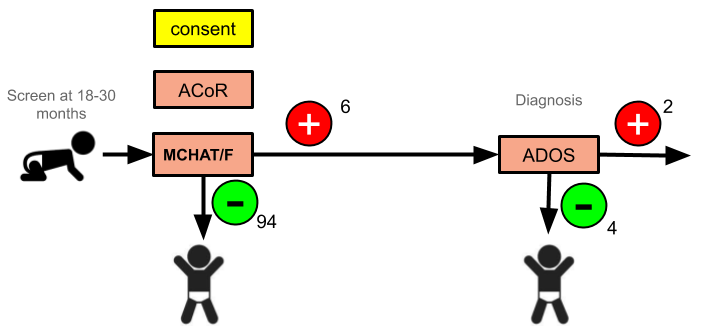
\includegraphics[width=6in]{Figures/value}};

  \end{tikzpicture}
\end{center}
\vspace{-10pt}

\captionN{\textbf{Patient flow logic.} Consenting families with children between 18 to 30 months are subjected to both M-CHAT/F and \ZERO screens, and those with a MCHAT-F flag is scheduled for an ADOS evaluation for ascertaining ASD status. Note that by our calculations, for every 100 children, we expect to 6 MCHAT-F flags, out of which 4 on average will get a negative diagnosis by ADOS.}\label{figflow}
\end{figure}

% \begin{figure}
% \begin{center}
% \tikzexternaldisable
% \begin{tikzpicture}
%   \def\CGOL{lightgray}
%   \def\FCOL{Green1}
%   \tikzstyle{ann} = [draw=,fill=\CGOL,text width=.75in,anchor=north,align=center]
%   \tikzstyle{mls} = [circle,shading=ball,anchor=center, fill=Red1, draw=black, text width=.15in, align=center,inner sep=0pt, very thick,text=white]


%   \node[ann,fill=gray] (P0) at (0,0) {Patient\\Consent};

%   \node[ann,fill=gray,anchor=west] (M) at ([xshift=.45in,yshift=.5in]P0.east) {M-CHAT/F};
%   \node[ann,fill=gray,anchor=west] (Z) at ([xshift=.45in,yshift=-.5in]P0.east) {\ZERO};

%   \node[ann,fill=gray,anchor=west] (A) at ([xshift=1.75in]P0.east) {ADOS};
%   \node[ann,fill=gray,anchor=west] (D) at ([xshift=3in]P0.east) {ASD\\Diagnosis};
%   \draw[-{latex},ultra thick] ([xshift=-.75in]P0.west) -- (P0.west);
%   \draw[-{latex},ultra thick] ([xshift=0in]P0.east) -- (M.south west);
%   \draw[-{latex},ultra thick] ([xshift=0in]P0.east) -- (Z.north west);
%   \draw[-{latex},ultra thick] (M.south east) -- (A.north west) node [midway,above,xshift=.2in] {Flag};
%   \draw[-{latex},ultra thick] (Z.north east) -- (A.south west) node [midway,below,xshift=.2in] {Flag};
%   \draw[-{latex},ultra thick] (A.east) -- (D.west);


%   \end{tikzpicture}
% \end{center}
% \captionN{Patient flow logic in this study. Consenting families with children in appropriate age group (16 to 30 months) are subjected to both M-CHAT/F and \ZERO screens, and a flag in either screen is then scheduled for an ADOS evaluation for ascertaining ASD status.}\label{figflow}
% \end{figure}

\subsection*{Research Design} % The key steps in our research design are as follows (See Fig.~\ref{figflow}):
\ZERO methodology can  screen instantaneously   every child  in primary care, for whom past medical history is available, with zero administrative and resource burden. To achieve the specific goals outlined in the specific aims of this study, we will gather data from both the child and the primary caregiver of all patients in the participating UCM primary pediatric primary care clinic, and test the sensitivity and specificity of \ZERO against the most commonly used screening tool M-CHAT/F, by an ADOS-2 based  (near) gold-standard evaluation of   patients. Using these data and the inferred statistical dependency (or the lack thereof) properties between the screening tools, \ZERO  can tailor the selection of sensitivity/specificity trade-offs  to the particular informant and to the age of the child, with the view to optimizing global characteristics such as maximizing the PPV or the sensitivity of the screening process. Additionally, the \ZERO algorithm will identify categories of heterogeneity that can lead to mechanistic insights into ASD pathobiology.

% Thus, the \ZERO methodology can  potentially screen instantaneously   every child  in primary care, for whom past medical history is available, with zero administrative and resource burden.
% Our results suggest that \ZERO  has superior predictive performance to existing screening tools, along with a host of other advantages that directly relate to the stated specific aims of this study. 

The key steps in this project are as  follows (See Fig.~\ref{figflow}):

\begin{enumerate} 
[label=$\square$, leftmargin=0pt,
labelindent=0em, topsep=0.1em, labelsep=*, itemsep=.5em,itemindent=1em]
 \item 1. Pediatric clinic team  will  adminster  M-CHAT/F to incoming children with 16-30 months.
\item 2. The University of Chicago Research Informatics Support team will work with the PI and his team to
  compute the \ZERO score corresponding to individual consenting patients
\item 3. On being flagged by M-CHAT/F  as high risk, or if the \ZERO score indicates high risk and teh M-CHAT/F is borderline,  the patients will be scheduled for ADOS-2 evaluation overseen by Dr. Smith and his team
\item 4. The evaluation scores will be analyzed by the PI and his  team to address the specific aims.
\end{enumerate}
% \begin{enumerate} 
% [label=$\square$, leftmargin=0pt,
% labelindent=0em, topsep=0.1em, labelsep=*, itemsep=.5em,itemindent=1em]
%  \item 1. The pediatric clinic team (lead by Dr. MSall) will enable adminstering of M-CHAT/F to incoming children in appropriate age groups (16-30 months)
% \item 2. The University of Chicago Research Informatics Support team led by John Moses (Letter of Support included)  will work with the PI and his team to integrate \ZERO within the EPIC system deployed in the hospital to  enable background processes to kick in  automatically to compute the \ZERO score corresponding to individual consenting patients
% \item 3. On being flagged by M-CHAT/F  as high risk, or if the \ZERO score indicates high risk and teh M-CHAT/F is borderline,  the patients will be scheduled for ADOS-2 evaluation overseen by Dr. Smith and his team
% \item 4. The evaluated scores will be post-processed  and analyzed by the PI and his computational team to answer questions laid out in the specific aims.
% \end{enumerate}
The limited scope of this project implies that we need to be aware of the number of ADOS-2 refrerreal generated due to \ZERO, particularly since ADOS-2 evaluations involve significant resource and cost.

\subsection*{Cohort Selection} % We plan to establish the result as a universal procedure, that is applicable irrespective of population characteristics. Nevertheless, it is clearly conceivable that co-morbidities have demographic dependencies. Unfortunately, the key training dataset (Truven) does not have demographic information. Hence, the \ZERO algorithm at this point does not take such variables into consideration. With a diverse patient population at the University of Chicago, we plan to \textit{not} pre-select population characteristics, but analyze the performance of the proposed tool on the different demographic and ethnic groups in the post-processing.

% Our power calculations suggest that we need to achieve a total cohort size (over $4$ years) of $n\geq 28.5K$, leading to  $\approx 1600$ potential flags, which translates to $\approx 400$ ADOS evaluations per year, to achieve $> 95\%$ confidence bound.

Participants will be approximately 5000 children per year (producing approximately 300 ADOS-2 referrals) who will be evaluated via both the MCHAT-F screening  during wellness visits at the 1 year, 1.5 year and 2 year mark, via the standard questionnaire completed by their primary caregivers, and the \ZERO algorithm applied to their diagnostic history on file. Inclusion criteria: 1) Child is between 16 and 30 months, 2) Child has diagnostic history on record with at least 5 diagnostic codes, and the first code is at least from 15 weeks in the past.  Exclusion criteria: Diagnostic history only consists of health service contact codes.

\subsection{Study Interventions and Measures}
No intervention is planned within this study. Main outcomes are efficacy and applicability of \ZERO compared to MCHAT-F.


\subsection*{Risk To Patients} The design of the study guarantees that patients suffer no negative impact from the added \ZERO screen. Indeed, persuant to available resources, patients who are flagged will  be expedited for ADOS evaluation which eliminates or reduces their wait-times. For some borderline cases, which would have been missed by M-CHAT/F, might get flagged by \ZERO, and be scheduled for ADOS, which they would not have had to do with just M-CHAT/F. But this is a positive outcome. Only when the M-CHAT/F is borderline, and the \ZERO signifies a high risk, may a patient be scheduled for ADOS-2 who otherwise will not have the referral. Thus there is a small possibility  that \ZERO might have some false positives that are different from that of M-CHAT/F and hence schedule some children for ADOS, who do not have autism, and might cause some stress in parents and families if they are . The potential societal benefit gained in lieu of this discomfort is the validation of the expected  performance boost for ASD screening at the population level PPV by up to 100\%, or the sensitivity by 50\%.

\subsection*{Procedures} Eligible patients at the Department of Pediatrics, University of Chicago (patients who present for a well-child visit or any other non-emergency reason) will be asked  for consent for access to their past medical history for carrying out the \ZERO screen. % The algorithm will be already integrated with EPIC, such that indicating this consent on the screen will automatically trigger pulling up the patient medical history if available,  carrying out the calculations, and storing the results to be analyzed in post-processing.
If there is a flag either in M-CHAT/F or in \ZERO, the attending pediatrician will inform parents of a potential elevated risk of ASD diagnosis, and offer to schedule for an ADOS-2 evaluation. The ADOS-2 evaluation triggered by \ZERO flags will be at no cost to the patient.

All study procedures and consent forms will be approved by the University of Chicago Institutional Review Board.  For all assessments, basic demographic information, recruitment site, medications and diagnoses assigned by the current clinical treatment team, will be obtained from the parent/caregiver and medical record.

\subsection*{Data Management} Data collection forms for demographic and clinical history data, database design and data
management procedures will be designed, created and conducted at the University of Chicago under the
direction of Dr. Smith. Demographic and clinical history data will be collected and entered into an HIPAA compliant secure database. Data will be entered within one day of collection and will pass
through rigorous quality control checks for accuracy and completeness before and after data entry.  Monthly reports will be generated  to monitor data timeliness, completeness, and
accuracy as well as subject flow through the study. Data sets stripped of patient identifiers will be sent
electronically to Dr. Chattopadhyay as needed for analysis.


% \clearpage
% \section{Abstract}

% \subsection{Context}
% Early diagnosis of Autism Spectrum Disorder (ASD) and the timely  intervention is widely recognized as critical for achieving improved developmental outcomes~\cite{hyman2020identification}. With no laboratory tests for ASD, and despite advances from widespread adoption of screening with standardized checklists at 18 and 24 months of age, the median age of diagnosis remains over 4 years.  Starting with a positive initial screen, a clinical diagnosis of ASD is  a  frustrating multi-step process spanning 3 months to 1 year, often delaying  time-critical intervention. While a diversity of factors are implicated~\cite{kalb2012determinants,bisgaier2011access,fenikile2015barriers,pmid27565363}, one obvious source of these delays  is the vast number of false positives encountered in the current initial  screening tools. For example, the  M-CHAT/F, the most widely used  screen~\cite{robins2014validation,hyman2020identification},  produces about   over 85 false positives out of every 100   flagged for  diagnostic evaluation, significantly inflating wait times~\cite{pmid27565363} especially in rural and underserved communities.
% Further, current  screening tools are sensitive to language barriers and cultural issues, and are  particularly ineffective for children with milder symptoms  with average or above-average cognitive abilities until about school age~\cite{jashar2016cognitive,hyman2020identification}, often due to a ``wait and see'' approach adopted at the primary care.

% The possibility of   precise prediction  of neuropsychiatric  disorders  from  patterns in individual medical histories is supported by the high co-morbidity levels in children with ASD~\cite{cdc} that span dysregulations of immune pathways such as eczema, allergies, asthma, as well as ear and respiratory infections, gastrointestinal problems, developmental issues, severe headaches, migraines, and seizures~\cite{pmid30733689,pmid22511918}.

% \subsection{Objectives}\label{secobj}

% In this pilot study, we plan to prospectively collect data to aid in the  validation  of machine inferred \textbf{digital biomarkers} for autism, mined automatically from  Electronic Health Record (EHR) databases. Using individual diagnostic codes already recorded during regular doctor's visits, we have already engineered and retrospectively validated  a  risk estimator ({\bf ASD Co-morbid Risk: \ZERO}) enabled by novel  machine learning algorithms. 
% Orthogonal to  questionnaire based  detection of behavioral signals, the proposed tool potentially reduces socio-economic, ethnic and demographic biases to elicit more  objective and stable results |  with zero  administrative burden on clinicians and parents.  \hilitx{With a team comprising machine learning experts, pediatric clinicians and developmental experts, we plan to  carry out parallel tests with  M-CHAT/F and \ZERO in the pediatric primary care setting, and patients screening positive under MCHAT-F will receive  diagnostic evaluation with Autism Diagnostic
%   Observation Schedule, Second Edition (ADOS-2)~\cite{hyman2020identification} to ascertain ASD status.}

% In addition to direct comparison, we aim to validate our strategy of  combining \ZERO with MCHAT-F scores to substantially bring down  the current false positive rates.


% Thus, the principal aims  this study are the following:
     
% \begin{enumerate} 
% [label=$\square$, leftmargin=0pt,
% labelindent=0em, topsep=0.1em, labelsep=*, itemsep=.5em,itemindent=1em]

%  \item \textbf{Aim 1: Reduce false positives in current screening protocols.} The current high false positive rate exacerbates post screen wait-time, which is often the main source of diagnostic delay. To evaluate the \textit{\guline{hypothesis: \ZERO can cut down upto 50\% of false positives}}, we  plan to track the number of cases in which MCHAT-F triggers a flag, but our tool does not. Our goal here is to evaluate the positive predictive value (PPV) of  \ZERO, under high specificty conditions ($>95\%$).
  
% \item \textbf{Aim 2. Evaluate the statistical relationship between the \ZERO score and M/CHAT-F, and formalize a joint or conditional operational protocol.} We will characterize statistical association, if any,  between the test scores. \textit{\guline{Hypothesis: The uncertainties or errors in the two tests are are statistically independent.}}  Additionally, we will evaluate our  ability to boost performance by  conditioning the sensitivity-specificity trade-offs on the M-CHAT/F score of individual patients. 
% %
% \item \textbf{Aim 3. Evaluate the effectiveness of \ZERO in a demographically diverse population with a range of socio-economic confounders.} \textit{\guline{Hypothesis: A questionnaire-free approach has the potential to mitigate biases that arise from limitation of language, cultural barriers, and demographic diversity,}} $e.g.$ disproportionately failing  to diagnose children with  average to above-average intelligence in diverse populations~\cite{christensen2019prevalence}, and under-reporting of symptoms by parents or primary care-givers due to cultural differences~\cite{burkett2015african}. 

%   \item \textbf{Aim 4. Characterize   heterogeneity of ASD presentation by relating it to patterns in medical history, and predictive co-morbidities.} Heterogeneous presentation  is a key barrier in the mechanistic understanding of ASD pathobiology. \textit{\guline{Hypothesis: We can characterize the distinct classes and/or hierarchies of co-morbidities, by leveraging our ability to disambiguate them  from individual medical histories}}. This will shed light into the potentially intrinsic classes of  the underlying disease processes, and refine/inform intervention design.
%   \end{enumerate}


% \subsection{Study Design}
% This observational cohort study will assess the applicability of \ZERO for augmenting ASD screening in children within the age range of 18-24 months.

% \subsection{Setting/Participants}

% Participants will be approximately 200 children who will be evaluated via both the MCHAT-F screening  during wellness visits at the 1 year, 1.5 year and 2 year mark, via the standard questionnaire completed by their primary caregivers, and the \ZERO algorithm applied to their diagnostic history on file. Inclusion criteria: 1) Child is between 18 and 30 months, 2) Child has diagnostic history on record with at least 5 diagnostic codes, and the first code is at least from 15 weeks in the past.  Exclusion criteria: Diagnostic history only consists of health service contact codes.

% \subsection{Study Interventions and Measures}
% No intervention is planned within this study. Main outcomes are efficacy and applicability of \ZERO compared to MCHAT-F.

% \begin{figure}[t]
% \begin{center}
% \tikzexternaldisable
% \begin{tikzpicture}
%   \def\CGOL{lightgray}
%   \def\FCOL{Green1}
%   \tikzstyle{ann} = [draw=,fill=\CGOL,text width=.75in,anchor=north,align=center]
%   \tikzstyle{mls} = [circle,shading=ball,anchor=center, fill=Red1, draw=black, text width=.15in, align=center,inner sep=0pt, very thick,text=white]


%   \node[] (P0) at (0,0) {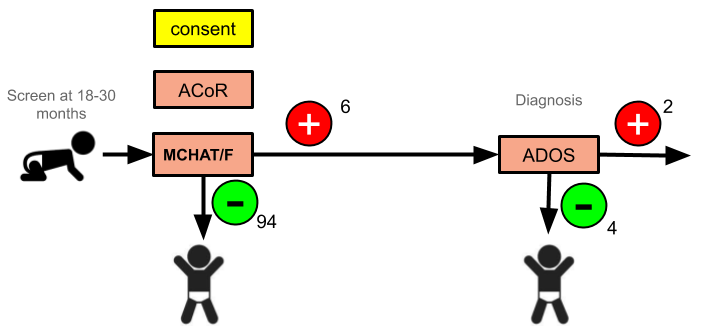
\includegraphics[width=6.25in]{Figures/value}};

%   \end{tikzpicture}
% \end{center}
% \vspace{-10pt}

% \captionN{\textbf{Patient flow logic.} Consenting families with children in appropriate age group (18 to 30 months) are subjected to both M-CHAT/F and \ZERO screens, and a MCHAT-F flag is scheduled for an ADOS evaluation for ascertaining ASD status. Note that by our calculations, for every 100 children, we expect to 6 MCHAT-F flags, out of which 4 on average will get a negative diagnosis by ADOS.}\label{figflow}
% \end{figure}

%  \subsection{Innovation}
% \paragraph*{Paradigm Shift in ASD Screening} Despite extensive documentation of co-morbidities,   a risk estimator that makes reliable predictions for  individuals | based purely on co-morbidity patterns |  has never been reported to the best of our knowledge. The sparsity of available diagnostic codes corresponding to 
% individual subjects, and the general absence of physiological disorders  that would uniquely signal the eventual emergence of symptoms indicative of a clinical ASD diagnosis, combined with the heterogeneity of ASD presentation,  make such an endeavor challenging. In this study we leverage our preliminary work on  the  formulation of a \textit{first-of-its-kind}  framework to make predictions 
% based on models of statistically curated patterns of diagnostic code sequences automatically learned from  sufficiently large databases of electronic health records (EHR), that  achieves an out-of-sample AUC exceeding  $80\%$ for  either gender from just over 2 years of age. The machine learning tools that make this possible are also fundamentally novel, designed to address the specific issues in handling sparse, noisy categorical diagnostic sequences. 
% %\clearpage
% \section{Background Information \& Research Rationale}
% \parskip=8pt
% \setcounter{page}{1}

% \subsection{Significance}
% Autism spectrum disorder is a developmental disability associated with significant social, communication, and behavioral challenges.  The prevalence of ASD  has risen dramatically in the United States from 1 in 10,000 in
%  1972 to 1 in 59 children in 2014, with males  diagnosed at nearly four times the rate of females~\cite{pmid29701730,cdc}.
% There is a current lack of   consensus on whether increased awareness and recent changes in diagnostic practices~\cite{hyman2020identification} can fully explain this  trend~\cite{pmid19737791}. Nevertheless, with   possibly  over 1\% of individuals affected worldwide~\cite{pmid22495912},  ASD is  a human condition with potentially serious negative impacts on individuals, families, and communities. 
% Early detection can and does improve outcomes~\cite{hyman2020identification}, and is of paramount importance when designing interventions, and is aligned with the  envisioned goal of this initiative, as supported by the National Advisory Mental Health Council (NAMHC) (\href{https://www.nimh.nih.gov/funding/grant-writing-and-application-process/concept-clearances/2018/early-screening-for-autism-spectrum.shtml}{https://www.nimh.nih.gov/funding/grant-writing-and-application-process/concept-clearances/2018/early-screening-for-autism-spectrum.shtml}).

% Even though ASD may be reliably diagnosed as early as the  age of two~\cite{cdc},  children frequently remain undiagnosed  until after the fourth birthday~\cite{pmid24529515}. At this time, there are no laboratory tests for ASD, so a careful review of behavioral history and social interactions is necessary for a clinical diagnosis~\cite{volkmar2014practice,hyman2020identification}.  Starting with being flagged by an  initial screen based on standardized checklists presented to parents at the ages between 1.5 and 2 years, a confirmed ASD diagnosis  is a   multi-step process that very often spans  3 months to 1 year. Most of this time is spent waiting to see qualified providers who can carry out the  evaluation necessary for a clinical diagnosis. This extended wait is stressful to families, and  impacts  patient outcomes by  delaying entry into time-critical intervention programs. While   lengthy evaluations~\cite{kalb2012determinants}, cost of care~\cite{bisgaier2011access},  lack of providers~\cite{fenikile2015barriers}, and lack of comfort in diagnosing ASD by primary care providers~\cite{fenikile2015barriers} are all responsible to varying degrees~\cite{gordon2016whittling}, one  obvious factor responsible is the number of false positives produced in the initial ASD-specific screening tools in use today. For example, the  M-CHAT/F, the most widely used screen~\cite{robins2014validation,hyman2020identification},  produces about   over 85 false positives out of every 100 people flagged for further diagnostic evaluation, contributing to extended  queues~\cite{gordon2016whittling}. 
% % @@LATER
% The impact from an excessive number of false positives is exacerbated by the current  limited  access to care and sparse availability of  resources  except near urban academic centers~\cite{gordon2016whittling,althouse2006pediatric}.

% The standardized questionnaires attempt to measure risk by direct observation of behavioral symptoms, as reported by untrained observers (parents). Hence the current screening  tests are only as good as the ability of the questions to discern and disambiguate behavior in infants and toddlers on casual observation, and on the ability of parents and caregivers to correctly interpret and answer the items without bias.
% This has lead to possibility of  under-diagnosis in diverse communities as reflected by the
% lower apparent prevalence among African-American and Hispanic children. Also, children with average or higher-than-average cognitive abilities seem to have been under-diagnosed as reported is large scale population studies~\cite{hyman2020identification}. Borderline cases are typically problematic to screen for due to the possibility  of subjective interpretation that is built into questionnaire based risk assessment. Responses to checklists are clearly confounded by a host of socio-economic (SES) variables, potential interpretive biases, and  cultural differences. The heterogeneity of presentation also causes issues, since a potential plurality of symptom classes makes it harder for clinicians  to recognize borderline cases, or on-the-fly combine observed co-morbidities with scores from  standardized screening tools. 

% In this study, we operationalize a documented aspect of ASD symptomology in  that it has   a wide range  of co-morbidities occurring at much higher rates than in the general population~\cite{hyman2020identification}.
% The \ZERO methodology we propose in this grant can address the aforementioned  complicated  challenges of ASD screening, by distilling incipient predictive patterns of  elevated risk from past medical history of individual  patients, gleaned by machine learning  algorithms from large  de-identified databases of retrospective patient records. Powered by  novel stochastic learning algorithms, we  reverse-engineer sparse noisy uncertain diagnostic code sequences into actionable signatures; in effect giving us  a fundamentally new approach to ASD screening and risk evaluation.

% \paragraph*{Potential  Impact  of  \ZERO In Science and Health}
% An automated   diagnostic or screening capability that might be administered with little or no specialized training, requires no behavioral observations, and is functionally independent of the current tools  has the potential for  immediate transformative  impact on patient care. 

% That such  predictions  of neuropsychiatric  disorders might be possible  from analyzing patterns in individual medical histories   is suggested by the fact  that  parents of children with ASD often notice a diagnosable developmental problem before their child's first birthday; while vision and hearing problems are not uncommon in the first year,  differences in social, communication, and fine motor skills have been reported to be  evident from about 6 months of age~\cite{pmid21410398,herlihy2015parents,chawarska2013decreased}. 

% \section{Study Objectives}

% Specific aims of the study has been enumerated in Section~\ref{secobj}. We outline their significance below.

% \textbf{Significance of Specific Aim 1:} 
% A significant contribution to teh current diagnostic delay arises from families waiting in queue for diagnostic evaluationsr~\cite{gordon2016whittling}. 
% We expect \ZERO to be able to cut down the number of false positives significantly, thus reducing the number of children currently flagged for diagnostic evaluation, which potentially cuts down  the wait-time, thereby reducing diagnostic delays.  Under Specific Aim 1, our goal is to track the fraction of cases where \ZERO correctly signals no-risk while MCHAT-F produces a positive flag.

% \textbf{Significance of Specific Aim 2:} 
% In our preliminary studies, we established that \ZERO outperforms M-CHAT/F by considering the average reported performance of M-CHAT/F in a recent study~\cite{pmid31562252} on a large  cohort with near-universal screening carried out at the Children's Hospital of Philadelphia (CHOP). However, not having observed the \ZERO and the M-CHAT/F scores jointly for individual patients, our preliminary studies lack objective assessment of statistical dependence between the two scores. While the very nature of the methodologies  suggest functional independence, specific Aim 2 will investigate and establish this rigorously. 

% Functional independence from existing tools implies  we can   combine the scores; especially leveraging the population stratification induced by the M-CHAT/F scores as reported by the CHOP study to significantly boost combined screening performance. In particular, since patients in the lower M-CHAT/F score bracket have a smaller chance of an ASD diagnosis compared to the high risk upper brackets, we can tailor the sensitivity/specificity trade-offs in the \ZERO to maximize  either the global PPV or the global sensitivity without losing specificity. Our preliminary results suggest that the expected gains are substantial, with the possibility of doubling the PPV, or increasing the sensitivity by over $50\%$ while keeping the specificity above $95\%$. Specific aim 2 will investigate the e viability of the preliminary results in a pediatric primary care setting.

% \textbf{Significance of Specific Aim 3:} While still lacking the certainty of a diagnostic blood test,  use of subtle patterns emergent in  the diagnostic history to estimate risk might help reduce the subjective component in questionnaire-based screening tools, resulting in reduced effect of potential language and cultural barriers in diverse populations~\cite{hyman2020identification}. With a significant portion of the  cohort expected to be African Americans and Hispanics in our primary care clinic, our comparative investigations will be able to explicitly answer these questions.

% \textbf{Significance of Specific Aim 4:} 
% Despite unprecedented  advances in charting the numerous genetic variations~\cite{Satterstrom484113}, and established to be highly heritable~\cite{sandin17}, the etiology of autism is still unclear~\cite{pmid29691724,pmid29307081}.
% Despite tremendous recent progress, efforts to  identify  causal biomarkers for ASD have had limited success. Currently,  over one hundred genes have been shown to contribute to autism risk~\cite{pmid26402605,pmid25038753,Satterstrom484113}, and it is  estimated that up to 1000 genes might be involved in ASD pathogenesis~\cite{pmid27891212}. Still, genetic interactions and mechanisms have accounted for a limited number of ASD cases~\cite{pmid18414403}, potentially implicating   environmental triggers that  work alongside genetic predispositions. The plausible sources of  risk are estimated to range from prenatal  factors such as maternal infection and inflammation, diet, and  household chemical exposures,  to autoimmune conditions and localized inflammation of the central nervous system after birth~\cite{pmid30971960,pmid30941018,pmid29691724,pmid29307081,pmid27351598,pmid26793298,pmid30095240,pmid25681541}. The heterogeneity of ASD presentation  admits the possibility of a plurality of   etiologies with converging pathophysiological pathways, making the investigation of the etiology of future risk modulation extremely challenging. Specific Aim 4 will aim to unravel clues to mechanistic drivers by charting and categorizing the heterogeneous presentation by the nature of past diagnostic pattern in individual medical histories.

%  \section{Investigational Plan}
 
% \paragraph*{Parallel Screening in Pediatric Primary Clinic} To achieve the specific goals outlined in the specific aims of this study, we will gather data from both the child and the primary caregiver of all patients in the participating UCM primary pediatric primary care clinic, and test the sensitivity and specificity of \ZERO against the most commonly used screening tool M-CHAT/F, by an ADOS-2 based  (near) gold-standard evaluation of   patients flagged by either tool. Using these data and the inferred statistical dependency (or the lack thereof) properties between the screening tools, \ZERO  can tailor the selection of sensitivity/specificity trade-offs  to the particular informant and to the age of the child, with the view to optimizing global characteristics such as maximizing the PPV or the sensitivity of the screening process. Additionally, the \ZERO algorithm will identify categories of heterogeneity that will lead to mechanistic insights into ASD pathobiology.

% Thus, the \ZERO methodology is potentially able to screen instantaneously   every child  in primary care, for whom past medical history is available, with zero administrative and resource burden.
% Our results suggest that \ZERO  has superior predictive performance to existing screening tools, along with a host of other advantages that directly relate to the stated specific aims of this study. 

% The key steps in this project are as  follows (See Fig.~\ref{figflow}):

% \begin{enumerate} 
% [label=$\square$, leftmargin=0pt,
% labelindent=0em, topsep=0.1em, labelsep=*, itemsep=.5em,itemindent=1em]
%  \item 1. Pediatric clinic team  will  adminster  M-CHAT/F to incoming children with 16-30 months.
% \item 2. The University of Chicago Research Informatics Support team will work with the PI and his team to
%   compute the \ZERO score corresponding to individual consenting patients
% \item 3. If flagged by MCHAT-F, the patients will be scheduled for ADOS-2 evaluation (overseen by Dr. Smith). 
% \item 4. The evaluation scores will be analyzed by the PI and his  team to address the specific aims.
% \end{enumerate}

% \subsection*{Cohort Selection} We plan to establish the result as a universal procedure, that is applicable irrespective of population characteristics. Nevertheless, it is clearly conceivable that co-morbidities have demographic dependencies. Unfortunately, the key training dataset (Truven) does not have demographic information. Hence, the \ZERO algorithm at this point does not take such variables into consideration. With a diverse patient population at the University of Chicago, we plan to \textit{not} pre-select population characteristics, but analyze the performance of \ZERO on the different demographic and ethnic groups in the post-processing.

% In this pilot study we plan to have a cohort size of $\approx 200$ children, which should result in nearly 12 MCHAT-F flags, out of which about 8 should be cleared by ADOS. Due to the very small  sample size, we ignore statistical power calculations, but  will analyze if our predicted numbers acceptably match with what we observe in Fig.~\ref{figflow}.
% %
% \subsection*{Risk To Patients} The design of the study guarantees that patients suffer no negative impact from the added \ZERO screen. Indeed, patients who are flagged are to be immediately scheduled for ADOS evaluation which eliminates their wait-times. For some borderline cases, which would have been missed by M-CHAT/F, might get flagged by \ZERO, and be scheduled for ADOS, which they would not have had to do with just M-CHAT/F. But this is a positive outcome. The possibility that \ZERO might have some false positives that are different from that of M-CHAT/F and hence schedule some children for ADOS, who do not have autism is a possibility, and might cause some stress in parents and families. The potential societal benefit gained in lieu of this discomfort is the validation of the expected  performance boost for ASD screening at the population level PPV by up to 100\%.
% %
% \subsection*{Procedures} Eligible patients at the Department of Pediatrics, University of Chicago (patients who present for a well-child visit or any other non-emergency reason) will be asked  for consent for carrying out the \ZERO screen in the background. The algorithm will be already integrated with EPIC, such that indicating this consent on the screen will automatically trigger pulling up the patient medical history if available,  carrying out the calculations, and storing the results to be analyzed in post-processing. If there is a flag either in M-CHAT/F, the attending pediatrician will inform parents of a potential elevated risk of ASD diagnosis, and offer to schedule for an ADOS-2 evaluation.

% All study procedures and consent forms will be approved by the University of Chicago Institutional Review Board.  For all assessments, basic demographic information, recruitment site, medications and diagnoses assigned by the current clinical treatment team, will be obtained from the parent/caregiver and medical record.

% The technical approach of this study consists of the development and extension of the \ZERO methodology from our preliminary studies, and application in a primary care setting with view to carrying out objective comparisons between M-CHAT/F and \ZERO. Furthermore, we plan to assess our ability to boost performance from a conditional combination of the two scores.

% \section{Preliminary Retrospective Results}
% We describe the formulation of the \ZERO score, and the underlying principles that distill the estimated risk from EHR databases.

% We view the task of predicting  ASD diagnoses   as a binary classification problem: sequences of diagnostic codes are classified into positive and control categories, where ``positive'' refers to children eventually diagnosed with ASD, as indicated by the presence of a clinical diagnosis (ICD9 code 299.X) in their medical records. Of the two independent sources of clinical incidence data used in this study,  the primary source used to train our predictive pipeline  is the Truven Health Analytics MarketScan\textsuperscript{\textregistered} Commercial Claims and Encounters Database for the years 2003 to 2012~\cite{hansen2017truven} (referred to  as the Truven dataset). This US national database merges  data contributed by over 150 insurance carriers and large self-insurance companies,  and comprises over  4.6 billion inpatient and outpatient service claims and  almost six billion diagnosis codes. We extracted histories of patients within the age of $0-6$ years, and excluded  patients for whom one or more of the following criteria fails:  1) At least one code pertaining to one of the $17$ disease categories we use (See later for discussion of disease categories) is present in the diagnostic history, 2) The first and last available record for a patient are  at least 15 weeks apart. These exclusion criteria ensure that we are not considering patients who have too few observations. Additionally, during validation runs,  we restricted the control set to patients observable in the databases to those whose last record is not before the first 200 weeks of life. We trained with over  30M diagnostic records (16,649,548 for males and  14,318,303  for females with 9,835 unique  codes).

% While the Truven database is used for both training and out-of-sample cross-validation with held-back  data, our second independent dataset  comprising de-identified diagnostic records for children treated at the University of Chicago Medical Center between the years of 2006 to 2018 (the UCM dataset) aids in further cross-validation. We considered children between the ages of $0-6$ years, and  applied the same exclusion criteria as the Truven dataset. 
% Our datasets are consistent with documented ASD prevalence and median diagnostic age (3 years in the claims database  versus 3 years 10 months to 4 years  in US~\cite{pmid29701730}) with no significant geospatial prevalence variation.

% The significant diversity of diagnostic codes (6,089 distinct ICD-9 codes and 11,522 distinct ICD-10 codes in total in the two datasets), along with the sparsity of codes per sequence and the need to make good predictions as early as possible,  makes this a difficult learning problem, and standard deep learning approaches do not yield sufficiently high predictive performance or statistical power. % (See Supp. Fig.~\ref{SI-EXT-figcompwsoa})
%  Thus, we proceed by  partitioning the  disease spectrum into $17 $ broad categories, $e.g.$ infectious diseases, immunologic disorders, endocrinal disorders etc. Each patient is then represented by $17$ distinct time series, each  tracking an individual disease category. At the population level, these disease-specific sparse stochastic time series are  compressed into specialized Markov models (separately for the control and the treatment cohorts) to identify  the distinctive patterns  pertaining to elevated ASD risk. Each of these inferred models in a Probabilistic Finite State Automaton (PFSA). % See Supplementary Text Section~\ref{SI-sec:PFSA} for details on PFSA inference.  

% We use a novel approach to evaluate subtle deviations in stochastic observations known as the sequence likelihood defect (SLD), to  quantify similarity of observed time-series of diagnostic events to the control vs the \treatment cohorts for individual patients.
% % ###########################################################
% \begin{figure*}[!t]

%   \centering  
   
%   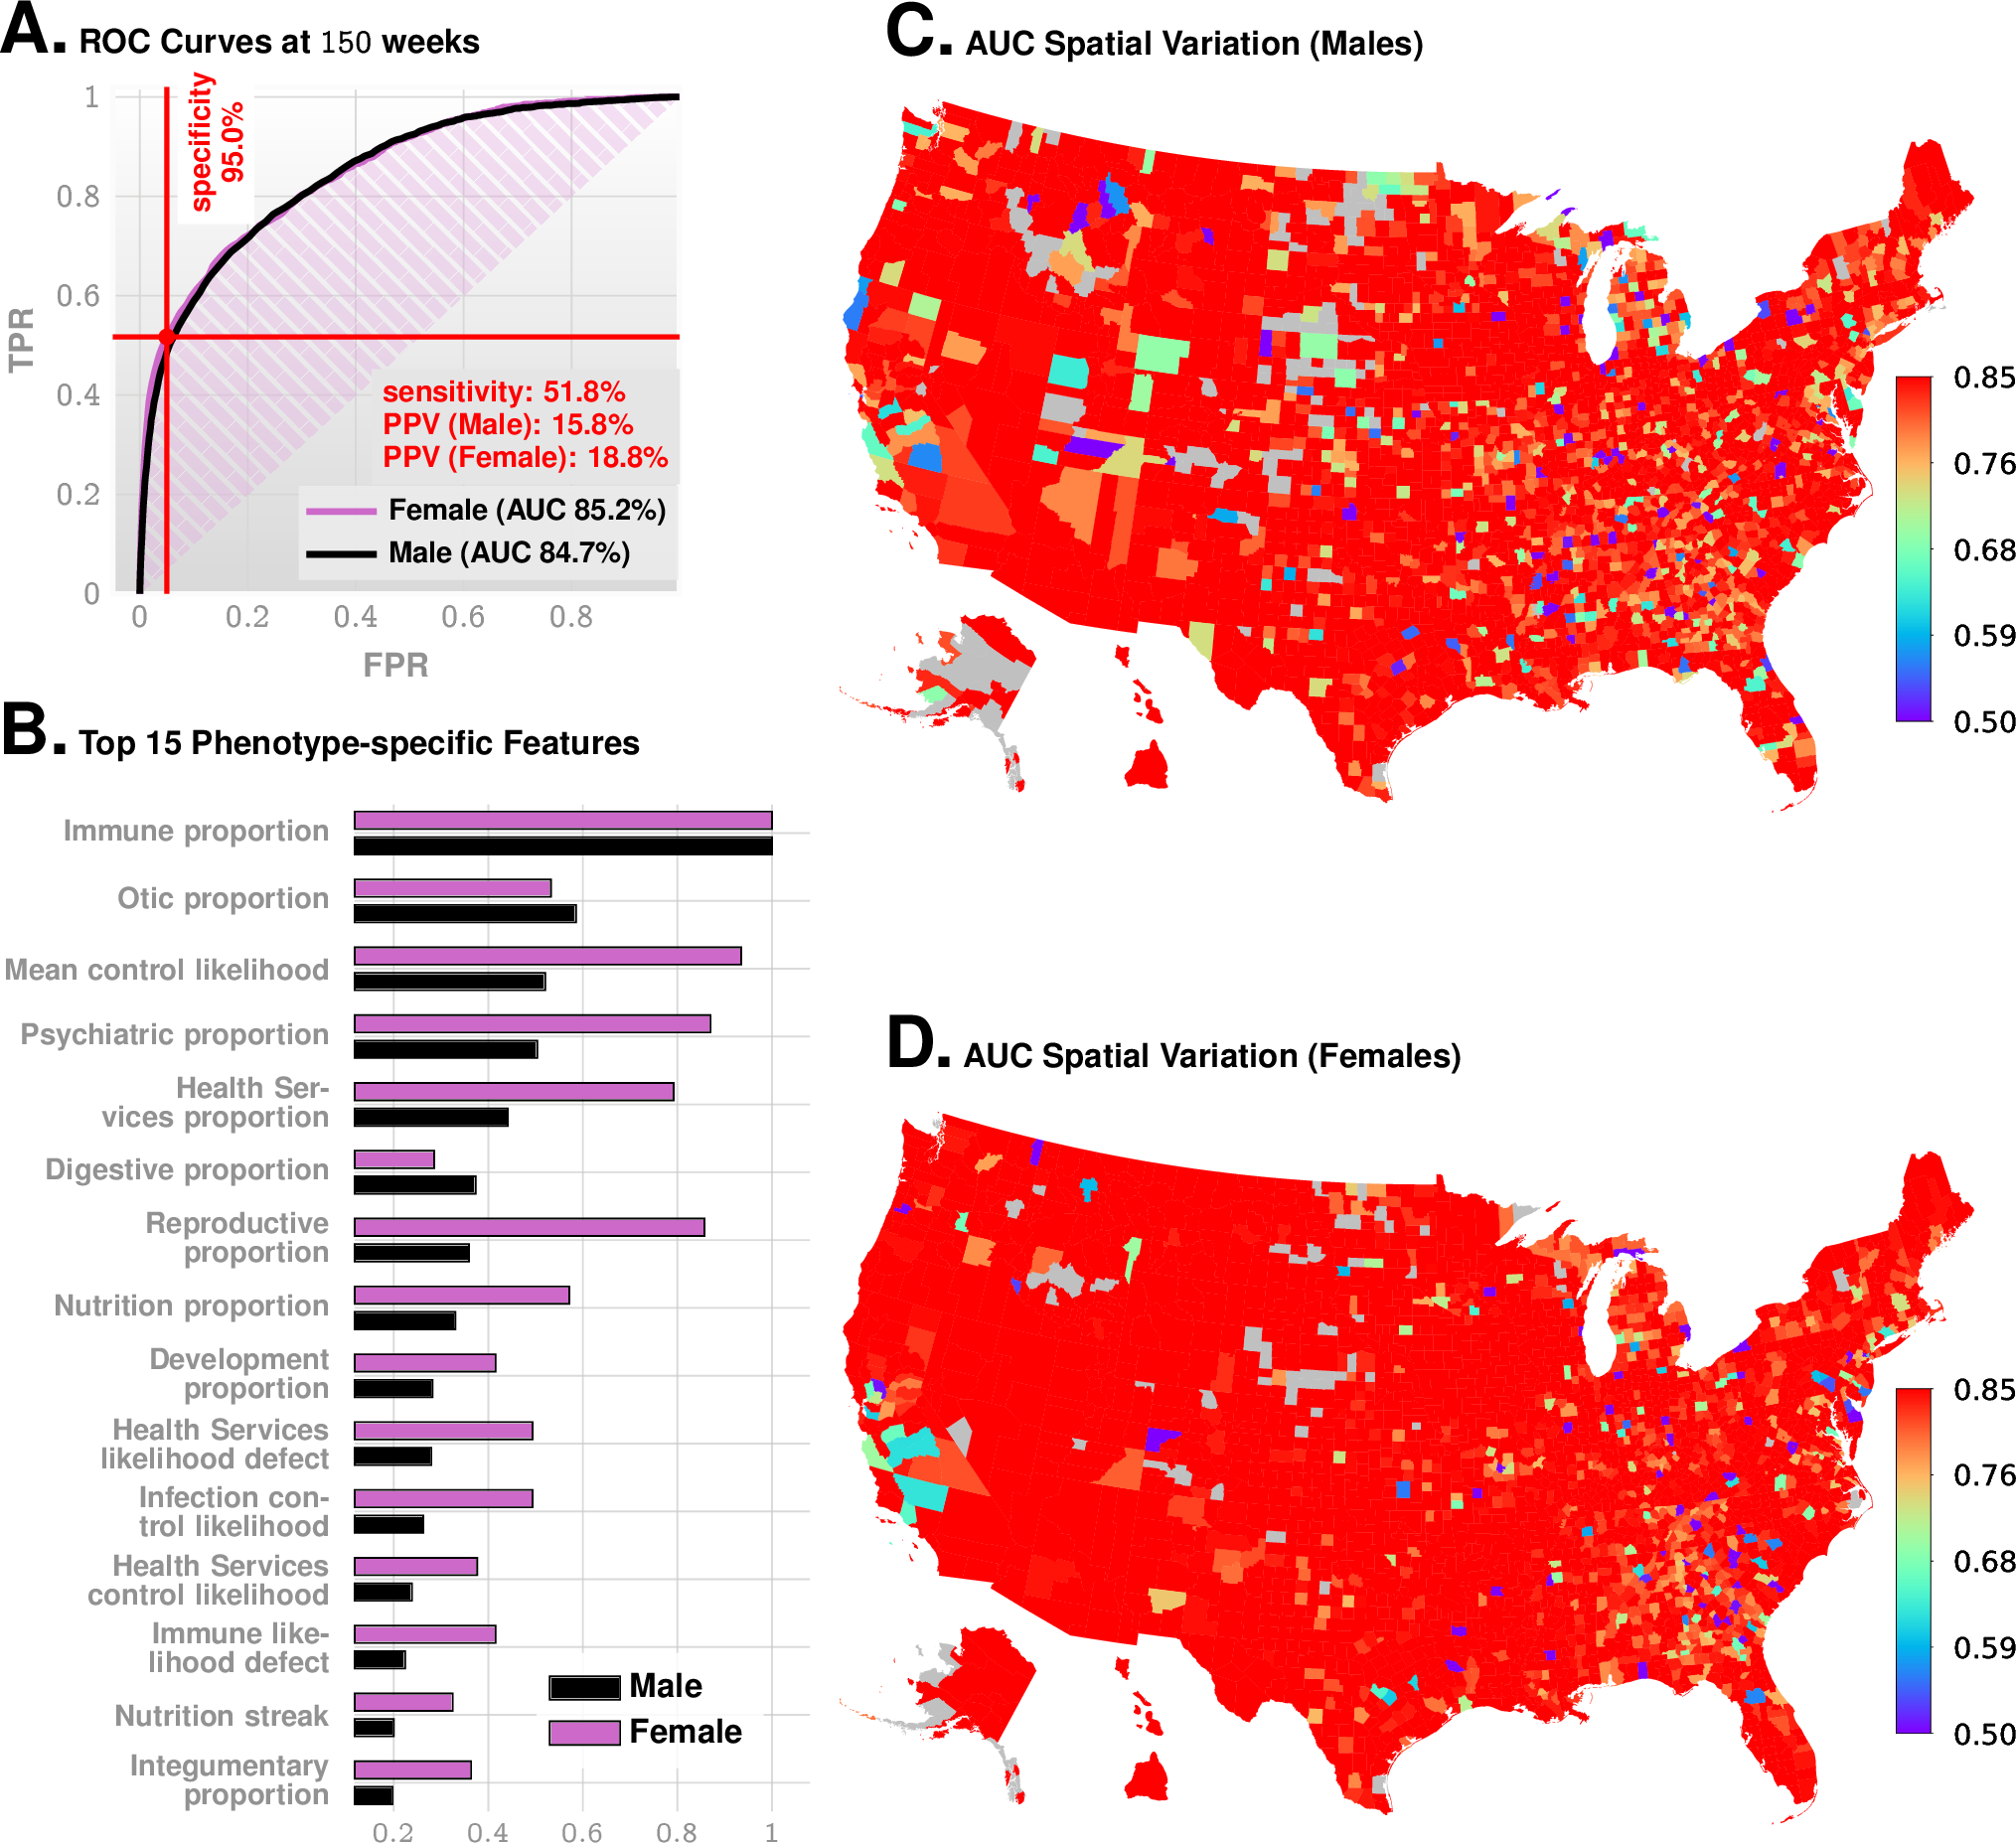
\includegraphics[width=0.85\textwidth]{/home/ishanu/ZED/Research/publications/pub_autism_/Figures/External/perfA.pdf}

%   \captionN{\textbf{Standalone Predictive Performance of \ZERO in Retrospective Studies.} Panel A shows the ROC curves for males and females (Truven data shown, UCM is similar). Panel B shows the feature importance inferred by our prediction pipeline. The most import feature is related to immunologic disorders, and we note that in addition to features related to individual disease categories, we also have the mean control likelihood (rank 3), which may be interpreted as the average likelihood of the diagnostic patterns correspond to the control category as opposed to the \treatment category. Panels C and D show the spatial variation in the achieved predictive performance at 150 weeks, measured by AUC, for males and females, respectively. Gray areas lack data on either positive or negative cases. These county-specific AUC plots show that the performance of the algorithm has  relatively weak geospatial dependence, which is important in the light of current uneven distribution of diagnostic resources. Importantly, not all counties has nonzero number of ASD patients; a high performance in those counties reflects a small number of false positives with zero false negatives.
%   }\label{fig1}
% \end{figure*}
% % ###########################################################
% % \begin{figure}[!ht]
% %  % \vspace{-15pt}
  
% %   \centering 
% %    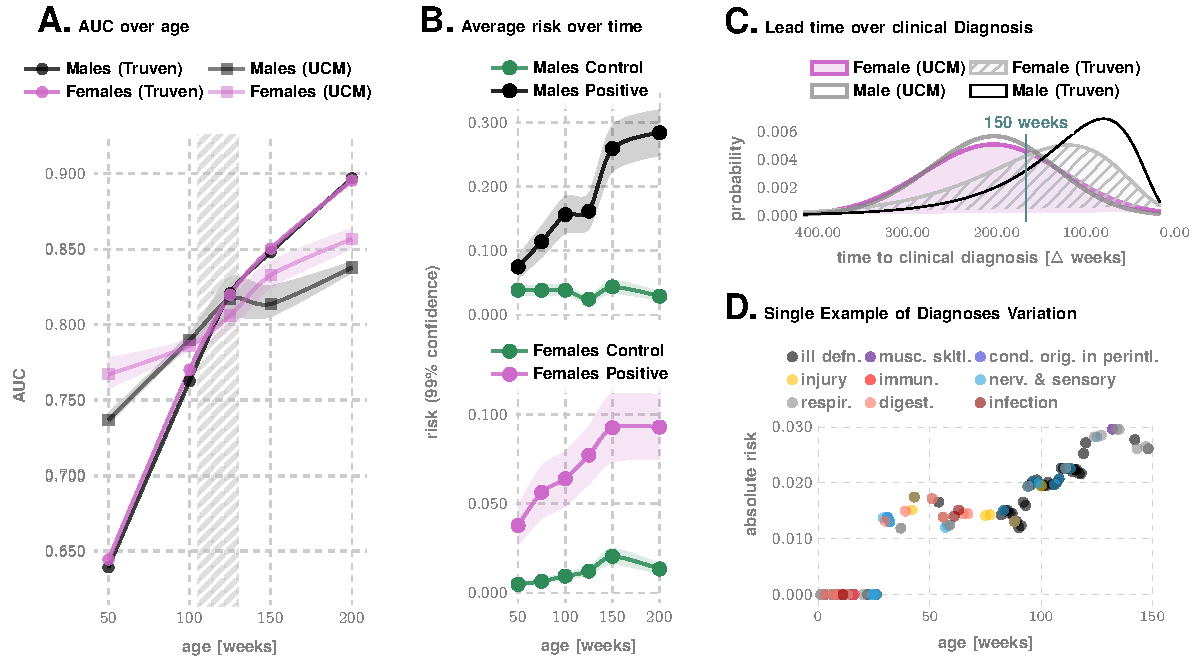
\includegraphics[width=0.9\textwidth]{Figures/test-figure0}
% %    \vspace{-15pt}

% %     \captionN{More details on Predictive Performance and Variation of Inferred Risk. Panel A illustrates AUC achieved as a function of
% %       patient age, for the Truven and UCM datasets. The shaded area outlines the 2 - 2.5  years of age, and  shows that we achieve $>80\%$ AUC for either gender from shortly after 2 years.   Panel B illustrates how the average risk changes with time for the control and the positive cohorts. Panel C shows the distribution of the prediction horizon: the time to a clinical diagnosis after inferred  relative risk crosses $90\%$. Panel d illustrates the risk progression of a specific, ultimately autistic male child in the Truven database. Abbreviations in the legend: ill defn. (Symptoms, Signs, And Ill-Defined Conditions),   musc. skltl. (Diseases Of The Musculoskeletal System And Connective Tissue), cond. orig. in perintl. (Certain Conditions Originating In The Perinatal Period), immun. (Endocrine, Nutritional And Metabolic Diseases, And Immunity Disorders), nerv. \& sensory (Diseases Of The Nervous System And Sense Organs), respir. (Respiratory Disorders), and digest. (Digestive Disorders). %Panel F illustrates  how inferred models differ between the control vs. the \treatment cohorts. On average, models get less complex, implying the exposures get more statistically independent.
% %     }\label{fig2}
% %        \vspace{-15pt}

% % \end{figure}
% %###########################################################
% \begin{figure*}[t]
%   \tikzexternalenable
%   \vspace{-10pt}

%   \centering
  
%   \def\AXISCOL{white}
%   \def\TEXTCOL{gray}
%    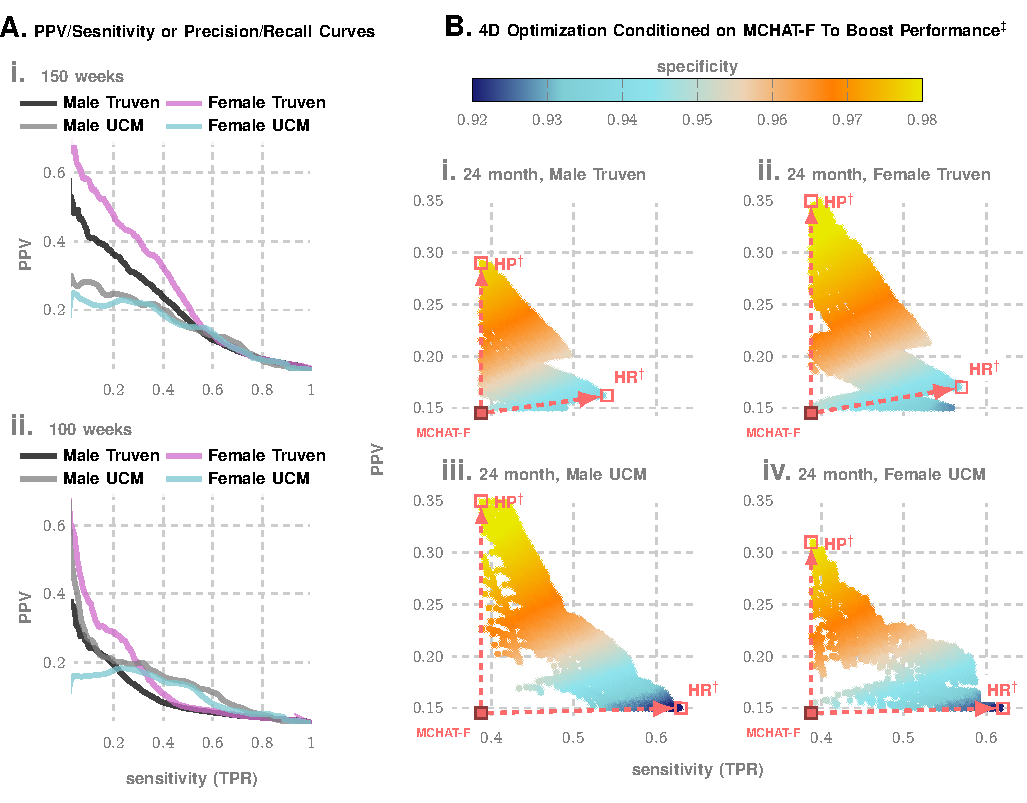
\includegraphics[width=0.8\textwidth]{../results/tex/Figures/External/main2-figure3.pdf}
%  % \vspace{0pt}
%  %  
\pgfplotsset{
    discard if/.style 2 args={
        x filter/.append code={
            \edef\tempa{\thisrow{#1}}
            \edef\tempb{#2}
            \ifx\tempa\tempb
                \def\pgfmathresult{inf}
            \fi
        }
    },
    discard if not/.style 2 args={
        x filter/.append code={
            \edef\tempa{\thisrow{#1}}
            \edef\tempb{#2}
            \ifx\tempa\tempb
            \else
                \def\pgfmathresult{inf}
            \fi
        }
    }
  }

  \begin{tikzpicture}[font=\bf\sffamily\fontsize{8}{10}\selectfont]
  \def\TEXTCOL{gray}

  \def\DATAPATH{../../revision_results/roc/restricted_neg_len/RAW/}
  \def\datafile{\DATAPATH/thisRFall.csv}


  \def\AXISCOL{white}
  \def\WDTa{1.85in}
  \def\HGTa{2in}
  \def\HGT{1.2in}
  \def\WDT{1.2in}
  \def\MXCOLB{gray}
  \def\FXCOLB{CadetBlue3}
  \def\OPC{.75}
  \def\OPCB{.65}
  \def\LWDT{0.7mm}
  \def\SKIP{4}  
  \def\WDTa{1.75in}
  \def\WDTb{1.25in}
  \def\HGTa{1.65in}
  \def\SKIP{5}
  \def\SKIPB{1}
  \def\LCOL{black}

  \node[] (A0) at (0,0) {};
  \node[anchor=center] (N) at (A0.south)
  {
    \begin{tikzpicture}[text=\TEXTCOL, ]
      \begin{groupplot}
        [name=Agg,
        group style={
          group name=Ag,
          group size=3 by 1,
          xlabels at=edge bottom,
          xticklabels at=edge bottom,
          vertical sep=.75in,
          horizontal sep=.8in,
        },        ,legend cell align={left},
        legend style={anchor=east,at={(-0.12,1.1)},
          inner sep=3pt,
          draw=none,
          fill=white,fill opacity=.850,
          align=left,anchor=west,
          text opacity=1,
          font=\bf\sffamily\fontsize{8}{9}\selectfont,text=black},legend columns=2, 
        name=K,
        clip=true,,
        width=\WDTa,
        height=\HGTa,
        scale only axis=true,
        enlargelimits=false,
        axis on top=false,
        % axis background/.style={
        %   shade,top color=transparent!5,bottom color=transparent!5},
        axis line style={\AXISCOL, opacity=1,ultra  thick, 
          rounded corners=0pt}, 
        grid,
        grid style={thick,dashed, gray!40},
        % xticklabel style={xshift=0.05in,yshift=-.05in},
        xlabel style={yshift=.05in,text=\TEXTCOL},
        ylabel style={align=center,,text=\TEXTCOL,anchor=center,
          yshift=-.15in},
        % tickpos=left,
        ytick align=outside,
        xtick align=outside,
        major tick length=0pt,
        scaled y ticks = false,
        y tick label style={/pgf/number format/fixed,
          /pgf/number format/1000 sep = \thinspace % Optional if you00 separator 
        },
        ylabel={PPV},xlabel={sensitivity (TPR)},point meta=explicit,
        colorbar style={width=.1in,y tick label style={/pgf/number format/fixed,/pgf/number format/precision=2,/pgf/number format/fixed zerofill,
     /pgf/number format/1000 sep = %\thinspace % Optional if you want to replace comma as the 1000 separator 
      },}
        % extra x ticks={1},extra x tick labels={1}
        ]

   \nextgroupplot[colorbar horizontal,xmin=.98,extra x ticks={1},colorbar style={at={(0,1.2)},title={prevalence},title style={yshift=-.1in},
          height=.1in,scaled x ticks=false,
x tick label style={/pgf/number format/fixed,
          /pgf/number format/precision=3,/pgf/number format/fixed zerofill,
          /pgf/number format/1000 sep = %\thinspace % Optional to replace comma as the 1000 separator 
        },
          xticklabel style={yshift=-.025in},},ylabel={MCHAT-F relative wait time},xlabel={MCHAT-F relative sensitivity}]
        \pgfplotsset{
colormap={hot}{color(0cm)=(lightgray!70); color(1cm)=(lightgray!80); color(2cm)=(lightgray!80!Bisque1); color(3cm)=(Bisque1!90!Tomato); color(4cm)=(Tomato); color(5cm)=(Red1)}
}
\addplot [mesh, each nth point=\SKIP, filter discard warning=false, 
        unbounded coords=discard,line width=\LWDT]table [col sep=comma,x=rs,y=tm,meta=rho,
discard if not={gender}{M},
restrict expr to domain={\thisrow{c}}{0.95:1},
restrict expr to domain={\thisrow{rho}}{0.017:0.024},
restrict expr to domain={\thisrow{rs}}{1:1.5},
] {\datafile};   

\node[anchor=west] (x11) at (axis cs:1,0.7) {};
\node[anchor=west] (x12) at (axis cs:1.35,0.525) {};
\node[anchor=west] (xx) at (axis cs:1,0.5) {};


        \nextgroupplot[colorbar,width=\WDTb,xshift=-.2in, title={{\Large i.}  specificity shown by color},colorbar style={xshift=-.1in,,ylabel=specificity,ylabel style={yshift=-.2in}},title style={yshift=.12in,xshift=.15in}]
        \pgfplotsset{
colormap={hot}{color(0cm)=(MidnightBlue); color(1cm)=(CadetBlue2!90!black); color(2cm)=(CadetBlue1!93!black); color(3cm)=(Bisque1!93!black); color(4cm)=(DarkOrange1); color(5cm)=(Yellow2!93!black)}
}

\addplot [mesh, very thick, , each nth point=\SKIPB, filter discard warning=false, 
        unbounded coords=discard
%point meta min=0.92, point meta max=0.98
]table [col sep=comma,x=s,y=p,meta=c,
%discard if not={gender}{M},
restrict expr to domain={\thisrow{c}}{0.966:1},restrict expr to domain={\thisrow{rho}}{0.012:1}] {\datafile};
\node[anchor=west] (x01) at (axis cs:0.5,0.35) {};
\node[anchor=west] (x02) at (axis cs:0.25,0.25) {};

        \nextgroupplot[colorbar,ylabel={},width=\WDTb, title={{\Large ii.}   prevalence shown by color},colorbar style={y tick label style={/pgf/number format/fixed,/pgf/number format/precision=3,/pgf/number format/fixed zerofill,
     /pgf/number format/1000 sep = %\thinspace % Optional if you want to replace comma as the 1000 separator 
      },xshift=-.1in,,ylabel=prevalence,ylabel style={yshift=-.2in}},title style={yshift=.12in,xshift=.15in}]
        \pgfplotsset{
colormap={hot}{color(0cm)=(lightgray!70); color(1cm)=(lightgray!80); color(2cm)=(lightgray!80!Bisque1); color(3cm)=(Bisque1!90!Tomato); color(4cm)=(Tomato); color(5cm)=(Red1)}
}
\addplot [mesh, very thick, each nth point=\SKIPB, filter discard warning=false, 
        unbounded coords=discard]table [col sep=comma,x=s,y=p,meta=rho,
%discard if not={gender}{M},
restrict expr to domain={\thisrow{c}}{0.966:1},restrict expr to domain={\thisrow{rho}}{0.012:1}] {\datafile};

\node[anchor=west] (x1) at (axis cs:0.5,0.35) {};
\node[anchor=west] (x2) at (axis cs:0.25,0.25) {};

      \end{groupplot}
\node[anchor=west, fill=white] (x1) at (x1) {Female};
\node[anchor=center, fill=white] (x2) at (x2) {Male};
\draw[-{Latex},thick,\MXCOL] (x2) -- ($(x2)!.3!(x1)$);
\draw[-{Latex},thick,\FXCOL] (x1) -- ($(x1)!.4!(x2)$);


\node[anchor=west, fill=white] (x01) at (x01) {Female};
\node[anchor=center, fill=white] (x02) at (x02) {Male};
\draw[-{Latex},thick,\MXCOL] (x02) -- ($(x02)!.3!(x01)$);
\draw[-{Latex},thick,\FXCOL] (x01) -- ($(x01)!.4!(x02)$);

\node[anchor=west, fill=white,text=IndianRed1] (x11) at (x11) {CHOP{\color{\TEXTCOL}$^\bigstar$}};
\node[anchor=center, fill=white] (x12) at (x12) {CDC{\color{\TEXTCOL}$^\bigstar$}};
\draw[-{Latex},thick,] (x12) -- ($(x12)!.3!(x11)$);
\draw[-{Latex},thick] (x11) -- ($(x11)!.35!(x12)$);

\draw[-{Latex},very thick,\LCOL]  ($(xx)!1.2in!(xx.north)$) --(xx) node [pos=0,above,right,fill=white,align=center,text=\LCOL,yshift=.1in] {wait-time\\cut in half};

\end{tikzpicture}
  }; 
 \node[anchor=south west] (L1) at ([yshift=-.05in]N.north west) {{\Large C.} Wait time  vs  Recall   (specificity$>97\%$)};
 \node[anchor=south west] (L2) at ([xshift=.4in]L1.south east) {{\Large D.} Pareto fronts for 4D operating point choices wrt prevalence variations};

\node[anchor=north west,align=left,font=\sffamily\fontsize{7}{7}\selectfont] (L3) at (N.south west) {$\ddag$Using population statsitics from CHOP study (See SI-Table~\ref{SI-tabCHOP}). $^\dag$HP: High precision/PPV operating point, HR: High recall/sesitivity operating point \\{\color{\TEXTCOL}$^\bigstar$}CHOP estimates prevalence in its study to be $2.23\%$, while CDC estimates are lower at $1.7\%$};

\end{tikzpicture}

 

%  \vspace{-10pt}

%  \captionN{\textbf{Metrics relevant to clinical practice: PPV vs Sensitivity trade-offs.} Panel A shows the precision/recall curves, $i.e.$,  the trade-off between PPV and sensitivity. Panel B shows how we can boost performance using population stratification from the distribution of M-CHAT/F scores in the population, as reported by the CHOP study~\cite{pmid31562252}. Panel C illustrates the boosted performance compared to M-CHAT/F alone,
%    mesured by the relative percentage increase in sensitivity, and percentage decrease in postive screens. Note that the population prevalence impacts this optimization, and hence  we have  a distinct  curve for each prevalence value ($1.7\%$ is the CDC estimate, while $2.23\%$ is reported by the CHOP study).  The two extreme operating zones marked as High Precision (HP) and High Recall (HR): if we choose to operate in HR, then we do not reduce the number of positive screens by much, but maximize sensitivity, while by operating in HP, we do not increase seinsitivity by much but double the PPV achieved in current practice. Note in all these zones we maintain specificity above $95\%$, which is the current state of art, implying that by doubling the PPV, we can halve the number of positive screens currently reported, thus potentially sharply reducing the queues and wait-times. }\label{figprc}
% \end{figure*}
% % ###########################################################

% % While the Truven database is used for both training and out-of-sample cross-validation with held-back patient data, our second independent dataset (referred to as the UCM dataset) consisting of de-identified diagnostic records for children treated at the University of Chicago Medical Center between the years of 2006 to 2018, aids in further cross-validation. We considered children between the ages of $0-5$ years, and  applied the same exclusion criteria as the Truven dataset.

% % \subsection*{Time-series Modeling of  Diagnostic History}
% % Individual diagnostic histories  can have long-term memory~\cite{ltgranger80}, implying that the order, frequency, and comorbid interactions between diseases are potentially  important for assessing the future risk of our target phenotype. 
% % Our  approach to analyzing patient-specific  diagnostic code sequences consists of representing the medical history of each patient as a set of stochastic categorical time-series | one each for a specific group of related disorders |  followed by the inference of stochastic generators  for  these individual data streams. These inferred generators are from a special class of  Hidden Markov Models (HMMs), referred to as Probabilistic Finite State Automata (PFSA)~\cite{CL12g}. The inference algorithm we use is distinct from classical HMM learning, and has important advantages related to the ability to infer structure, and sample complexity. We infer a separate class of models for the \treatment and control cohorts, and then the problem reduces to determining the probability that the short diagnostic history from a  new  patient arises from the \treatment as opposed to the control category of the inferred models. Importantly,  the individual histories are typically short, often have large randomly varying  gaps, and we have no guarantee that model-structural assumptions~\cite{Stoyanov2010,Shumway2000} (linearity, additive noise structure, etc.)  often used in the standard time-series analysis is applicable here. Also, the categorical observations are drawn  from a large alphabet of possible  diagnostic codes, which degrades  statistical power. 

% % \subsection*{Step 1: Partitioning The Human Disease Spectrum} To address these issues, we begin by partitioning the human disease spectrum into  $17$ non-overlapping  categories, which remain fixed throughout the analysis. Each category is defined by a set of diagnostic codes from the International Classification of Diseases, Ninth Revision (ICD9).
% % For this study, we considered $9,835$ distinct ICD9 codes (and their ICD10 General Equivalence Mappings (GEMS)~\cite{GEMS} equivalents). We came across 6,089 distinct ICD-9 codes and 11,522 distinct ICD-10 codes in total in the two datasets we analyzed. Transforming the diagnostic histories to report only the broad categories   reduces the number of distinct codes that the pipeline needs to handle, thus improving statistical  power.  The trade-offs for this increased power consist of 1) the loss of distinction between disorders in the same category, and  2) some inherent subjectivity in determining the constituent ICD9 codes that define each category, $e.g.$ an ear infection may be classified either an otic disease or an infectious one.


% % We do not pre-select the phenotypes; we want our algorithm to seek out the important patterns without any manual curation of the input data. The limitation of the set of phenotypes to $9835$ unique codes arises from excluding patients from the database who have very few and rare codes that will skew the statistical estimates. Next, we process raw diagnostic histories to generate data streams that report only the categories instead of the exact codes. For each patient, his or her  past  medical history is a sequence $(t_1,x_1),\cdots,(t_m,x_m)$, where $t_i$ are timestamps and $x_i$ are ICD9 codes diagnosed at time $t_i$.  We map individual patient history to a three-alphabet  time series $z^k$ corresponding to the disease category $k$,  as follows. For each week $i$,
% % \cgather{\label{eq1}
% %   z^k_i =  \left \{ \begin{array}{ll}
% %                        0 & \textrm{if no diagnosis codes  in week } i\\
% %                        1 & \textrm{if there exists a diagnosis of category $k$ in week } i\\
% %                        2 & \textrm{otherwise}
% %                       \end{array} \right.
% %                   }The time-series $z^k$ is terminated at a particular week if the patient is diagnosed with ASD the week after. 
% % In summary, each patient is now represented by $17$ mapped trinary series, which we  use next  to infer population-level PFSA models. 

     

% % \subsection*{Step 2: Model Inference \& The Sequence Likelihood Defect}
% % The mapped series, stratified by  gender, disease-category, and ASD diagnosis-status are considered to be independent realizations or sample paths from  relatively invariant stochastic dynamical systems; and we explicitly model these systems as HMMs. We model the \treatment and the control cohorts for each gender, and in  each disease category separately, ending up with a total of $68$ HMMs at the population level ($17$ categories, $2$ genders, $2$ cohort-types: \treatment and control). Each of these inferred models is  a PFSA;  a directed graph with probability-weighted edges, and acts as an optimal generator of the  stochastic process driving the  sequential appearance of the three letters (as defined by Eq.~\eqref{eq1})  corresponding to each gender, disease category, and cohort-type. % These models  are very nearly assumption-free beyond the requirement that  the processes be statistically stationary or slowly varying.  In particular, these models are not  \textit{a priori}  constrained by any structural motifs, complexity, or size, and are   compact representations of  patterns emerging in the mapped time series. Additionally, when learning models for sets of diagnostic histories corresponding to a patient cohort, the histories can be of different lengths.
% % The modeling objective here is to exploit the relative differences in these  probabilistic  models to reliably infer the cohort-type of a new patient from their  individual sequence  of past diagnostic codes.
% % %
% % To that effect, we generalized the well-known notion of Kullbeck-Leibler (KL) divergence~\cite{Cover,kullback1951} between probability distributions to a divergence $\mathcal{D}_{\textrm{KL}}(G \vert \vert H)$ between ergodic stationary categorical stochastic processes~\cite{doob1953stochastic} $G,H$ as:
% % \cgather{
% %   \mathcal{D}_{\textrm{KL}}(G \vert \vert H) = \lim_{n\rightarrow \infty} \frac{1}{n}  \sum_{x:|x| = n}p_G(x)\log\frac{p_G(x)}{p_H(x)}  }\noindent
% % where $\vert x\vert $ is the sequence length, and $p_G(x) ,p_H(x) $ are the probabilities of sequence $x$ being generated by the processes $G,H$ respectively.
% % Defining the  log-likelihood of  $x$ being generated by a process $G$ as :
% % \cgather{
% %     L(x,G)= -\frac{1}{\vert x\vert}\log p_G(x) 
% %   }\noindent
% %   The cohort-type for an observed sequence $x$ | which is actually generated by the hidden process $G$ | can be formally inferred from observations based on the following provable relationships:
% %   \begin{subequations}\label{eqR}\cgather{
% %     \lim_{\vert x \vert \rightarrow \infty}L(x,G) = \mathcal{H}(G)   \\
% %     \lim_{\vert x \vert \rightarrow \infty } L(x,H)  =\mathcal{H}(G) +  \mathcal{D}_{\textrm{KL}}(G \vert \vert H)   
% %     }\end{subequations} where  $\mathcal{H}(\cdot)$ is the entropy rate of a process~\cite{Cover}. Importantly, Eq.~\eqref{eqR} shows that the computed likelihood has an additional non-negative contribution from the divergence term, when we choose the incorrect generative process.  Thus, if a  patient is eventually going to be diagnosed with ASD, then we expect that the disease-specific mapped series corresponding to  her diagnostic history be modeled by the PFSA in the \treatment cohort. Denoting the PFSA corresponding to disease category $j$ for \treatment and control cohorts as $G^{j}_+,G^{j}_0$ respectively, we can compute the \textit{sequence likelihood defect} (SLD, $\Delta^j$) as:
% %     \cgather{
% %       \Delta^j \triangleq L(G^{j}_0,x) - L(G^{j}_+,x) \rightarrow \mathcal{D}_{\textrm{KL}}(G^{j}_0 \vert \vert G^{j}_+) \label{eq6}
% %       }With  the inferred population-level PFSA  models and  the individual diagnostic history, we can now estimate the SLD measure on the  right-hand side of Eqn.~\eqref{eq6}. The higher this likelihood defect, the higher  the similarity of the patient's history  to ones that have an eventual ASD diagnosis with respect to the disease category being considered. SLD is the core novel analytic tool used in this study  to tease out  information relevant to the risk estimator and is key to the design of our risk estimation pipeline.

% % \subsection*{Step 3: Risk Estimation Pipeline With Semi-supervised \& Supervised Learning Modules}
% % Ultimately, the risk estimation pipeline operates on patient specific information limited to the
% % gender and available  diagnostic history from birth, and produces an estimate of the relative risk of ASD diagnosis at a specific age, with an associated  confidence value.
% % To learn the parameters and associated model structures of  this pipeline, we transform the patient specific data to a set of engineered features, and the feature vectors realized on the
% % \treatment and control sets are then used to train a gradient-boosting classifier~\cite{gbm02}. Of the set of engineered features, the most important are the  disease-category-specific SLD described above. For example, if $SLD > 0$ for a specific patient for every disease category, then he or she is likely to have an ASD diagnosis eventually. However, not all disease categories are equally important for this decision; parametric  tuning of the classifier allows us to infer the optimal combination weights, as well as compute the relative risk  with associated confidence. In addition to category-specific SLDs, we use a range of other derived quantities as features, including the mean and variance of the defects computed over all disease categories, the occurrence frequency of the different disease groups, etc. 
% % The top $15$ features used in our pipeline may be ranked in order of their relative importance (See Fig.~\ref{fig1}B), by estimating the loss in performance when dropped out of the analysis, and the importance of  infections and immunologic disorders are clearly evident (See Fig.~\ref{fig1}B).  

% % % PFSA : TRAIN : TEST ratio ::: [.2, .256, .544]
% % % [*M*]
% % % Total size : 2.94M
% % % Set sizes: 590k, 750k, 1.6M
% % % [*F*]
% % % Total size : 2.75M
% % % Set sizes: 550k, 700k, 1.5M
% % %\subsection*{Receiver Operating Characteristic \& Relative Risk Calculation}
% \subsection*{Calculating Relative Risk}
% Our pipeline maps medical histories to a  score, which is interpreted as a raw indicator of 
% risk | higher this value, higher the probability of a future diagnosis. However, to make crisp predictions, we must choose  a decision threshold for this raw score. Conceptually identical to the notion of Type 1 and Type 2 errors in classical statistical analyses, the choice of a threshold trades off false positives (Type 1 error) for false negatives (Type 2 error): choosing a small threshold  results in predicting a larger fraction of future diagnoses correctly, $i.e.$ have a high true positive rate (TPR), while simultaneously suffering from a higher false positive rate (FPR), and vice versa.
% We choose thresholds for the standalone \ZERO method by  maximizing the $F_1$-score, defined as the harmonic mean of sensitivity and specificity, to make a   balanced trade-off between the two kinds of errors.
% %
% The \textit{relative risk} is then defined as the ratio of the raw pipeline score to the chosen decision threshold. While the raw score does not give us  actionable information,  the relative risk being close to or greater than 1.0 for a specific child signals the need for intervention.
% %
% \subsection*{Standalone Predictive Performance}
% % %####################################
% \def\RCOL{\rowcolor{teal!40}}
% %#################################### 
% \begin{table}[t]   
% \centering 
% \captionN{Standalone \ZERO PPV Achieved}\label{tabssp}
% \footnotesize
% \mnp{\textwidth}{%\vskip .1em
% \vspace{-15pt}

% \scriptsize (For Comparison M-CHAT/F Performance:  sensitivity=$38.8\%$, specificity=$95\%$, PPV=$14.6\%$ between within 26 months ($\approx$112 weeks))\\
% \vskip .1em}
% %
% %
% \begin{tabular}{L{.75in}|L{.75in}|L{.75in}|L{.5in}|L{.5in}|L{.75in}}
% \hline
% week&spec.&sens.&PPV&sex&dataset\\\hline
100&0.92&0.39&0.14&F&UCM\\\hline
100&0.95&0.39&0.19&M&UCM\\\hline
100&0.93&0.39&0.13&F&Truven\\\hline
100&0.91&0.39&0.10&M&Truven\\\hline
%\RCOL 112&0.94&0.35&0.17&F&UCM\\\hline
\RCOL 112&0.93&0.39&0.16&F&UCM\\\hline
\RCOL 112&0.95&0.39&0.20&M&UCM\\\hline
\RCOL 112&0.96&0.39&0.22&F&Truven\\\hline
\RCOL 112&0.95&0.39&0.17&M&Truven\\\hline
% 150&0.94&0.39&0.19&F&UCM\\\hline
% 150&0.98&0.39&0.34&F&Truven\\\hline
% 150&0.97&0.39&0.26&M&Truven\\\hline
% 150&0.97&0.39&0.26&M&UCM\\\hline

% \end{tabular}
% \end{table}  
% %####################################
% % %####################################
% The standalone performance of our risk estimator is summarized  in Fig.~\ref{fig1}A. The task of predicting if a patient has a future ASD diagnosis, at an earlier date compared to the clinical diagnosis,  may be viewed as a binary classification problem.
% In our case, we achieve an out-of-sample AUC of $82.3\%$ for males and $82.5\%$ for females at $125$ weeks of age for the Truven dataset. In the UCM dataset, our performance is comparable: $83.1\%$ and $81.3\%$ for males and females respectively at $125$ weeks of age. The good agreement of the out-of-sample performance on these independent datasets lends strong evidence for the claims made in this study. The specificity, sensitivity, PPV trade-offs are shown in Table~\ref{tabssp}.


% We enumerate the top $15$ predictive features in Fig.~\ref{fig1}B. 
% We also computed the county-specific performance of the risk pipeline for the Truven dataset, and we got nearly uniform performance across the country for both genders, with the exception of  few isolated counties lacking patients in the appropriate age groups (See Fig.~\ref{fig1}, panels C and D) which prevented us from estimating AUC for those counties. Thus the performance of the algorithm is relatively agnostic to the number of local diagnoses, which is import in light of the fact that   crucial diagnostic resources currently have a very uneven distribution (only 7\% of developmental pediatricians practice in rural areas, and some states in US do not even have a developmental pediatrician~\cite{gordon2016whittling,althouse2006pediatric}).


% \subsection*{Calculating PPV, Sensitivity \& Specificity Trade-offs \& M-CHAT/F Comparison}
% The sensitivity vs PPV plots, also known as the precision-recall curves (See Fig.~\ref{figprc}A) are constructed in a similar fashion as the ROC curves by varying the decision threshold. These curves  allow direct comparison with the  state of the art screening tests,$e.g.$, M-CHAT/F, in a manner that is most relevant to clinical practitioners.
% %
% Guthrie $\etal$~\cite{pmid31562252} from Children's Hospital of Philadelphia (CHOP) has recently demonstrated that when applied as a nearly universal screening tool, M-CHAT/F has a sensitivity of 38.8\%, specificity of 94.9\% and PPV of 14.6\%, implying that out of every 100 children who in fact ave ASD, the M-CHAT/F flags about 39, and out of every 100 children it flags, about 85 are false positives. The PPV is affected by the prevalence of the disease. This work is the only large-scale study of M-CHAT/F (n=20,375) we are aware of with sufficient follow-up after the age of four years to provide a reasonable degree of confidence in the reported performance values.

% Comparing the performance metrics achieved at different age groups across data sets and genders for our pipeline (See Table~\ref{tabssp}), we conclude that our approach produces a strictly superior PPV (exceeding M-CHAT/F PPV by at  $14\%$ (14.1-33.6\%) when sensitivity and specificity are held at comparable values around the age of 26 months ($\approx 112$ weeks). We cannot compare at other operating points due to limited availability of M-CHAT/F performance characterization at other time points.
% %###############################################
% \begin{table}[t]
%   \centering

%   \captionN{Population Stratification Results on large M-CHAT/F Study(n=20,375)  reproduced from Guthrie $\etal$~\cite{pmid31562252} }\label{tabCHOP}
% \footnotesize
%   \begin{tabular}{C{.65in} | L{1.5in}|L{1.5in}|L{1in}|L{1in}||L{.55in}}\hline
%  \bf \sffamily   Id &  \bf \sffamily Sub-population & \bf \sffamily Test Result & \bf \sffamily ASD pos. & \bf \sffamily ASD Neg. & \bf \sffamily Total \% \\\hline
%    A &  M-CHAT/F $\geqq 8$ & Positive & 0.34\% & 0.64\% & 0.99\% \\\hline
%   B &   M-CHAT/F $\in [3,7]$ & Positive (follow-up)& 0.52\% & 4.39\% & 4.91\% \\\hline
%  C &    M-CHAT/F $\in [3,7]$ & Negative (follow-up)& 0.14\% & 3.1\% & 3.24\% \\\hline
%   D &   M-CHAT/F $\in [0,2] $ & Negative & 1.22\% & 89.63\% & 90.86\% \\\hline\hline
%     Total \%& &   &2.23\% & 97.77\% & 100\% \\\hline
%     \end{tabular}
% \end{table}
% %###############################################
% \subsection*{Boosting Performance Via Leveraging Population Stratification Induced By M-CHAT/F}
% In our retrospective study, we leveraged the population stratification induced by an existing independent screening test (MCHAT-F) to improve combined performance. Here a combination  refers to the conditional choice of the sensitivity/specificity trade-offs for our tool in each sub-population such that the overall performance is optimized with respect to whether we wish to maximize the PPV or the sensitivity at a specified minimum level of specificity. Assume that there are $m$ sub-populations such that:
% the sensitivities, specificities achieved, and the prevalences in each sub-population are given by $s_i,c_i$ and $\rho_i$ respectively, with $ i \in \{1,\cdots, m\}$. Let $\beta_i$ be the relative size of each sub-population. Then, we can show:
% \begin{subequations}\label{eqscpop}
% \cgather{
%   s= \sum_{i=1}^m s_i \gamma_i  , \textrm{ and } 
%   c= \sum_{i=1}^m c_i \gamma_i' %\\PPV = \frac{s}{s+(1-c)(\frac{1}{\rho} -1)}
% \textrm{ where we have denoted: }
% \gamma_i = \beta_i \frac{\rho_i }{\rho}, \textrm{ and }  \gamma_i'= \beta_i \frac{1-\rho_i}{1-\rho}
%   }%
% \end{subequations}%
% and $s,c,\rho$ are the overall sensitivity, specificity, and prevalence.
% Knowing the values of $\gamma_i, \gamma_i'$, we can carry out an $m$-dimensional search to identify the feasible choices of $s_i,c_i$ pairs for each $i$, such that some global constraint is satisfied, $e.g.$ minimum values of specificity, sensitivity, and PPV. We consider  $4$ sub-populations defined by M-CHAT/F score brackets~\cite{pmid31562252}, and if the screen result is considered a positive (high risk, indicating the need for a full diagnostic evaluation) or a negative, $i.e. $, low risk: 1) score   $\leq 2$  screening ASD negative, 2) score $[3-7]$ screening ASD negative on follow-up, 3) score  $[3-7]$ and  screening ASD positive on follow-up, and 4) score  $\geq 8$,  screening ASD positive. (See Table~\ref{tabCHOP}). The ``follow-up'' in the context of M-CHAT/F refers to the re-evaluation of responses by qualified personnel. We use published data on the relative sizes and the prevalence statistics in these sub-populations~\cite{pmid31562252} to   compute the feasible conditional choices of our  operating point  to strictly supersede  M-CHAT/F performance. Two limiting operating conditions are  of special interest here, where we maximize PPV under some minimum specificity and sensitivity (denoted as  the High Precision or the HP operating point), and where we maximize sensitivity under some minimum PPV and specificity (denoted as the High Recall or the HR  operating point). Taking these minimum values of specificity, sensitivity, and PPV to be those reported for  M-CHAT/F, we identify the set feasible set of conditional choices in a four dimensional decision space  that would  outperform M-CHAT/F in universal screening. 

% %#################################### 
% \begin{table}[t]
% \centering
% \captionN{Boosted Sensitivity, specificity and PPV Achieved at  26 months Personalized Operation Conditioned on M-CHAT/F Scores}\label{tabboost}
% \footnotesize
% \begin{tabular} {L{.35in}|L{.35in}|L{.35in}|L{.35in}||L{.35in}|L{.35in}|L{.375in}||L{.375in}|L{.35in}|L{.35in}||L{.6in}}
% \hline
% \multicolumn{4}{c||}{\cellcolor{lightgray!60}M-CHAT/F Outcome}  & \multicolumn{3}{c||}{\mnp{.9in}{\vskip .2em global performance (Truven)\vskip .2em  } }&\multicolumn{3}{c||}{\mnp{1in}{\vskip .2em global performance\\(UCM)\vskip .2em }} &  \multirow{3}{*}{prevalence$^\star$}\\\cline{0-9}
%  0-2  NEG & 3-7  NEG & 3-7  POS & $\geq  8$  POS & \multirow{2}{*}{\mnp{.1in}{speci-ficity}} & \multirow{2}{*}{\mnp{.1in}{sensi-tivity}} &\multirow{2}{*}{PPV}& \multirow{2}{*}{\mnp{.1in}{speci-ficity}} & \multirow{2}{*}{\mnp{.1in}{sensi-tivity}} & \multirow{2}{*}{PPV} & \\\cline{0-3}
% \multicolumn{4}{c}{\cellcolor{lightgray} specificity choices}  & & & &&&&\\\hline 
%   0.48&0.87&0.97&0.99&0.98&0.432&0.331&0.98&0.355&0.289\\\hline 
0.38&0.54&0.94&0.98&0.95&0.736&0.203&0.95&0.628&0.178\\\hline  
% \end{tabular}
% \vskip 1em

% \flushleft
% $^\star$Prevalence reported by CDC is $1.7\%$, while the CHOP study reports a value of $2.23\%$. Results depend on the prevalence estimate.
% \end{table}  
% %####################################


% This ultimately yields an overall performance significantly  superior to  M-CHAT/F alone.
% We carry out a four dimensional search at the age of 26 months ($\approx 112$ weeks) to  identify the feasible region with  PPV  $>14.6\%$ and sensitivity  $>38.8\%$ simultaneously while keeping specificity  $>94\%$. These four  dimensions reflect the independent choice of sensitivities in the corresponding sub-populations. For each set of  choices, the associated  specificities are read-off from our fixed pre-computed ROC curve corresponding to $112$ weeks, and then the overall sensitivity, specificity and PPV are calculated using standard relationships.

% We get a PPV close to or exceeding $30\%$ at the high precision (HP) operating point across datasets ($>33\%$ fro Truven, $>28\%$ for UCM), or a sensitivity close to or exceeding $50\%$ for the high recall (HR) operating point ($>58\%$ for  Truven, $>50\%$ for UCM), when we restrict specificities to above $95\%$ (See Table~\ref{tabboost}). 
  
% It is important to compare these results directly with M-CHAT/F performance, as shown in Fig.~\ref{figprc}, panels C. In panel C, we show that for any stable population prevalence between 
% $1.7\%$ and $2.23\%$, the conditional operation can achieve  double the PPV relative to M-CHAT/F alone without losing sensitivity at $>98\%$ specificity, or increase the sensitivity by $\sim 50\%$ without sacrificing PPV and   not letting the  specificity to drop below $94\%$.
% %These results are for the Truven dataset, but the UCM results are similar.
% %

% Importantly, designing the rules for  conditional  operation  only requires average population characteristics, $i.e.$, an  estimate of ASD prevalence in the sub-populations defined by the  relevant brackets of M-CHAT/F scores, and the prevalence of these score brackets in the general population. In particular,   M-CHAT/F scores of individual patients are unnecessary for designing the rules themselves, or evaluating the overall expected performance in the population, provided the stratification statistics (Table~\ref{tabCHOP}) remains invariant. However, in the proposed study, we will be able to compute explicit dependency relationships between M-CHAT?F and \ZERO scores.
% %

% \subsection*{Inferred Co-morbidity Patterns \& Normalized Prevalence Comparison}
% % ###########################################################

% \begin{figure*}[t]
%   \tikzexternaldisable
%   \vspace{-10pt}

%   \begin{tikzpicture}[font=\bf\sffamily\fontsize{8}{8}\selectfont,scale=.7]
%     \node[label={[yshift=-.5in]90:{\Large A.} Males}] (A) at (0,0) {
%       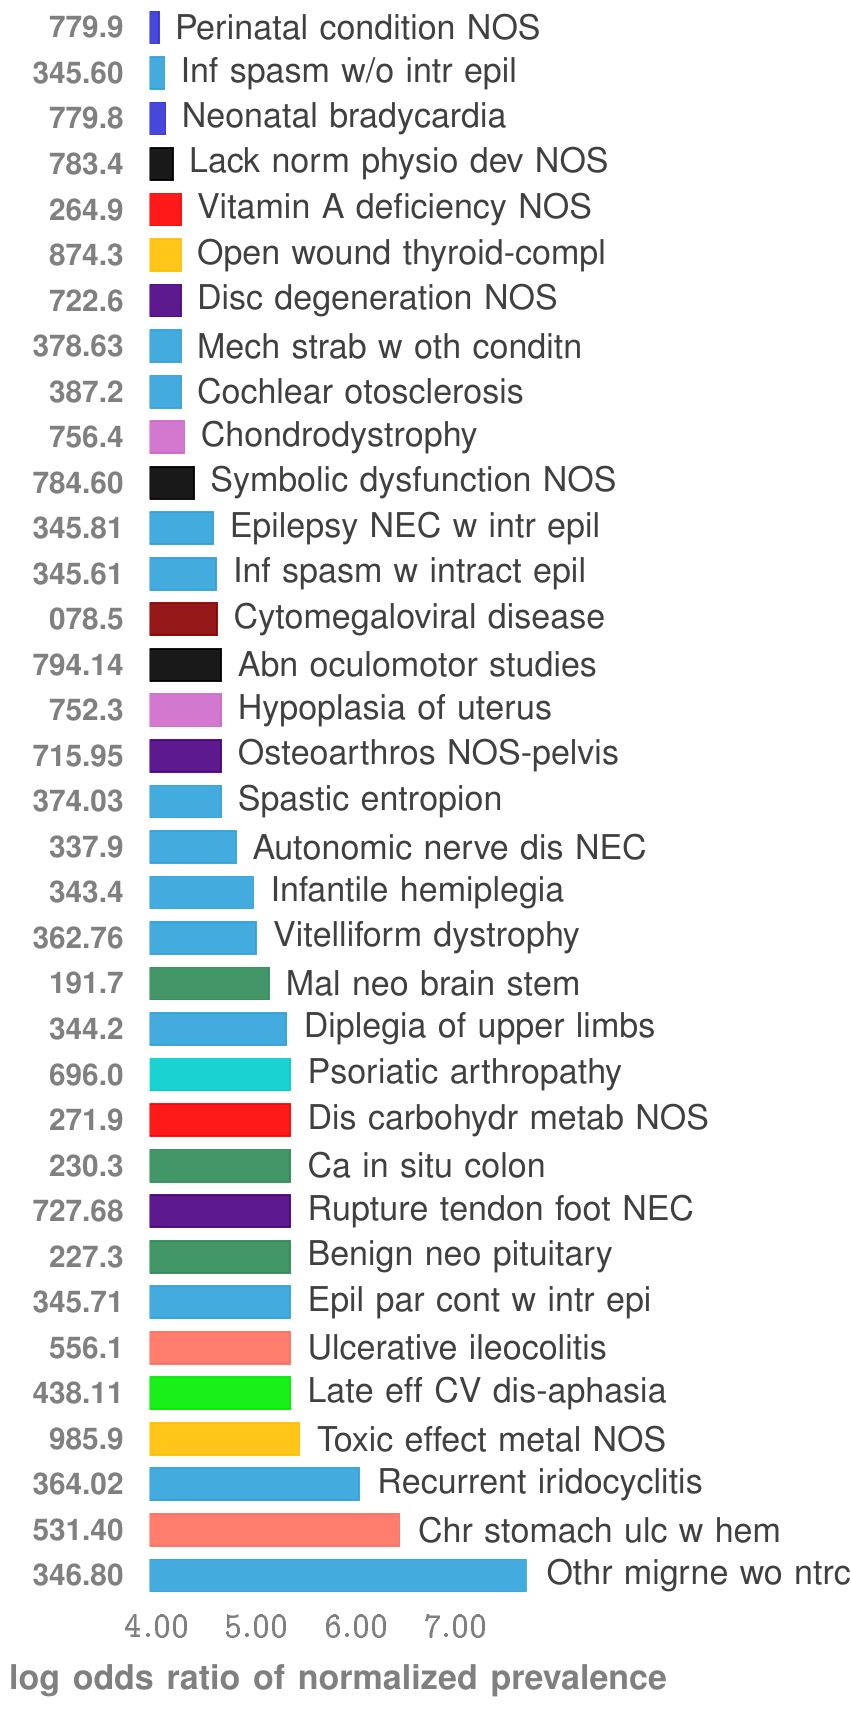
\includegraphics[height=6in,angle=90]{Figures/bars1}};
%     \node[anchor=west] (B) at (A.east) {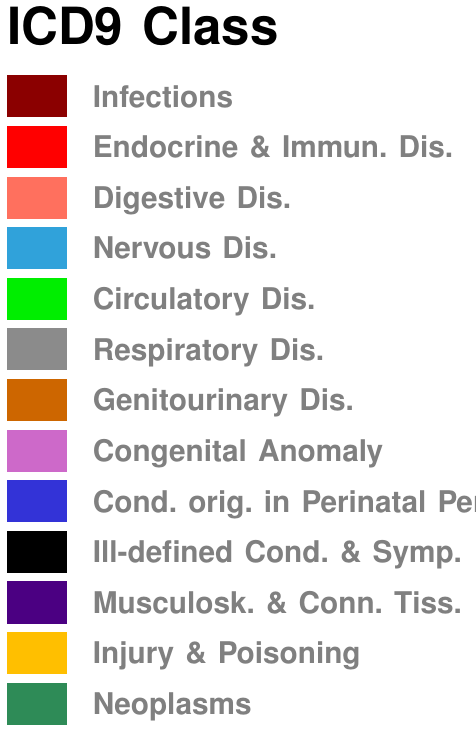
\includegraphics[height=2in,angle=0]{Figures/bars2}};
%   \end{tikzpicture}
%   \vspace{-10pt}
  
%   \captionN{Difference in occurrence frequencies of diagnostic codes between true positive (TP) and true negative (TN) predictions in males. The color coding shows the disease categories of the co-morbidities.}\label{fig3}
% \end{figure*}
% % ###########################################################
% The predictive ability of our pipeline arises from the difference in patterns of co-morbid disorders between the \treatment and the control cohorts: the diagnostic history of individual patients is not random and hides key signatures to future neuropsychiatric outcomes. %As an illustrative example, a single random patient from the Truven database is illustrated in Fig.~\ref{fig2}D.
% %Color-coding the diagnoses according to the broad ICD9 disease categories reveals that for this specific individual, infections and immunological disorders are experienced early to a much higher degree compared to other diseases, and diseases of the nervous system and sensory organs, as well as ill-defined symptoms dominate the latter period. This suggests the necessity of a deeper interrogation of the structure of co-morbid patterns, which we carried out in our preliminary investigations, as described next.
% %
% While the ASD co-morbidity burden  is reported to be high for nearly the entire spectrum of  physiological disorders, in our preliminary we find novel association patterns in normalized prevalence | the odds of experiencing a specific disorder, particularly in the early years (age~$<3$ years), normalized over all unique disorders experienced in the specified time-frame. Additionally, we only focus on  the true positives in the \treatment cohort and the true negatives in the control cohort. This  allows us to investigate  patterns that correctly disambiguate future ASD status, $i.e.$, strongly favor one outcome over the other at the individual level (as opposed to population-level prevalence rates), as shown in  Fig.~\ref{fig3} for males.

% %Additionally, we found in our preliminary studies indications of : 1) \textit{negative associations:} there are diseases that are negatively associated with ASD diagnosis with respect to normalized prevalence, $i.e.$, having those codes over-represented relative to other codes in one's diagnostic history favors ending up in the control cohort, 2) \textit{gendered impact:} there are gender-specific differences in the impact of specific disorders which will be further investigated in this study.
% %
% % \subsection*{Effect of Change In Diagnostic Criteria: Inclusion of PDD \&  Asperger's Syndrome}
% % %
% % The DSM-5 established a single category of ASD to replace
% % the subtypes of autistic disorder,
% % Asperger syndrome, and pervasive
% % developmental disorder not
% % otherwise specified in the Diagnostic
% % and Statistical Manual of Mental
% % Disorders, Fourth Edition, Text
% % Revision (DSM-IV-TR)~\cite{hyman2020identification}. This aligns with our use of diagnostic codes from ICD9 299.X as specification of an ASD diagnosis, and use GEMS mapping to 299.X from ICD10 codes when we encounter them.
% % Importantly, we found that it is  difficult to design a high performing pipeline that recognizes these ASD sub-types separately, even if we so wanted.
% %
% \subsection*{Disambiguation From Unrelated Psychiatric Phenotypes}
% %
% In our retrospective analyses,  we can discriminate between ASD and other unrelated psychiatric phenotypes. Does our pipeline pick up on any psychiatric conditions, or is it specific to ASD? We  evaluated this question, by restricting the  control  cohort in validation to  patients with at least one psychiatric code other than ASD. We get very high discrimination reaching AUCs over $90\%$ at $100-125$ weeks of age, which establishes that our pipeline is indeed largely specific to ASD.
% %
% \subsection*{Sanity Checks: Uncertainty in EHR Records}
% Recent changes in diagnostic practice, $e.g.$ increased diagnoses from individual clinicians versus prior eras that only allowed diagnosis from the gold-standard multi-disciplinary teams can  increase observed   prevalence, and  raises the possibility that  some diagnostic codes pertaining to ASD in medical history databases could be arising from less restrictive workflows, and  are susceptible to increased uncertainty.  In our study, we verified that restricting the \treatment cohort to children with at least two  distinct ASD diagnostic codes in their medical histories instead of one, has little impact on  out-of-sample predictive performance.
 
% We also found that the density of diagnostic codes in a child's medical history by itself is somewhat predictive of a future ASD diagnosis, but not at clinically significant levels.


% % \subsection*{Data Management} Data collection forms for demographic and clinical history data, database design and data
% % management procedures will be designed, created and conducted at the University of Chicago under the
% % direction of Dr. Smith. Demographic and clinical history data will be collected and entered into an HIPAA compliant secure database. Data will be entered within one day of collection and will pass
% % through rigorous quality control checks for accuracy and completeness before and after data entry.  Monthly reports will be generated  to monitor data timeliness, completeness, and
% % accuracy as well as subject flow through the study. Data sets stripped of patient identifiers will be sent
% % electronically to Dr. Chattopadhyay as needed for analysis.

%\clearpage

\bibliographystyle{naturemag}
\bibliography{aut,BibLib1}

\end{document}


% LocalWords:  neurobiological morbidities
 